%!TeX root=../document.tex

\chapter{Equations of Motion}

\section{Introduction}

\subsection{Single Element Equation}

Consider a single, unconstrained finite element with index~$k$ and~$n$ degrees of freedom.
Its configuration at time~$t$ will be described by the displacement vector~$\boldsymbol{u}_{k}(t) \in \mathbb{R}^n$ containing all the coordinates of the element's nodes.
For the kinds of elements that we will use, the equation of motion takes the form

\begin{equation}
\boldsymbol{M}_{k}\,\ddot{\boldsymbol{u}}_{k}(t) + \boldsymbol{D}_{k}\,\dot{\boldsymbol{u}}_{k}(t) + \boldsymbol{Q}_{k}(\boldsymbol{u}_{k}(t)) = \boldsymbol{P}_{k}(t).\label{eq:local-equation-of-motion}
\end{equation}

This is a nonlinear ordinary differential equation of second order for the displacements~$\boldsymbol{u}_{k}(t)$.
The matrix ~$\boldsymbol{M}_{k} \in \mathbb{R}^{n \times n}$ is called the element's mass matrix.
It defines the element's inertial forces and is constant and positive definite.
The matrix~$\boldsymbol{D}_{k} \in \mathbb{R}^{n \times n}$ is the element's damping matrix and defines a linear relationship between the velocities~$\dot{\boldsymbol{u}}_{k}(t)$ and the resulting damping forces.
It is also constant and positive semi-definite.
The only nonlinear term in the equation is the vector of elastic forces,~$\boldsymbol{Q}_{k} \in \mathbb{R}^n$, which depends on the displacements in an arbitrary way.

In the following chapters we are going to derive the components of this element equation for the various elements used in VirtualBow, but first let's consider the overall system that results from combining multiple such elements.

\newpage
\subsection{Overall System Equation}

If the overall finite element system has a total of~$N$ degrees of freedom, it's configuration can be described by the global displacement vector~$\boldsymbol{u}(t) \in \mathbb{R}^{N}$.
The local element displacements~$\boldsymbol{u}_{k}$ are now no longer independent but instead directly related to the global displacements of the system they are part of.
In our case these connectivity constraints can be written as

\begin{equation}
\boldsymbol{u}_{k}(t) = \boldsymbol{A}_{k}\,\boldsymbol{u}(t) + \boldsymbol{b}_{k},\label{eq:kinematics-local-global}
\end{equation}

where~$\boldsymbol{A}_{k} \in \mathbb{R}^{\mathlarger{n} \times N}$ describes a linear transformation and~$\boldsymbol{b}_{k} \in \mathbb{R}^{N}$ describes a constant translation or offset for the respective element displacements.
Applying this kinematic relationship to the local equations of motion~(\ref{eq:local-equation-of-motion}) leads to the element equations expressed in the global coordinates~$\boldsymbol{u}(t)$,

\begin{equation}
\boldsymbol{A}_{k}^\intercal\boldsymbol{M}_{k}\boldsymbol{A}_{k}\,\ddot{\boldsymbol{u}}(t) + \boldsymbol{A}_{k}^\intercal\boldsymbol{D}_{k}\,\boldsymbol{A}_{k}\,\dot{\boldsymbol{u}}(t) + \boldsymbol{A}_{k}^\intercal\boldsymbol{Q}_{k}(\boldsymbol{A}_{k}\,\boldsymbol{u}(t) + \boldsymbol{b}_{k}) = \boldsymbol{A}_{k}^\intercal\boldsymbol{P}_{k}.
\end{equation}

And finally, by summing up the element contributions, the equation of motion of the overall system turns out to have the same structure as the element equations,

\begin{equation}
\boldsymbol{M}\,\ddot{\boldsymbol{u}} + \boldsymbol{D}\,\dot{\boldsymbol{u}} + \boldsymbol{Q}(\boldsymbol{u}) = \boldsymbol{P}(t)\label{eq:global-equation-of-motion}
\end{equation}

where the global mass matrix $\boldsymbol{M} \in \mathbb{R}^{N \times N}$, damping matrix $\boldsymbol{D} \in \mathbb{R}^{N \times N}$, internal forces~$\boldsymbol{Q} \in \mathbb{R}^{N}$ and external forces $\boldsymbol{P} \in \mathbb{R}^{N}$ are calculated from the local element matrices as

\begin{align}
\boldsymbol{M} &= \sum_{k} \boldsymbol{A}_{k}^\intercal\boldsymbol{M}_{k}\boldsymbol{A}_{k} \\
\boldsymbol{D} &= \sum_{k} \boldsymbol{A}_{k}^\intercal\boldsymbol{D}_{k}\boldsymbol{A}_{k} \\
\boldsymbol{Q} &= \sum_{k} \boldsymbol{A}_{k}^\intercal\boldsymbol{Q}_{k}(\boldsymbol{A}_{k}\,\boldsymbol{u} + \boldsymbol{b}_{k}) \\
\boldsymbol{P} &= \sum_{k} \boldsymbol{A}_{k}^\intercal\boldsymbol{P}_{k}
\end{align}

In order to solve the equations of motion for equilibrium we're later going to need the derivative of the elastic forces with respect to the displacements, which is called the tangent stiffness matrix~$\boldsymbol{K} \in \mathbb{R}^{N \times N}$ of the system and can be calculated from the element's local tangent stiffness matrices~$\boldsymbol{K}_{k} = \partial \boldsymbol{Q}_{k} / \partial \boldsymbol{u}_{k}$ as

\begin{align}
\boldsymbol{K}(\boldsymbol{u}) &= \frac{\partial \boldsymbol{Q}}{\partial \boldsymbol{u}} = \frac{\partial}{\partial \boldsymbol{u}} \sum_{k} \boldsymbol{A}_{k}^\intercal\boldsymbol{Q}_{k}(\boldsymbol{A}_{k}\,\boldsymbol{u} + \boldsymbol{b}_{k}) \notag \\
&= \sum_{k} \boldsymbol{A}_{k}^\intercal \frac{\partial}{\partial \boldsymbol{u}_{k}}\boldsymbol{Q}_{k}(\boldsymbol{A}_{k}\,\boldsymbol{u} + \boldsymbol{b}_{k})\,\frac{\partial \boldsymbol{u}_{k}}{\partial \boldsymbol{u}} = \sum_{k} \boldsymbol{A}_{k}^\intercal \boldsymbol{K}_{k} \boldsymbol{A}_{k}.
\end{align}

\subsection{Connectivity Constraints}

The transformation matrices $\boldsymbol{A}$ and $\boldsymbol{b}$ are not arbitrary.
Any element displacement $u_{i}$, where $i$ is now the index in the local vector, only depends on the corresponding global displacement $\overline{u}_{m(i)}$, where $m(i)$ is a mapping from local to global index.
The required relationship between the two is

$$u_{i} = a_{i}\,\overline{u}_{m(i)} + b_{i}$$

If $a_{i}$ is zero, the corresponding element displacement is fixed to $b_{i}$.
In order to understand how this simplifies the calculation of the transformations, consider two displacements $u_{i}$ and $u_{j}$,

\begin{align*}
u_{i} &= a_{i}\,\overline{u}_{m(i)} + b_{i} \\
u_{j} &= a_{j}\,\overline{u}_{m(j)} + b_{j}
\end{align*}

The transformation with respect to those two displacements takes the following form, where each row in $\boldsymbol{A}$ only contains one non-zero element $a$ that relates two displacements:

$$
\underbrace{
\begin{bmatrix}
\vdots \\ u_{i} \\ \vdots \\ u_{j} \\ \vdots
\end{bmatrix}
}_{\boldsymbol{u}_{k}}
=
\underbrace{
\begin{bmatrix}
& \vdots & \vdots & \\
0 \hdots 0 & a_{i} & 0 & 0 \hdots 0 \\
& \vdots & \vdots & \\
0 \hdots 0 & 0 & a_{j} & 0 \hdots 0 \\
& \vdots & \vdots &
\end{bmatrix}
}_{\boldsymbol{A}_{k}}
\underbrace{
\begin{bmatrix}
\vdots \\ u_{m(i)} \\ \vdots \\ u_{m(j)} \\ \vdots
\end{bmatrix}
}_{\boldsymbol{u}}
+
\underbrace{
\begin{bmatrix}
\vdots \\ b_{i} \\ \vdots \\ b_{j} \\ \vdots
\end{bmatrix}
}_{\boldsymbol{b}_{k}}
$$

By transposing this matrix, we can write the dependence of the global internal forces $\boldsymbol{Q}$ on the local internal forces $\boldsymbol{Q}_{k}$ as:

$$
\underbrace{
\begin{bmatrix}
\vdots \\ \overline{Q}_{m(i)} \\ \vdots \\ \overline{Q}_{m(j)} \\ \vdots
\end{bmatrix}
}_{\boldsymbol{Q}}
=
\underbrace{
\begin{bmatrix}
& 0 & & 0 & \\
& \vdots & & \vdots & \\
\hdots & a_{i} & \hdots & 0 & \hdots \\
\hdots & 0 & \hdots & a_{j} & \hdots \\
& \vdots & & \vdots & \\
& 0 & & 0 &
\end{bmatrix}
}_{\boldsymbol{A}^\intercal}
\underbrace{
\begin{bmatrix}
\vdots \\ Q_{i} \\ \vdots \\ Q_{j} \\ \vdots
\end{bmatrix}
}_{\boldsymbol{Q}_{k}}
$$

Which can be written as the scalar relationship $\overline{Q}_{m(i)} = a_{i}\,Q_{i}$.
Similarly, the dependence of the global mass matrix $\boldsymbol{M}$ on the local mass matrix $\boldsymbol{M}_{k}$ is

$$
\underbrace{
\begin{bmatrix}
& \vdots & \\
\hdots & \overline{M}_{m(i),m(j)} & \hdots \\
& \vdots &
\end{bmatrix}
}_{\boldsymbol{M}}
=
\underbrace{
\begin{bmatrix}
& 0 & & 0 & \\
& \vdots & & \vdots & \\
\hdots & a_{i} & \hdots & 0 & \hdots \\
\hdots & 0 & \hdots & a_{j} & \hdots \\
& \vdots & & \vdots & \\
& 0 & & 0 &
\end{bmatrix}
}_{\boldsymbol{A}_{k}^\intercal}
\underbrace{
\begin{bmatrix}
& \vdots & \\
\hdots & M_{i,j} & \hdots \\
& \vdots &
\end{bmatrix}
}_{\boldsymbol{M}_{k}}
\underbrace{
\begin{bmatrix}
& \vdots & \vdots & \\
0 \hdots 0 & a_{i} & 0 & 0 \hdots 0 \\
& \vdots & \vdots & \\
0 \hdots 0 & 0 & a_{j} & 0 \hdots 0 \\
& \vdots & \vdots &
\end{bmatrix}
}_{\boldsymbol{A}_{k}}
$$

Which can be written as $\overline{M}_{m(i),m(j)} = a_{i}\,a_{j}\,M_{i,j}$.
Analogous for the transformation of $\boldsymbol{P}$, $\boldsymbol{D}$ and $\boldsymbol{K}$.
These results show that it is actually not necessary to perform any matrix operations with $\boldsymbol{A}$, we don't even need to construct it at all.
Instead, the scalar relationships can be used to transform the element matrices and add them to the respective global matrices in one go.

% Quick python script for verification
%
% import numpy as np
%
% n = 6
% N = 10
%
% i = 2
% j = 4
%
% ki = 5
% kj = 8
%
% ai = 3
% aj = 7
%
% Mij = 11
% Qi = 13
%
% M_local = np.zeros([n, n])
% M_local[i, j] = Mij
%
% Q_local = np.zeros([n])
% Q_local[i] = Qi
%
% A = np.zeros([n, N])
% A[i, ki] = ai
% A[j, kj] = aj
%
% M_global = A.T @ M_local @ A
% Q_global = A.T @ Q_local
%
% print(M_local)
% print(M_global)
% print(Q_local)
% print(Q_global)

\newpage
\section{Mass Element}

The point mass is the most simple element.
Figure~\ref{fig:elements:point-mass} shows its definition: A mass~$m$ is placed in a cartesian coordinate system. Its position is described by the displacements~$u_0(t)$ and~$u_1(t)$ along the coordinate axes.
The external forces~$p_0(t)$ and~$p_1(t)$ are acting in the direction of the respective displacements.

\begin{figure}[h]
\centering
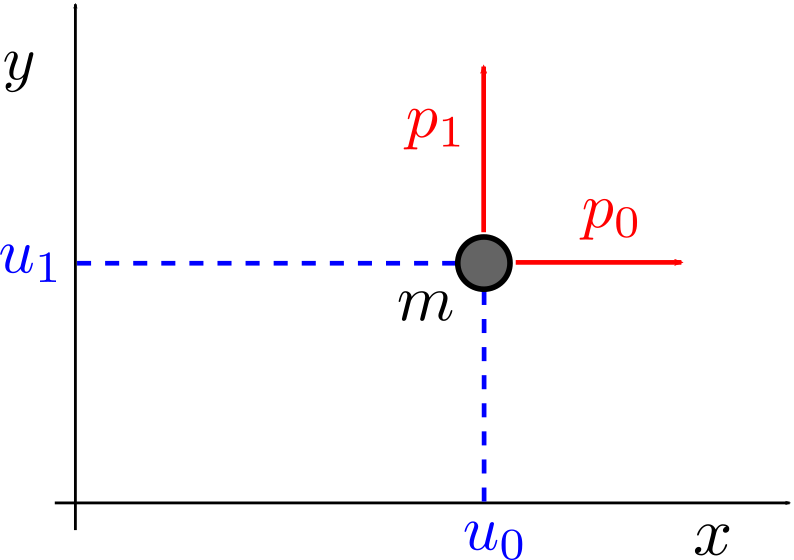
\includegraphics[width=0.4\textwidth]{figures/elements/mass-element}
\caption{Point mass element}
\label{fig:elements:point-mass}
\end{figure}

The equation of motion for this system can be written down directly by using Newton's second law of motion:

\begin{equation}
\underbrace{
\begin{bmatrix}
m & 0\\
0 & m
\end{bmatrix}
}_{\boldsymbol{M}}
\underbrace{
\begin{bmatrix}
\ddot{u}_0\\
\ddot{u}_1
\end{bmatrix}
}_{\boldsymbol{\ddot{u}}}
+
\underbrace{
\begin{bmatrix}
0\\
0
\end{bmatrix}
}_{\boldsymbol{q}(\boldsymbol{u},\,\dot{\boldsymbol{u}})}
=
\underbrace{
\begin{bmatrix}
p_0\\
p_1
\end{bmatrix}
}_{\boldsymbol{p}(t)}
\end{equation}

This immediately gives us the element's mass matrix, internal forces (which are zero) and external forces.
Because the internal forces are zero, the tangent stiffness and damping matrices are zero as well:

\begin{equation}
\boldsymbol{K} = \frac{\partial \boldsymbol{q}}{\partial \boldsymbol{u}} =
\begin{bmatrix}
0 & 0\\
0 & 0
\end{bmatrix},
\quad
\boldsymbol{D} = \frac{\partial \boldsymbol{q}}{\partial \dot{\boldsymbol{u}}} =
\begin{bmatrix}
0 & 0\\
0 & 0
\end{bmatrix}
\end{equation}

\newpage
\section{Bar Element}

A bar only transfers forces in longitudinal direction, it has no bending stiffness. Figure~\ref{fig:bar-element-1} shows a bar with an initial length of~$l$ that is subjected to a normal force~$N$ which causes it to elongate by~$\Delta l$.

\begin{figure}[h]
\centering
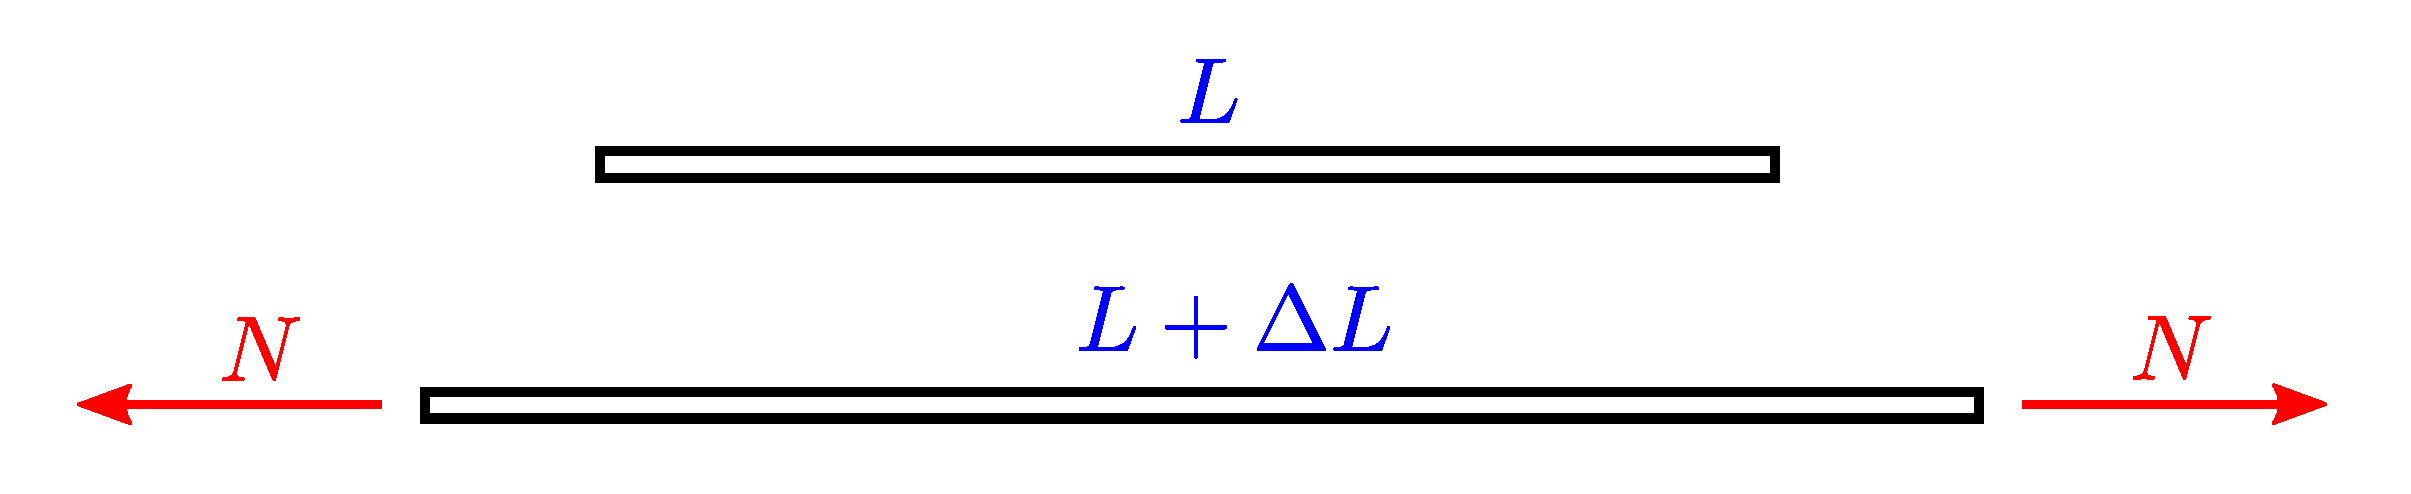
\includegraphics[width=0.75\textwidth]{figures/elements/bar-element-1}
\caption{Elongation of a bar under load}
\label{fig:bar-element-1}
\end{figure}

In order to simulate the damping properties of the string, a viscoelastic material model of the form

\begin{equation}
\sigma = E\,\varepsilon + \eta\,\dot{\varepsilon}
\end{equation}

is chosen. Here $E$ is the elastic modulus and $\eta$ the viscosity of the material. This model is called the Kelvin-Voigt model and combines linear elastic and linear viscous behaviour. The normal force in the bar given a constant cross section area $A$ is therefore

\begin{align}
N &= \sigma A \notag \\
&= EA\,\varepsilon + \eta A\,\dot{\varepsilon} \notag \\
&= \frac{EA}{l}\,\Delta l + \frac{\eta A}{l}\,\Delta \dot{l} \\
&= k\,\Delta l + d\,\Delta \dot{l}.\label{eq:bar-constitutive}
\end{align}

The product~$EA$ is also called the longitudinal stiffness.
By setting~$\varepsilon = \frac{\Delta l}{l}$ it was implicitly assumed that the strain is constant over the length of the element.
The resulting normal force (\ref{eq:bar-constitutive}) has the same form as a linear spring with stiffness~$k = \frac{EA}{l}$ and damping~$d = \frac{\eta A}{l}$.

The bar is now placed between the two nodes A and B as shown in figure~\ref{fig:bar-element-2}. Its configuration is described by the nodal displacements~$\boldsymbol{u} = (u_0,\,u_1,\,u_2,\,u_3)^\mathsf{T}$.

\begin{figure}[h]
\centering
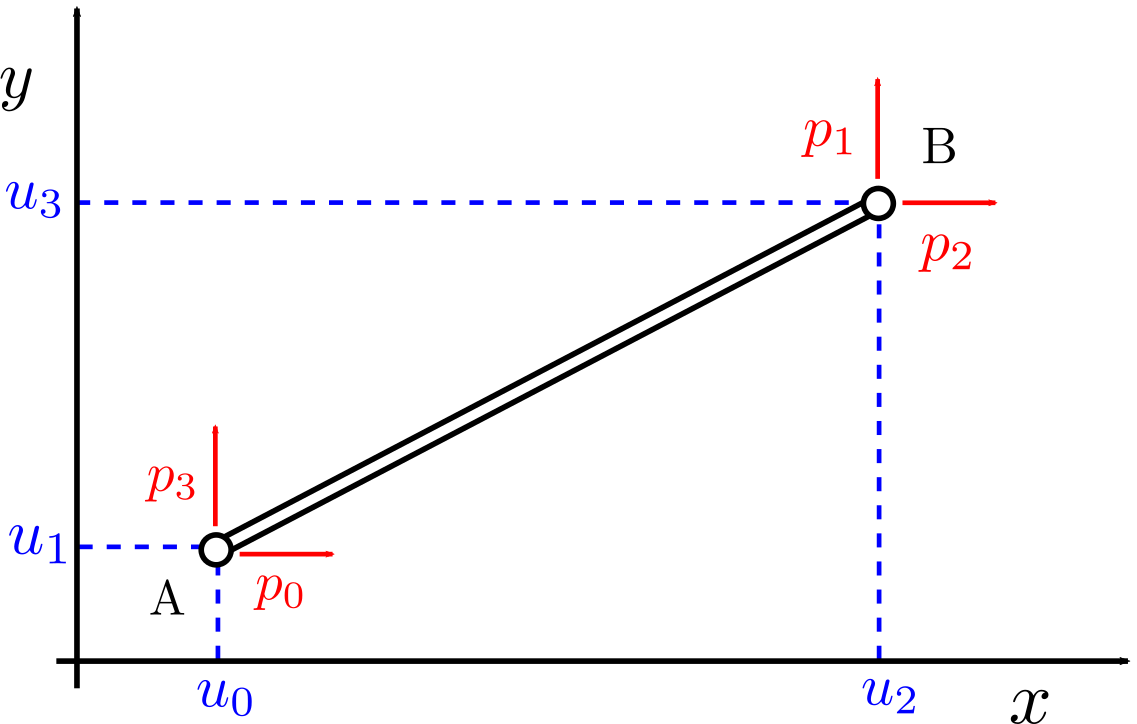
\includegraphics[width=0.6\textwidth]{figures/elements/bar-element-2}
\caption{Bar element}
\label{fig:bar-element-2}
\end{figure}

The position vectors of the two nodes are given by

\begin{equation}
\boldsymbol{r}_A =
\begin{bmatrix} u_0 \\ u_1 \end{bmatrix}, \quad
\boldsymbol{r}_B =
\begin{bmatrix} u_2 \\ u_3 \end{bmatrix}.\label{bar:node-positions}
\end{equation}

The mass of the element is assumed to be concentrated at the nodes, so that each of them is carrying half of the total mass.
This is called a lumped mass approach and will later lead to a constant, diagonal mass matrix.
For a bar with density~$\rho$ the mass of a node is therefore~$\frac{1}{2}\rho A L$. With this in mind we can write down Newton's second law of motion for each of the two nodes,
%
\begin{align}
\frac{\rho A L}{2}\,\ddot{\boldsymbol{r}}_A = \boldsymbol{q}_A + \boldsymbol{p}_A,\label{eq:bar-newton-1}\\
\frac{\rho A L}{2}\,\ddot{\boldsymbol{r}}_B = \boldsymbol{q}_B + \boldsymbol{p}_B.\label{eq:bar-newton-2}
\end{align}

Here,~$\boldsymbol{q}_A$,~$\boldsymbol{q}_B$ are the elastic forces that the bar exerts to the respective nodes and~$\boldsymbol{p}_A$,~$\boldsymbol{p}_B$ are the externally applied loads. The elastic forces can be obtained by multiplying the scalar normal force~$N$ in the bar~(\ref{eq:bar-constitutive}) with the tangent vector of the connecting line between the two nodes to account for the direction.
With defining $\Delta\boldsymbol{r} = \boldsymbol{r}_B - \boldsymbol{r}_A$ they become
%
\begin{equation}
\boldsymbol{q}_A = N\cdot\frac{\Delta\boldsymbol{r}}{\lVert\Delta\boldsymbol{r}\rVert},\quad \boldsymbol{q}_B = -\boldsymbol{q}_A.\label{eq:bar-elastic}
\end{equation}

The elongation~$\Delta l$ can be calculated by subtracting the initial length of the element from its actual length,
%
\begin{align}
\Delta L &= \lVert\Delta\boldsymbol{r}\rVert - l,\label{eq:bar-elongation} \\
\Delta \dot{L} &= \frac{d}{dt}\,\lVert\Delta\boldsymbol{r}\rVert = \frac{\Delta\boldsymbol{r}^\intercal}{\lVert\Delta\boldsymbol{r}\rVert}\Delta\dot{\boldsymbol{r}}.\label{eq:bar-elongation-velocity}
\end{align}

Combining equations~(\ref{eq:bar-newton-1}),~(\ref{eq:bar-newton-2}) with~(\ref{eq:bar-elastic}),~(\ref{eq:bar-elongation}) and (\ref{eq:bar-elongation-velocity}) leads to the element's equation of motion,

\begin{equation}
\frac{\rho Al}{2}
\begin{bmatrix}
\ddot{\boldsymbol{r}}_A \\ \ddot{\boldsymbol{r}}_B
\end{bmatrix}
+
\frac{1}{\lVert\Delta\boldsymbol{r}\rVert}
\left(
\frac{\eta A}{l}
\frac{\Delta\boldsymbol{r}^\intercal\Delta\dot{\boldsymbol{r}}}{\lVert\Delta\boldsymbol{r}\rVert}
+
\frac{EA}{L}\left(\lVert\Delta\boldsymbol{r}\rVert - l\right)
\right)
\begin{bmatrix}
-\Delta\boldsymbol{r} \\ \phantom{-}\Delta\boldsymbol{r}
\end{bmatrix}
=
\begin{bmatrix}
\boldsymbol{p}_A \\ \boldsymbol{p}_B
\end{bmatrix}.
\end{equation}

\textcolor{red}{TODO: Redo remaining calculations from here on...}

With~(\ref{bar:node-positions}) and the abbreviations $\Delta x = u_{2} - u_{0}$, $\Delta y = u_{3} - u_{1}$ this expands to

\begin{equation}
\underbrace{
\frac{\rho A L}{2}
\begin{bmatrix}
1\\
& 1\\
&& 1\\
&&& 1
\end{bmatrix}
}_{\boldsymbol{M}}
\underbrace{
\begin{bmatrix}
\ddot{u}_0\\
\ddot{u}_1\\
\ddot{u}_2\\
\ddot{u}_3
\end{bmatrix}
}_{\boldsymbol{\ddot{u}}}
+
\underbrace{
\frac{\eta A}{L}
\begin{bmatrix}
-\Delta \dot{x}\\
-\Delta \dot{y}\\
\ \ \Delta \dot{x}\\
\ \ \Delta \dot{y}
\end{bmatrix}
+
\frac{EA}{L}\left(1 - \frac{L}{\sqrt{\Delta x^2 + \Delta y^2}}\right)
\begin{bmatrix}
-\Delta x\\
-\Delta y\\
\ \ \Delta x\\
\ \ \Delta y
\end{bmatrix}
}_{\boldsymbol{q}(\boldsymbol{u},\,\dot{\boldsymbol{u}})}
=
\underbrace{
\begin{bmatrix}
p_0\\
p_1\\
p_2\\
p_3
\end{bmatrix}
}_{\boldsymbol{p}}.
\end{equation}

Note that the vector~$\boldsymbol{q}$ of internal forces depends on the displacements in a nonlinear way despite the bar itself being considered linear-elastic. The nonlinearity arises only from the geometry of the arbitrarily large nodal displacements. This is called geometric nonlinearity as opposed to material nonlinearity.

Deriving the internal forces with respect to $\boldsymbol{u}$ results in the tangent stiffness matrix
%
\begin{align*}
\boldsymbol{K} = \frac{\partial \boldsymbol{q}}{\partial \boldsymbol{u}} &=
\frac{EA}{L}\left(1 - \frac{L}{\sqrt{\Delta x^2 + \Delta y^2}}\right)
\begin{bmatrix}
1 & 0 & -1 & 0\\
0 & 1 & 0 & -1\\
-1 & 0 & 1 & 0\\
0 & -1 & 0 & 1
\end{bmatrix}\\
&+
\frac{EA}{(\sqrt{\Delta x^2 + \Delta y^2})^{3}}
\begin{bmatrix}
\Delta x^2 & \Delta x \Delta y & -\Delta x^2 & -\Delta x \Delta y\\
\Delta x \Delta y & \Delta y^2 & -\Delta x \Delta y & - \Delta y^2\\
-\Delta x^2 & -\Delta x \Delta y & \Delta x^2 & \Delta x \Delta y\\
-\Delta x \Delta y & -\Delta y^2 & \Delta x \Delta y & \Delta y^2
\end{bmatrix}.\\
\end{align*}

Similarly, deriving the internal forces with respect to $\dot{\boldsymbol{u}}$ results in the tangent damping matrix
%
\begin{align*}
\boldsymbol{D} = \frac{\partial \boldsymbol{q}}{\partial \dot{\boldsymbol{u}}} &=
\frac{\eta A}{L}
\begin{bmatrix}
1 & 0 & -1 & 0\\
0 & 1 & 0 & -1\\
-1 & 0 & 1 & 0\\
0 & -1 & 0 & 1
\end{bmatrix}.
\end{align*}

\newpage
\section{Bar Element (Systematic)}

Define the length $s \in [0,\,l_{0}]$ along the undeformed bar and the position vector $\boldsymbol{r}(s) = [x(s),\,y(s)]^\intercal$ of each point in the bar.
As coordinates, we chose the vector $\boldsymbol{u}(t) = [\boldsymbol{r}_{0}(t),\,\boldsymbol{r}_{1}(t)]^\intercal = [x_0,\,y_0,\,x_1,\,y_1]^\intercal$

Then approximate the continuous position field by linear interpolation,

\begin{align}
\boldsymbol{r}(s,\,\boldsymbol{u}) &= \left(1 - \frac{s}{l_{0}}\right)\,\boldsymbol{r}_{0} + \frac{s}{l_{0}}\,\boldsymbol{r}_{1} =
\underbrace{
\begin{bmatrix}
1 - \nicefrac{s}{l_{0}} & 0  & \nicefrac{s}{l_{0}} & 0 \\
0 & 1 - \nicefrac{s}{l_{0}} & 0 & \nicefrac{s}{l_{0}}
\end{bmatrix}
}_{\boldsymbol{S}(s)}
\underbrace{
\begin{bmatrix}
\boldsymbol{r}_{0} \\
\boldsymbol{r}_{1}
\end{bmatrix}
}_{\boldsymbol{u}(t)}
\end{align}

Which is expressed as a product of the time-independent shape function matrix $\boldsymbol{S}(s)$ and the time-dependent nodal displacements $\boldsymbol{u}(t)$.

The mass matrix is derived from the kinetic energy of the element,

\begin{align}
T &= \frac{1}{2}\int_{0}^{l_{0}} \rho A\,\dot{\boldsymbol{r}}^\intercal\dot{\boldsymbol{r}}\,ds \\
&= \frac{1}{2} \dot{\boldsymbol{u}}^\intercal \underbrace{\left( \rho A \int_{0}^{l} \boldsymbol{S}^\intercal \boldsymbol{S}\,ds \right)}_{\boldsymbol{M}} \dot{\boldsymbol{u}}
\end{align}

Evaluating the integral leads to the constant mass matrix

\begin{equation}
\boldsymbol{M} = \rho Al_{0} \begin{bmatrix}
\nicefrac{1}{3} & 0 & \nicefrac{1}{6} & 0\\
0 & \nicefrac{1}{3} & 0 & \nicefrac{1}{6}\\
\nicefrac{1}{6} & 0 & \nicefrac{1}{3} & 0\\
0 & \nicefrac{1}{6} & 0 & \nicefrac{1}{3}
\end{bmatrix}.
\end{equation}

Longitudinal strain and strain rate:

\begin{align}
\varepsilon &= \lVert\boldsymbol{r}'\rVert - 1 = \lVert \boldsymbol{S}'\boldsymbol{u} \rVert - 1 \\
\dot{\varepsilon} &= \left(\frac{\partial \varepsilon}{\partial \boldsymbol{r}'}\right)^\intercal\frac{\partial \boldsymbol{r}'}{\partial t} = \frac{\boldsymbol{r}'^\intercal\dot{\boldsymbol{r}'}}{\lVert\boldsymbol{r}'\rVert} = \frac{\boldsymbol{u}^\intercal\boldsymbol{S}'^\intercal\boldsymbol{S}' \dot{\boldsymbol{u}}}{\lVert \boldsymbol{S}'\boldsymbol{u} \rVert}
\end{align}

Both are actually constant over the length of the element due to the choice of linear interpolation functions, which can be shown by evaluating the first derivative of the shape function matrix,

\begin{align}
\boldsymbol{S}' &= \frac{1}{l_{0}}
\begin{bmatrix}
\phantom{-}\boldsymbol{I}_{2 \times 2} & -\boldsymbol{I}_{2 \times 2}
\end{bmatrix} \\
\boldsymbol{S}'^\intercal\boldsymbol{S}' &= \frac{1}{l_{0}^2}
\begin{bmatrix}
\phantom{-}\boldsymbol{I}_{2 \times 2} & -\boldsymbol{I}_{2 \times 2} \\
-\boldsymbol{I}_{2 \times 2} & \phantom{-}\boldsymbol{I}_{2 \times 2}
\end{bmatrix}
\end{align}

%We can evaluate $\boldsymbol{r}'$ and $\lVert\boldsymbol{r}'\rVert$ in terms of the nodal positions as:

%\begin{align}
%\boldsymbol{r}' &= \boldsymbol{S}'\boldsymbol{u} = \frac{1}{l_{0}}\left(\boldsymbol{r}_{1} - \boldsymbol{r}_{0}\right) = \frac{\Delta\boldsymbol{r}}{l_{0}} \\
%\lVert\boldsymbol{r}'\rVert &= \frac{\lVert\Delta\boldsymbol{r}\rVert}{l_{0}} = \frac{l}{l_{0}}
%\end{align}

%With those, the strain can be written as

%\begin{equation}
%\varepsilon = \frac{l}{l_{0}} - 1, \quad \dot{\varepsilon} = \frac{\Delta\boldsymbol{r}^\intercal\Delta\dot{\boldsymbol{r}}}{l\,l_{0}}
%\end{equation}

%Here we used the current length $l = \lVert\Delta\boldsymbol{r}\rVert$ of the bar.

Material law (Kelvin-Voigt material):

\begin{align}
\sigma &= E\,\varepsilon + \eta\,\dot{\varepsilon} \\
N &= \sigma A = EA\,\varepsilon + \eta A\,\dot{\varepsilon}
\end{align}

Virtual work of the internal forces:

\begin{align}
\delta W_{I} &= \int_{V} \sigma\,\delta\varepsilon\,dV = \int_{0}^{l_{0}} N\,\delta\varepsilon\,ds = \int_{0}^{l_{0}} \left( EA\,\varepsilon + \eta A\,\dot{\varepsilon} \right)\,\delta\varepsilon\,ds \\
&= \int_{0}^{l_{0}} \left( EA\,\varepsilon + \eta A\,\dot{\varepsilon} \right)\,\frac{\partial \varepsilon}{\partial \boldsymbol{u}}\delta\boldsymbol{u}\,ds
\end{align}

Therefore the internal forces are

\begin{align}
\boldsymbol{Q} &= \int_{0}^{l_{0}} \left( EA\,\varepsilon + \eta A\,\dot{\varepsilon} \right)\,\frac{\partial \varepsilon}{\partial \boldsymbol{u}}\,ds \\
&= \left( EA\,\varepsilon + \eta A\,\dot{\varepsilon} \right)\,l_{0}\frac{\partial \varepsilon}{\partial \boldsymbol{u}} \\
&= Nl_{0}\frac{\partial \varepsilon}{\partial \boldsymbol{u}}
\end{align}

The following partial derivatives of the strain with respect to the nodal coordinates will be required later:

\begin{align}
\frac{\partial \varepsilon}{\partial \boldsymbol{u}} &= \left(\frac{\partial \varepsilon}{\partial \boldsymbol{r}'}\right)^\intercal\frac{\partial \boldsymbol{r}'}{\partial \boldsymbol{u}} = \frac{\boldsymbol{r}'^\intercal\boldsymbol{S}'}{\lVert \boldsymbol{r}' \rVert} = \frac{\boldsymbol{u}^\intercal\boldsymbol{S}'^\intercal\boldsymbol{S}'}{\lVert \boldsymbol{r}' \rVert} = \frac{\boldsymbol{S}'^\intercal\boldsymbol{S}'\boldsymbol{u}}{\lVert \boldsymbol{S}'\boldsymbol{u} \rVert} \\
\frac{\partial^2 \varepsilon}{\partial \boldsymbol{u}^2} &= \boldsymbol{S}'^\intercal\left(\frac{1}{\lVert\boldsymbol{r}'\rVert}\left(\boldsymbol{I}_{2 \times 2} - \frac{\boldsymbol{r}'\boldsymbol{r}'^\intercal}{\lVert\boldsymbol{r}'\rVert^2}\right) \right)\boldsymbol{S}' \\
\frac{\partial \dot{\varepsilon}}{\partial \boldsymbol{u}} &= \frac{\partial}{\partial t}\frac{\partial \varepsilon}{\partial \boldsymbol{u}} = \frac{\partial}{\partial \boldsymbol{u}}\left( \frac{\partial \varepsilon}{\partial \boldsymbol{u}} \right)\frac{\partial\boldsymbol{u}}{\partial t} = \frac{\partial^2 \varepsilon}{\partial \boldsymbol{u}^2}\dot{\boldsymbol{u}} \\
\frac{\partial \dot{\varepsilon}}{\partial \dot{\boldsymbol{u}}} &= \frac{\boldsymbol{S}'^\intercal\boldsymbol{S}'\boldsymbol{u}}{\lVert \boldsymbol{S}'\boldsymbol{u} \rVert} \\
\end{align}

Derivatives of the normal force:

\begin{align}
\frac{\partial N}{\partial \boldsymbol{u}} &= EA\frac{\partial \varepsilon}{\partial \boldsymbol{u}} + \eta A\frac{\partial \dot{\varepsilon}}{\partial \boldsymbol{u}} \\
\frac{\partial N}{\partial \dot{\boldsymbol{u}}} &= \eta A\frac{\partial \dot{\varepsilon}}{\partial \dot{\boldsymbol{u}}}
\end{align}


Tangent stiffness and damping matrices:

\begin{align}
\boldsymbol{K} &= \frac{\partial \boldsymbol{Q}}{\partial \boldsymbol{u}} = l_{0}\frac{\partial N}{\partial \boldsymbol{u}}\frac{\partial \varepsilon}{\partial \boldsymbol{u}} + Nl_{0}\frac{\partial^2 \varepsilon}{\partial \boldsymbol{u}^2} \\
\boldsymbol{D} &= \frac{\partial \boldsymbol{Q}}{\partial \dot{\boldsymbol{u}}} = l_{0}\frac{\partial N}{\partial \dot{\boldsymbol{u}}}\frac{\partial \varepsilon}{\partial \boldsymbol{u}}
\end{align}



\newpage

%\begin{align}
%\frac{\partial \varepsilon}{\partial \boldsymbol{u}} &= \frac{\partial \varepsilon}{\partial \boldsymbol{r}'}\frac{\partial \boldsymbol{r}'}{\boldsymbol{u}} = \frac{ \boldsymbol{r}'^\intercal\boldsymbol{S}'}{\lVert \boldsymbol{r}' \rVert} = \frac{\frac{1}{l_{0}}\Delta\boldsymbol{r}\frac{1}{l_{0}}\begin{bmatrix}
%-\boldsymbol{I},\,\boldsymbol{I}
%\end{bmatrix}}{\frac{1}{l_{0}}\lVert\Delta\boldsymbol{r}\rVert} \\
%&= \frac{1}{l\,l_{0}}
%\begin{bmatrix}
%-\Delta\boldsymbol{r} \\
%\Delta\boldsymbol{r}
%\end{bmatrix}
%\end{align}

%Putting everything together and introducing the stiffness $k = EA/l_{0}$ and damping $d = \eta A/l_{0}$:

%\begin{align}
%N &= \frac{EA}{l_{0}}\left(l - l_{0}\right) + \frac{\eta A}{l_{0}}\frac{\Delta\boldsymbol{r}^\intercal\Delta\dot{\boldsymbol{r}}}{l} \\
%\boldsymbol{Q} &= \frac{N}{l}
%\begin{bmatrix}
%-\Delta\boldsymbol{r} \\
%\phantom{-}\Delta\boldsymbol{r}
%\end{bmatrix}
%\end{align}

%In order to determine the tangent stiffness and damping matrices we first compute the partial derivatives of the normal force $N$,

%\begin{align}
%\frac{\partial N}{\partial \boldsymbol{u}} &= \frac{\partial}{\partial \Delta\boldsymbol{r}}\left( \frac{EA}{l_{0}}\left(\lVert\Delta\boldsymbol{r}\rVert - l_{0}\right) + \frac{\eta A}{l_{0}}\frac{\Delta\boldsymbol{r}^\intercal\Delta\dot{\boldsymbol{r}}}{\lVert\Delta\boldsymbol{r}\rVert} \right)\frac{\partial \Delta\boldsymbol{r}}{\partial \boldsymbol{u}} = \frac{EA}{l_{0}\,l}\begin{bmatrix} -\Delta\boldsymbol{r} \\ \phantom{-}\Delta\boldsymbol{r} \end{bmatrix} \\
%\notag \\
%\frac{\partial N}{\partial \dot{\boldsymbol{u}}} &= \frac{\partial N}{\partial \Delta\dot{\boldsymbol{r}}}\frac{\partial \Delta\dot{\boldsymbol{r}}}{\partial \dot{\boldsymbol{u}}} = \frac{\eta A}{l_{0}\,l}\begin{bmatrix} -\Delta\boldsymbol{r} \\ \phantom{-}\Delta\boldsymbol{r} \end{bmatrix}
%\end{align}

%Tangent damping matrix:

%\begin{align}
%\boldsymbol{D} = \frac{\partial \boldsymbol{Q}}{\partial \dot{\boldsymbol{u}}} = \frac{1}{l}\frac{\partial N}{\partial \dot{\boldsymbol{u}}}\begin{bmatrix} -\Delta\boldsymbol{r} \\ \phantom{-}\Delta\boldsymbol{r} \end{bmatrix}
%=
%\frac{\eta A}{l_{0}l^2}
%\begin{bmatrix}
%\Delta x^2 & \Delta x \Delta y & -\Delta x^2 & -\Delta x \Delta y \\
%\Delta x \Delta y & \Delta y^2 & -\Delta x \Delta y & - \Delta y^2 \\
%-\Delta x^2 & -\Delta x \Delta y & \Delta x^2 & \Delta x \Delta y \\
%-\Delta x \Delta y & -\Delta y^2 & \Delta x \Delta y & \Delta y^2
%\end{bmatrix}
%\end{align}

%Tangent stiffness matrix (part 1):

%\begin{align}
%\boldsymbol{K}_{1} &= \frac{1}{l}\frac{\partial N}{\partial \boldsymbol{u}}\begin{bmatrix} -\Delta\boldsymbol{r} \\ \phantom{-}\Delta\boldsymbol{r} \end{bmatrix} = \frac{EA}{l_{0}l^2}\begin{bmatrix} -\Delta\boldsymbol{r} \\ \phantom{-}\Delta\boldsymbol{r} \end{bmatrix}\begin{bmatrix} -\Delta\boldsymbol{r} \\ \phantom{-}\Delta\boldsymbol{r} \end{bmatrix}
%\end{align}

%Tangent stiffness matrix (complete):
% Source for first step: https://math.stackexchange.com/questions/2882762

%\begin{align}
%\boldsymbol{K} &=
%\frac{\partial N}{\partial \boldsymbol{u}}
%\frac{1}{l}
%\begin{bmatrix}
%-\Delta\boldsymbol{r} \\
%\phantom{-}\Delta\boldsymbol{r}
%\end{bmatrix}
%+
%N\frac{\partial}{\partial \boldsymbol{u}}\left(\frac{1}{l}\begin{bmatrix} -\Delta\boldsymbol{r} \\ \phantom{-}\Delta\boldsymbol{r} \end{bmatrix} \right) \\
%&=
%\frac{EA}{l_{0}l^2}\begin{bmatrix} -\Delta\boldsymbol{r} \\ \phantom{-}\Delta\boldsymbol{r} \end{bmatrix}\begin{bmatrix} -\Delta\boldsymbol{r} \\ \phantom{-}\Delta\boldsymbol{r} \end{bmatrix}
%+
%N
%\begin{bmatrix}
%-\frac{1}{\lVert\Delta\boldsymbol{r}\rVert}\left(\boldsymbol{I}_{2 \times 2} - \frac{\Delta\boldsymbol{r}\Delta\boldsymbol{r}^\intercal}{\lVert\Delta\boldsymbol{r}\rVert^2}\right) \\
%\frac{1}{\lVert\Delta\boldsymbol{r}\rVert}\left(\boldsymbol{I}_{2 \times 2} - \frac{\Delta\boldsymbol{r}\Delta\boldsymbol{r}^\intercal}{\lVert\Delta\boldsymbol{r}\rVert^2}\right)
%\end{bmatrix}
%\begin{bmatrix}
%-\boldsymbol{I}_{2 \times 2},\,\boldsymbol{I}_{2 \times 2}
%\end{bmatrix} \\
%&=
%\frac{EA}{l_{0}l^2}
%\begin{bmatrix}
%\phantom{-}\Delta\boldsymbol{r}\Delta\boldsymbol{r}^\intercal & -\Delta\boldsymbol{r}\Delta\boldsymbol{r}^\intercal \\
%-\Delta\boldsymbol{r}\Delta\boldsymbol{r}^\intercal & \phantom{-}\Delta\boldsymbol{r}\Delta\boldsymbol{r}^\intercal
%\end{bmatrix}
%+
%N
%\left(
%\frac{1}{\lVert\Delta\boldsymbol{r}\rVert}
%\begin{bmatrix}
%-\boldsymbol{I}_{2 \times 2} \\
%\phantom{-}\boldsymbol{I}_{2 \times 2}
%\end{bmatrix}
%+
%\frac{1}{\lVert\Delta\boldsymbol{r}\rVert^3}
%\begin{bmatrix}
%\phantom{-}\Delta\boldsymbol{r}\Delta\boldsymbol{r}^\intercal \\
%-\Delta\boldsymbol{r}\Delta\boldsymbol{r}^\intercal
%\end{bmatrix}
%\right)
%\begin{bmatrix}
%-\boldsymbol{I}_{2 \times 2},\,\boldsymbol{I}_{2 \times 2}
%\end{bmatrix} \\
%&=
%\frac{EA}{l_{0}l^2}
%\begin{bmatrix}
%\phantom{-}\Delta\boldsymbol{r}\Delta\boldsymbol{r}^\intercal & -\Delta\boldsymbol{r}\Delta\boldsymbol{r}^\intercal \\
%-\Delta\boldsymbol{r}\Delta\boldsymbol{r}^\intercal & \phantom{-}\Delta\boldsymbol{r}\Delta\boldsymbol{r}^\intercal
%\end{bmatrix}
%+
%\frac{N}{l}
%\begin{bmatrix}
%\phantom{-}\boldsymbol{I}_{2 \times 2} & -\boldsymbol{I}_{2 \times 2} \\
%-\boldsymbol{I}_{2 \times 2} & \phantom{-}\boldsymbol{I}_{2 \times 2}
%\end{bmatrix}
%+
%\frac{N}{l^3}
%\begin{bmatrix}
%\phantom{-}\Delta\boldsymbol{r}\Delta\boldsymbol{r}^\intercal & -\Delta\boldsymbol{r}\Delta\boldsymbol{r}^\intercal \\
%-\Delta\boldsymbol{r}\Delta\boldsymbol{r}^\intercal & \phantom{-}\Delta\boldsymbol{r}\Delta\boldsymbol{r}^\intercal
%\end{bmatrix} \\
%&=
%\frac{N}{l}
%\begin{bmatrix}
%\phantom{-}\boldsymbol{I}_{2 \times 2} & -\boldsymbol{I}_{2 \times 2} \\
%-\boldsymbol{I}_{2 \times 2} & \phantom{-}\boldsymbol{I}_{2 \times 2}
%\end{bmatrix}
%+
%\left(\frac{N}{l^3} + \frac{EA}{l_{0}l^2}\right)
%\begin{bmatrix}
%\phantom{-}\Delta\boldsymbol{r}\Delta\boldsymbol{r}^\intercal & -\Delta\boldsymbol{r}\Delta\boldsymbol{r}^\intercal \\
%-\Delta\boldsymbol{r}\Delta\boldsymbol{r}^\intercal & \phantom{-}\Delta\boldsymbol{r}\Delta\boldsymbol{r}^\intercal
%\end{bmatrix}
%\end{align}




%Elastic energy, elastic forces and tangent stiffness matrix

%\begin{align*}
%\Pi &= \frac{1}{2}\,\rho A \int_{0}^{l} \varepsilon^2\,ds \\
%\boldsymbol{Q} &= \frac{\partial \Pi}{\partial \boldsymbol{u}} = \rho A \int_{0}^{l} \varepsilon\,\frac{\partial \varepsilon}{\partial \boldsymbol{u}}\,ds \\
%\boldsymbol{K} &= \frac{\partial \boldsymbol{Q}}{\partial \boldsymbol{u}} = \int_{0}^{l} \varepsilon\,\frac{\partial^2 \varepsilon}{\partial \boldsymbol{u}^2} +  \frac{\partial \varepsilon}{\partial \boldsymbol{u}}\frac{\partial \varepsilon}{\partial \boldsymbol{u}}^\intercal\,ds
%\end{align*}

\newpage
\section{Beam Theories}

Consider a sandwich cantilever beam of length $L = 0.6\,\unit{m}$ that consists of a core layer, covered by two equal face layers.
The core layer has a thickness of $t_c$ and a shear modulus of $G_c$ and the face sheets have a thickness of $t_f$ and an elastic modulus of $E_f$ depending on the choice of material.

According to Zenkert (An Introduction to Sandwich Structures), the deflection of such a beam, assuming that the stiffness of the face sheets is much higher than that of the core, is calculated as the sum of bending deformation $w_b$ and shear deformation $w_s$ as

\begin{align}
w_s &= \frac{FL}{S} \\
w_b &= \frac{FL^3}{3D}
\end{align}

with the shear stiffness $S = \frac{G_c d^2}{t_c}$ and the bending stiffness $D = \frac{E_f t_f d^2}{2}$.
Since we are interested in the relevance of the shear deformation compared to the bending deformation, we calculate the ratio of the two as

\begin{equation}
\eta = \frac{w_s}{w_b} = \frac{FL}{S}\frac{3D}{FL^3} = \frac{3D}{SL^2}
\end{equation}

Table \ref{tbl:material-shear-ratio} shows this ratio for different combinations of materials.

\begin{table}[h!]
\centering
\begin{tabular}{| c | c c c c |}
\hline
Face & Glass & Carbon & Carbon & Carbon \\
\hline
$E_f$ & 39000 MPa & 180000 MPa & 180000 MPa & 180000 MPa \\
$t_f$ & 1.0\,\unit{mm} & 0.5\,\unit{mm} & 0.5\,\unit{mm} & 0.5\,\unit{mm} \\
\hline
Core & Wood & Wood & Foam (stiff) & Foam (soft) \\
\hline
$G_c$ & 3600 MPa & 3600 MPa & 150 MPa & 25 MPa \\
$t_c$ & 4\,\unit{mm} & 4\,\unit{mm} & 4\,\unit{mm} & 4\,\unit{mm} \\
\hline
$\eta$ & 0.02\,\% & 0.04\,\% & 1.0\,\% & 6.0\,\% \\
\hline
\end{tabular}
\caption{Table to test captions and labels.}
\label{tbl:material-shear-ratio}
\end{table}

Wood: Hypothetical soft wood with $v = 0.4$. Others from Zenkert.

% Python code used for calculations:
%
%	L = 0.6      # Beam length
%	
%	# Face: Fiberglass
%	#Ef = 39000e6     # Face elastic modulus
%	#tf = 0.0010      # Face thickness
%	
%	# Face: Carbon
%	Ef = 180000e6     # Face elastic modulus
%	tf = 0.0005        # Face thickness
%	
%	# Core: Wood
%	#Gc = 3600e6                 # Core shear modulus
%	#tc = 0.0040                 # Core thickness
%	
%	# Core: Foam (stiff)
%	#Gc = 150e6                  # Core shear modulus
%	#tc = 0.0040                 # Core thickness
%	
%	# Core: Foam (soft)
%	Gc = 25e6                   # Core shear modulus
%	tc = 0.0040                 # Core thickness
%	
%	d = tc + tf         # Distance between center of faces
%	S = Gc*d**2/tc      # Shear stiffness
%	D = Ef*tf*d**2/2    # Bending stiffness
%	
%	n = 3*D/(L**2*S)
%	
%	print("Ratio shear/bending: {} %".format(n*100))


\newpage
\section{Beam Element (Co-Rotational)}

\textcolor{red}{TODO: Short outline of the co-rotational approach.}

\newpage
\subsection{Castigliano's Second Theorem}

This section provides a short recapitulation of Castigliano's second theorem, which we are going to use for deriving the linear part of our beam element.
Castigliano's second theorem can be used for computing the displacements of arbitrary linear-elastic structures.
It is stated as follows:

\textcolor{red}{TODO: Quote from Wikipedia}
If the strain energy of a linearly elastic structure can be expressed as a function of generalised force Qi then the partial derivative of the strain energy with respect to generalised force gives the generalised displacement qi in the direction of Qi.

To illustrate this theorem, let's consider a simple bar as shown in figure \ref{fig:castigliano-bar-1}.
It has an initial length of $l$ and a variable longitudinal stiffness $EA(s)$ with $s \in [0,\,l]$.
The first part of this exercise is to compute the displacement $u$ at the end of the bar where the force $F$ is applied.

\begin{figure}[h]
\centering
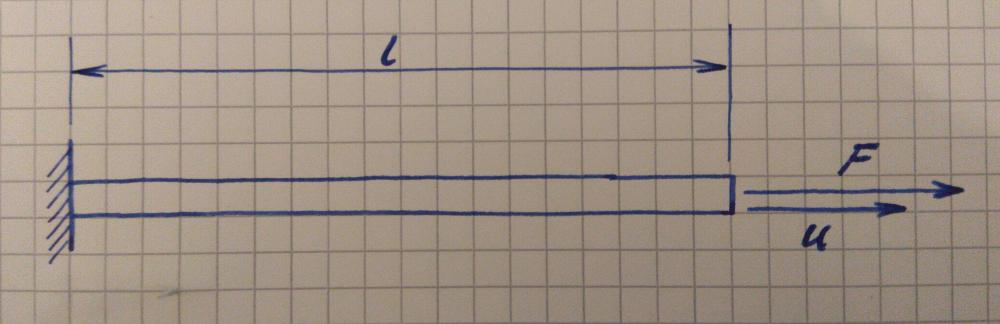
\includegraphics[width=0.5\textwidth]{figures/elements/castigliano-bar-1.jpg}
\caption{Bar of length $l$ with a load $F$ at the end}
\label{fig:castigliano-bar-1}
\end{figure}

First of all, the strain energy of a bar is given by

\begin{equation}
\Pi = \frac{1}{2}\int_{0}^{l}\frac{N^2}{EA}\,ds
\end{equation}

where $N(s)$ is the normal force of the cross sections along the length of the bar.
In this case it is easy to see that we have a constant normal force of $N(s) = F$.
According to Castigliano's theorem, the displacement $u$ in the direction of the force is

\begin{equation}
u = \frac{\partial \Pi}{\partial F} = \frac{\partial}{\partial F}\left(\frac{1}{2}\int_{0}^{l}\frac{F^2}{EA}\,ds\right) = \underbrace{\left(\int_{0}^{l}\frac{1}{EA}\,ds\right)}_{K^{-1}}F.
\end{equation}

By this we have identified the inverse $K^{-1}$ of the stiffness of the bar at that point and direction.
It is an integral over the length of the bar that takes the exact distribution of longitudinal stiffness into account.
If we assume $EA$ as constant for a quick sanity check, we get a stiffness of $K = \frac{EA}{l}$, which is the well known result for the stiffness of a bar.

It is especially worth mentioning that we arrived at this result without any kinematic considerations, i.e. we didn't have to think about the distribution of strain in the bar due to the normal force and how that relates to the displacement $u$, which makes the method very simple and elegant.
One apparent shortcoming of the method is that it only gives us the displacement at the end of the bar, where the external force is applied, and nowhere else.
This limitation can be worked around by introducing additional "imaginary" forces at other points of interest and setting them to zero after having calculated the associated displacements.

As part two of this exercise, let's calculate the displacement $\overline{u}$ at an arbitrary point $\overline{s}$ within the bar as shown in figure \ref{fig:castigliano-bar-2} by introducing the imaginary auxiliary force $\overline{F} = 0$.

\begin{figure}[h]
\centering
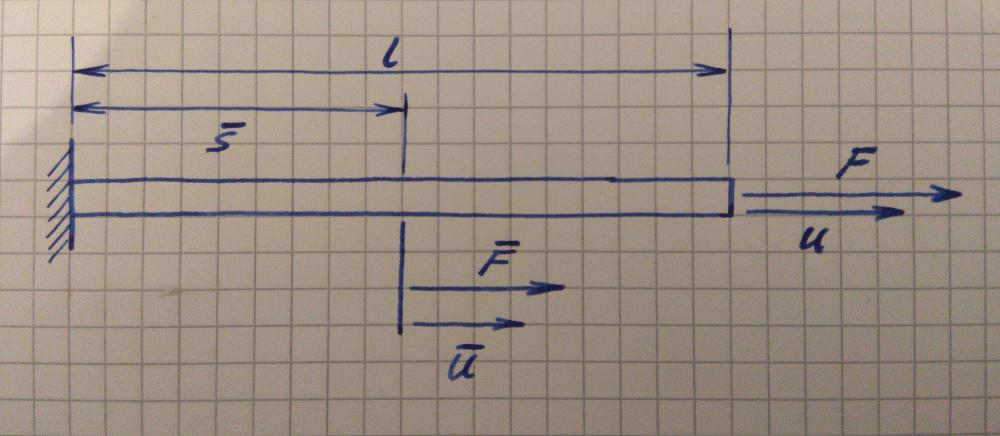
\includegraphics[width=0.5\textwidth]{figures/elements/castigliano-bar-2.jpg}
\caption{Bar of length $l$ with a load $F$ at the end and auxiliary force $\overline{F}$}
\label{fig:castigliano-bar-2}
\end{figure}

First of all, the distribution of normal force is now given by the piecewise function

\begin{equation}
N(s) = \begin{cases}
F + \overline{F}, & \text{if}\ \ 0 \le s < \overline{s} \\
F, & \text{if}\ \ \overline{s} \le s \le l \\
\end{cases}
\end{equation}

Therefore the potential elastic energy becomes
%
\begin{align}
\Pi &= \frac{1}{2}\int_{0}^{l}\frac{N^2}{EA}\,ds = \frac{1}{2}\left(\int_{0}^{\overline{s}}\frac{(F + \overline{F})^2}{EA}\,ds + \int_{\overline{s}}^{l}\frac{F^2}{EA}\,ds\right) \\
\end{align}

Application of Castigliano's theorem yields the displacement $\overline{u}$ depending on the forces $F$ and $\overline{F}$.
The actual displacement is obtained by setting the auxiliary force $\overline{F}$ to zero.
%
\begin{align}
\overline{u} &= \frac{\partial \Pi}{\partial \overline{F}} = \frac{\partial}{\partial \overline{F}}\left( \frac{1}{2} \int_{0}^{\overline{s}}\frac{(F + \overline{F})^2}{EA}\,ds \right) = \left(\int_{0}^{\overline{s}}\frac{1}{EA}\,ds \right)\left(F + \overline{F}\right) \\
&= \left(\int_{0}^{\overline{s}}\frac{1}{EA}\,ds \right)F.
\end{align}

This way we got the complete displacement distribution within the bar.
In the next section we are going to use Castigliano's theorem for calculating the stiffness matrix and displacements of a linear-elastic beam segment.

\newpage
\subsection{Stiffness Matrix of a Beam Segment (3)}

\begin{figure}[h]
\centering
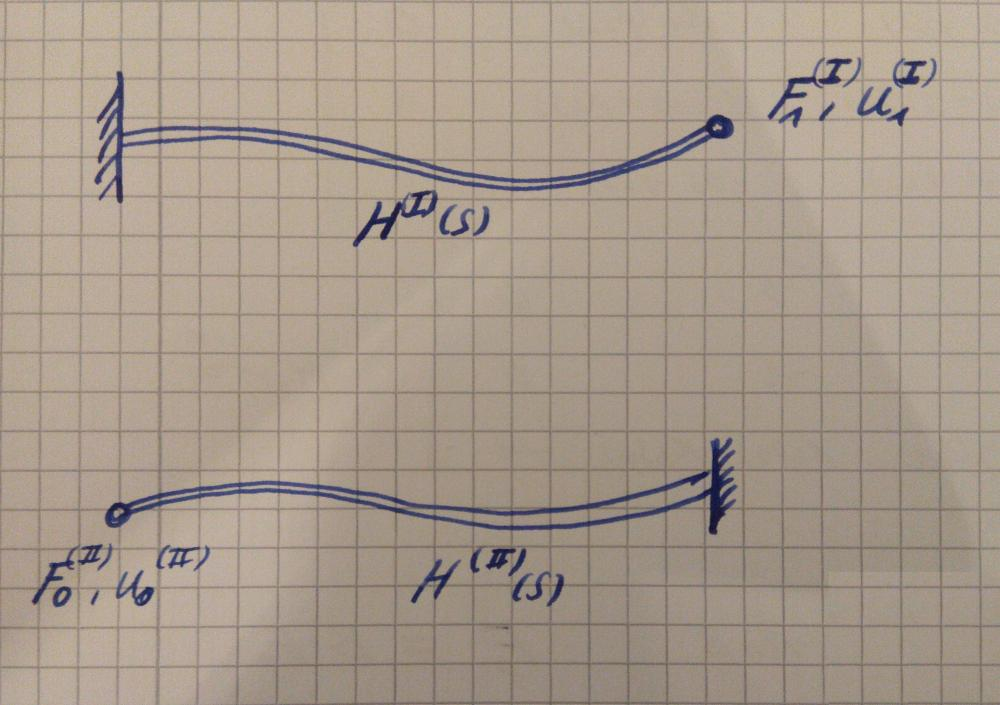
\includegraphics[width=0.5\textwidth]{figures/elements/castigliano-beam-cases.jpg}
\caption{Loading cases I and II}
\label{fig:castigliano-beam-cases}
\end{figure}

\subsubsection*{Loadcases}

The stiffness of the beam segment with respect to the combined nodal displacement and forces is

\begin{equation}
\underbrace{
\begin{bmatrix}
\boldsymbol{F}_0 \\
\boldsymbol{F}_1 \\
\end{bmatrix}
}_{\boldsymbol{F}}
=
\underbrace{
\begin{bmatrix}
\boldsymbol{K}_{0,0} & \boldsymbol{K}_{0,1} \\
\boldsymbol{K}_{1,0} & \boldsymbol{K}_{1,1} \\
\end{bmatrix}
}_{\boldsymbol{K}}
\underbrace{
\begin{bmatrix}
\boldsymbol{u}_0 \\
\boldsymbol{u}_1 \\
\end{bmatrix}
}_{\boldsymbol{u}}
\end{equation}

with the stiffness matrix $\boldsymbol{K} \in \mathbb{R}^{6 \times 6}$ and the four submatrices $\boldsymbol{K}_{ij} \in \mathbb{R}^{3 \times 3}$.
We can get a physical interpretation of the submatrices by constraining one of the nodes, ie. $\boldsymbol{u}_{0} = 0$ and $\boldsymbol{u}_{1} = 0$.

In the case $\boldsymbol{u}_{0} = 0$, which we will call case I, the resulting forces are

\begin{align}
\boldsymbol{F}_1 &= \boldsymbol{K}_{1,1}\,\boldsymbol{u}_1 \\
\boldsymbol{F}_0 &= \boldsymbol{K}_{0,1}\,\boldsymbol{u}_1
\end{align}

In the case $\boldsymbol{u}_{1} = 0$, which we will call case II, the resulting forces are

\begin{align}
\boldsymbol{F}_0 &= \boldsymbol{K}_{0,0}\,\boldsymbol{u}_0 \\
\boldsymbol{F}_1 &= \boldsymbol{K}_{1,0}\,\boldsymbol{u}_0
\end{align}

Put into words, the diagonal matrix blocks $\boldsymbol{K}_{0,0}$ and $\boldsymbol{K}_{1,1}$ relate the forces and displacements at a free node to each other, if the other node is restrained.
The off-diagonal blocks $\boldsymbol{K}_{1,0}$ and $\boldsymbol{K}_{0,1}$ relate the displacements at the free node to the forces at the restrained node.
This means that we can obtain the full stiffness matrix of the segment by analyzing those two distinct loadcases and assembling the partial results in the end.

The nodal forces $\boldsymbol{F}_0$ and $\boldsymbol{F}_1$ are not completely independent of each other, since they have to be in static equilibrium with each as a necessary condition for the element to be in equilibrium.
Balancing the forces and moments around node 1 gives us the three conditions
%
\begin{align}
x:\quad &F_{x,0} + F_{x,1} = 0 \\
y:\quad &F_{y,0} + F_{y,1} = 0 \\
z:\quad &M_{z,0} + M_{z,1} + F_{x,0}(y_1 - y_0) - F_{y,0}(x_1 - x_0) = 0
\end{align}

This can be written as the following matrix equation between the nodal forces,
%
\begin{align}
\boldsymbol{F}_0 &= \boldsymbol{B}_{0,1}\cdot\boldsymbol{F}_1 \\
\boldsymbol{F}_1 &= \boldsymbol{B}_{1,0}\cdot\boldsymbol{F}_0
\end{align}

with the matrix $\boldsymbol{B}_{i,j}$ defined as

\begin{equation}
\boldsymbol{B}_{i,j} = \begin{bmatrix}
-1 & 0 & 0 \\
0 & -1 & 0 \\
y_j - y_i & x_i - x_j & -1
\end{bmatrix}.
\end{equation}

We can use this relationship to calculate the forces at the clamped nodes in the cases I and II in order to obtain the off-diagonal stiffnesses $\boldsymbol{K}_{1,0}$ and $\boldsymbol{K}_{0,1}$ as follows,
%
\begin{align}
\boldsymbol{F}_0 &= \boldsymbol{B}_{0,1}\boldsymbol{F}_1 = \underbrace{\boldsymbol{B}_{0,1}\boldsymbol{K}_{1,1}}_{\boldsymbol{K}_{0,1}}\boldsymbol{u}_1 \\
\boldsymbol{F}_1 &= \boldsymbol{B}_{1,0}\boldsymbol{F}_0 = \underbrace{\boldsymbol{B}_{1,0}\boldsymbol{K}_{0,0}}_{\boldsymbol{K}_{1,0}}\boldsymbol{u}_0
\end{align}

In practive we only have to calculate one of the off-diagonal blocks since the complete stiffness matrix must be symmetric and therefore $\boldsymbol{K}_{1,0} = \boldsymbol{K}_{0,0}^\intercal$.
Since the off-diagonal stiffnesses have been shown to depend on the diagonal stiffnesses $\boldsymbol{K}_{0,0}$ and $\boldsymbol{K}_{1,1}$, the remaining task is to determine those matrices by analyzing the loadcases I and II, respectively.

\subsubsection*{Loadcase I}

The beam is clamped on the left and a force is applied at node 1.
Due to static equilibrium, the cross section forces in the beam for a force $\boldsymbol{F}_\eta$ that is applied at the length $s_\eta$ with $\eta \in [0,\,1]$ are

\begin{equation}
\underbrace{
\begin{bmatrix}
N \\ M \\ Q
\end{bmatrix}
}_{\boldsymbol{f}^{\mathrm{I}}_{\eta}(s)}
=
\underbrace{
\begin{bmatrix}
\cos(\varphi(s)) & \sin(\varphi(s)) & 0 \\
y(s) - y(s_\eta) & x(s_\eta) - x(s) & 1 \\
-\sin(\varphi(s)) & \cos(\varphi(s)) & 0 \\
\end{bmatrix}
}_{\boldsymbol{H}_{\eta}(s)}
\underbrace{
\begin{bmatrix}
F_{x,\eta} \\ F_{y,\eta} \\ M_{z,\eta}
\end{bmatrix}
}_{\boldsymbol{F}_\eta}. \label{eq:section-static-equilibrium}
\end{equation}

Combining the nodal force $\boldsymbol{F}_1$ at $s_1$ and the variable auxiliary force $\boldsymbol{F}_\eta$ at $s_\eta$:

\begin{equation}
\boldsymbol{f}^{\mathrm{I}}(s) = \begin{cases}
\boldsymbol{H}_{1}(s)\boldsymbol{F}_1 + \boldsymbol{H}_{\eta}(s)\boldsymbol{F}_\eta, & \text{if}\ \ s_0 \le s < s_\eta \\
\boldsymbol{H}_{1}(s)\boldsymbol{F}_1, & \text{if}\ \ s_\eta \le s \le s_1 \\
\end{cases}
\end{equation}

The potential energy for this loadcase is therefore

\begin{equation}
\Pi^{\mathrm{I}} = \frac{1}{2}\left(\int_{s_0}^{s_\eta} \left(\boldsymbol{H}_{1}\boldsymbol{F}_1 + \boldsymbol{H}_{\eta}\boldsymbol{F}_\eta\right)^\intercal\boldsymbol{C}^{-1}\left(\boldsymbol{H}_{1}\boldsymbol{F}_1 + \boldsymbol{H}_{\eta}\boldsymbol{F}_\eta\right)\,ds + \int_{s_\eta}^{s_1} \left(\boldsymbol{H}_{1}\boldsymbol{F}_1\right)^\intercal\boldsymbol{C}^{-1}\left(\boldsymbol{H}_{1}\boldsymbol{F}_1\right)\,ds\right)
\end{equation}

and the displacement $\boldsymbol{u}_\eta$ at position $s_\eta$

\begin{align}
\boldsymbol{u}^{\mathrm{I}}_\eta &= \frac{\partial \Pi^{\mathrm{I}}}{\partial \boldsymbol{F}_\eta}\Bigg|_{\boldsymbol{F}_\eta = 0} = \frac{\partial}{\partial \boldsymbol{F}_\eta}\left(\frac{1}{2}\int_{s_0}^{s_\eta} \left(\boldsymbol{H}_{1}\boldsymbol{F}_1 + \boldsymbol{H}_{\eta}\boldsymbol{F}_e\right)^\intercal\boldsymbol{C}^{-1}\left(\boldsymbol{H}_{1}\boldsymbol{F}_1 + \boldsymbol{H}_{\eta}\boldsymbol{F}_\eta\right)\,ds\right)\Bigg|_{\boldsymbol{F}_\eta = 0} \notag \\
&= \underbrace{\left(\int_{s_0}^{s_\eta} \boldsymbol{H}_\eta^\intercal\boldsymbol{C}^{-1}\boldsymbol{H}_1\,ds\right)}_{\boldsymbol{K}^{-1}_{1,\eta}}\boldsymbol{F}_1
\end{align}

The stiffness matrix $\boldsymbol{K}^{-1}_{1,1}$ for the right node follows for $\eta = 1$.

%Displacement at node 1 ($s_e = s_1$):
%
%\begin{align}
%\boldsymbol{u}^{(I)}_1 &= \underbrace{\left(\int_{s_0}^{s_e} \boldsymbol{H}_1^\intercal\boldsymbol{C}^{-1}\boldsymbol{H}_1\,ds\right)}_{\boldsymbol{K}^{-1}_{1,1}}\boldsymbol{F}_1
%\end{align}

\subsubsection*{Loadcase II}

\begin{equation}
\underbrace{
\begin{bmatrix}
N \\ M \\ Q
\end{bmatrix}
}_{\boldsymbol{f}^{\mathrm{II}}_{\eta}(s)}
=
\underbrace{
\begin{bmatrix}
-\cos(\varphi(s)) & -\sin(\varphi(s)) & 0 \\
y(s_\eta) - y(s) & x(s) - x(s_\eta) & -1 \\
\sin(\varphi(s)) & -\cos(\varphi(s)) & 0 \\
\end{bmatrix}
}_{-\boldsymbol{H}_{\eta}(s)}
\underbrace{
\begin{bmatrix}
F_{x,\eta} \\ F_{y,\eta} \\ M_{z,\eta}
\end{bmatrix}
}_{\boldsymbol{F}_\eta}. \label{eq:section-static-equilibrium}
\end{equation}

\begin{equation}
\boldsymbol{f}^{\mathrm{II}}(s) = \begin{cases}
-\boldsymbol{H}_{0}(s)\boldsymbol{F}_0, & \text{if}\ \ s_0 \le s \le s_\eta \\
-\boldsymbol{H}_{0}(s)\boldsymbol{F}_0 - \boldsymbol{H}_{\eta}(s)\boldsymbol{F}_\eta, & \text{if}\ \ s_\eta \le s < s_1 \\
\end{cases}
\end{equation}

\begin{equation}
\Pi^{\mathrm{II}} = \frac{1}{2}\left(\int_{s_0}^{s_\eta} \left(\boldsymbol{H}_{0}\boldsymbol{F}_0\right)^\intercal\boldsymbol{C}^{-1}\left(\boldsymbol{H}_{0}\boldsymbol{F}_0\right)\,ds + \int_{s_\eta}^{s_1} \left(\boldsymbol{H}_{0}\boldsymbol{F}_0 + \boldsymbol{H}_{\eta}\boldsymbol{F}_\eta\right)^\intercal\boldsymbol{C}^{-1}\left(\boldsymbol{H}_{0}\boldsymbol{F}_0 + \boldsymbol{H}_{\eta}\boldsymbol{F}_\eta\right)\,ds\right)
\end{equation}

\begin{align}
\boldsymbol{u}^{\mathrm{II}}_\eta &= \frac{\partial \Pi^{\mathrm{II}}}{\partial \boldsymbol{F}_\eta}\Bigg|_{\boldsymbol{F}_\eta = 0} = \frac{\partial}{\partial \boldsymbol{F}_\eta}\left(\frac{1}{2}\int_{s_\eta}^{s_1} \left(\boldsymbol{H}_{0}\boldsymbol{F}_0 + \boldsymbol{H}_{\eta}\boldsymbol{F}_\eta\right)^\intercal\boldsymbol{C}^{-1}\left(\boldsymbol{H}_{0}\boldsymbol{F}_0 + \boldsymbol{H}_{\eta}\boldsymbol{F}_\eta\right)\,ds\right)\Bigg|_{\boldsymbol{F}_\eta = 0} \notag \\
&= \underbrace{\left(\int_{s_\eta}^{s_1} \boldsymbol{H}_\eta^\intercal\boldsymbol{C}^{-1}\boldsymbol{H}_0\,ds\right)}_{\boldsymbol{K}^{-1}_{0,\eta}}\boldsymbol{F}_0
\end{align}

The stiffness matrix $\boldsymbol{K}^{-1}_{0,0}$ for the left node follows for $\eta = 0$.

%Displacement at node 1 ($s_e = s_1$):
%
%\begin{align}
%\boldsymbol{u}^{(II)}_0 &= \underbrace{\left(\int_{s_e}^{s_1} \boldsymbol{H}_0^\intercal\boldsymbol{C}^{-1}\boldsymbol{H}_0\,ds\right)}_{\boldsymbol{K}^{-1}_{0,0}}\boldsymbol{F}_0
%\end{align}

\subsubsection*{Combined Displacements}

Due to linear superposition \textcolor{red}{TODO: explain}, the displacements under forces at both nodes can be added as

\begin{equation}
\boldsymbol{u}_{\eta} = \boldsymbol{K}_{0,\eta}^{-1}\,\boldsymbol{F}_0 + \boldsymbol{K}_{1,\eta}^{-1}\,\boldsymbol{F}_1.
\end{equation}

Therefore the displacement evaluation matrix is

\begin{align}
\boldsymbol{u}_{\eta} &= \boldsymbol{K}_{0,\eta}^{-1}\boldsymbol{K}_{0,0}\boldsymbol{u}_0 + \boldsymbol{K}_{1,\eta}^{-1}\boldsymbol{K}_{1,1}\boldsymbol{u}_1 \\
&=
\underbrace{
\left[\boldsymbol{K}_{0,\eta}^{-1}\boldsymbol{K}_{0,0} \ \vert\ \boldsymbol{K}_{1,\eta}^{-1}\boldsymbol{K}_{1,1}\right]
}_{\boldsymbol{U}_\eta}
\begin{bmatrix}
\boldsymbol{u}_0 \notag \\
\boldsymbol{u}_1
\end{bmatrix} \notag \\
&=\boldsymbol{U}_\eta\boldsymbol{u}
\end{align}

We can simplify the computation of the matrices $\boldsymbol{K}_{0,\eta}^{-1}$ and $\boldsymbol{K}^{-1}_{1,\eta}$ by realizing that $\boldsymbol{H}_0$ and $\boldsymbol{H}_1$ are related by the static equilibrium matrix $\boldsymbol{B}_{i,j}$ \textcolor{red}{TODO: Link} as

\begin{equation}
\boldsymbol{H}_\eta(s) = -\boldsymbol{H}_0(s)\boldsymbol{B}_{\eta,0}
\end{equation}

This way, the flexibility matrices can be written as
%
\begin{align}
\boldsymbol{K}_{0,\eta}^{-1} &= -\boldsymbol{B}_{0,\eta}^\intercal\left(\int_{s_\eta}^{s_1} \boldsymbol{H}_0^\intercal\boldsymbol{C}^{-1}\boldsymbol{H}_0\,ds\right) \\
\boldsymbol{K}^{-1}_{1,\eta} &= \boldsymbol{B}_{0,\eta}^\intercal\left(\int_{s_0}^{s_\eta} \boldsymbol{H}_0^\intercal\boldsymbol{C}^{-1}\boldsymbol{H}_0\,ds\right)\boldsymbol{B}_{0,1}
\end{align}

so now there is only one function to be integrated, even though over different bounds, and the matrices for different $\eta$ are obtained by multiplying with the $\boldsymbol{B}$ matrices.
In the implementation, the integrand can be evaluated for each sub-interval between $s_0$ and $s_1$ and the partial results can be added as needed. \textcolor{red}{Better explanation?}

\subsubsection*{Combined Forces}

\begin{align}
\boldsymbol{f}(s) &= \boldsymbol{f}^{\mathrm{I}}(s) + \boldsymbol{f}^{\mathrm{II}}(s) \notag \\
&= \boldsymbol{H}_{1}(s)\boldsymbol{F}_1 - \boldsymbol{H}_{0}(s)\boldsymbol{F}_0 \notag \\
&= \begin{bmatrix}
-\boldsymbol{H}_{0}(s), & \boldsymbol{H}_{1}(s)
\end{bmatrix}
\boldsymbol{F} \notag \\
&= \begin{bmatrix}
-\boldsymbol{H}_{0}(s), & \boldsymbol{H}_{1}(s)
\end{bmatrix}
\boldsymbol{K}\boldsymbol{u} \notag \\
&= \begin{bmatrix}
\boldsymbol{H}_{1}\boldsymbol{K}_{1,0} - \boldsymbol{H}_{0}\boldsymbol{K}_{0,0}, & \boldsymbol{H}_{1}\boldsymbol{K}_{1,1} - \boldsymbol{H}_{0}\boldsymbol{K}_{0,1}
\end{bmatrix}\boldsymbol{u} \notag \\
\end{align}

%\newpage
%\subsection{Stiffness Matrix of a Beam Segment (2)}
%
%\subsubsection{Case I}
%
%Section forces when force $\boldsymbol{F}_e$ is applied at point $s_e$:
%
%\begin{equation}
%\underbrace{
%\begin{bmatrix}
%N \\ M \\ Q
%\end{bmatrix}
%}_{\boldsymbol{f}_e(s)}
%=
%\underbrace{
%\begin{bmatrix}
%\cos(\varphi(s)) & \sin(\varphi(s)) & 0 \\
%y(s) - y(s_e) & x(s_e) - x(s) & 1 \\
%-\sin(\varphi(s)) & \cos(\varphi(s)) & 0 \\
%\end{bmatrix}
%}_{\boldsymbol{H}_{e}(s)}
%\underbrace{
%\begin{bmatrix}
%F_{xe} \\ F_{ye} \\ M_{ze}
%\end{bmatrix}
%}_{\boldsymbol{F}_e}, \quad s \in [0,\,s_e]. \label{eq:section-static-equilibrium}
%\end{equation}
%
%Force $\boldsymbol{F}_1$ at $s_1$ and auxiliary force $\boldsymbol{F}_e$ at $s_e$:
%
%\begin{equation}
%\boldsymbol{f}^{(I)}(s) = \begin{cases}
%\boldsymbol{H}_{1}(s)\boldsymbol{F}_1 + \boldsymbol{H}_{e}(s)\boldsymbol{F}_e, & \text{if}\ \ s_0 \le s < s_e \\
%\boldsymbol{H}_{1}(s)\boldsymbol{F}_1, & \text{if}\ \ s_e \le s \le s_1 \\
%\end{cases}
%\end{equation}
%
%Elastic energy for case I:
%
%\begin{equation}
%\Pi^{(I)} = \frac{1}{2}\left(\int_{s_0}^{s_e} \left(\boldsymbol{H}_{1}\boldsymbol{F}_1 + \boldsymbol{H}_{e}\boldsymbol{F}_e\right)^\intercal\boldsymbol{C}^{-1}\left(\boldsymbol{H}_{1}\boldsymbol{F}_1 + \boldsymbol{H}_{e}\boldsymbol{F}_e\right)\,ds + \int_{s_e}^{s_1} \left(\boldsymbol{H}_{1}\boldsymbol{F}_1\right)^\intercal\boldsymbol{C}^{-1}\left(\boldsymbol{H}_{1}\boldsymbol{F}_1\right)\,ds\right)
%\end{equation}
%
%\begin{align}
%\boldsymbol{u}^{(I)}_e &= \frac{\partial \Pi^{(I)}}{\partial \boldsymbol{F}_e}\Bigg|_{\boldsymbol{F}_e = 0} = \frac{\partial}{\partial \boldsymbol{F}_e}\left(\frac{1}{2}\int_{s_0}^{s_e} \left(\boldsymbol{H}_{1}\boldsymbol{F}_1 + \boldsymbol{H}_{e}\boldsymbol{F}_e\right)^\intercal\boldsymbol{C}^{-1}\left(\boldsymbol{H}_{1}\boldsymbol{F}_1 + \boldsymbol{H}_{e}\boldsymbol{F}_e\right)\,ds\right)\Bigg|_{\boldsymbol{F}_e = 0} \notag \\
%&= \underbrace{\left(\int_{s_0}^{s_e} \boldsymbol{H}_e^\intercal\boldsymbol{C}^{-1}\boldsymbol{H}_1\,ds\right)}_{\boldsymbol{K}^{-1}_{1,e}}\boldsymbol{F}_1
%\end{align}
%
%Displacement at node 1 ($s_e = s_1$):
%
%\begin{align}
%\boldsymbol{u}^{(I)}_1 &= \underbrace{\left(\int_{s_0}^{s_e} \boldsymbol{H}_1^\intercal\boldsymbol{C}^{-1}\boldsymbol{H}_1\,ds\right)}_{\boldsymbol{K}^{-1}_{1,1}}\boldsymbol{F}_1
%\end{align}
%
%\newpage
%\subsubsection{Case II}
%
%Force $\boldsymbol{F}_0$ at $s_0$ and auxiliary force $\boldsymbol{F}_e$ at $s_e$: Can be derived from $\Pi^{(I)}$ by setting $\boldsymbol{F}_1 = \boldsymbol{B}\boldsymbol{F}_0$:
%
%\begin{equation}
%\boldsymbol{f}^{(II)}(s) = \begin{cases}
%\boldsymbol{H}_{1}(s)\boldsymbol{F}_1 + \boldsymbol{H}_{e}(s)\boldsymbol{F}_e, & \text{if}\ \ s_0 \le s < s_e \\
%\boldsymbol{H}_{1}(s)\boldsymbol{F}_1, & \text{if}\ \ s_e \le s \le s_1 \\
%\end{cases}
%\end{equation}
%
%
%
%\begin{equation}
%\Pi^{(II)} = \frac{1}{2}\left(\int_{s_0}^{s_e} \left(\boldsymbol{H}_{1}\boldsymbol{B}\boldsymbol{F}_0 + \boldsymbol{H}_{e}\boldsymbol{F}_e\right)^\intercal\boldsymbol{C}^{-1}\left(\boldsymbol{H}_{1}\boldsymbol{B}\boldsymbol{F}_0 + \boldsymbol{H}_{e}\boldsymbol{F}_e\right)\,ds + \int_{s_e}^{s_1} \left(\boldsymbol{H}_{1}\boldsymbol{B}\boldsymbol{F}_0\right)^\intercal\boldsymbol{C}^{-1}\left(\boldsymbol{H}_{1}\boldsymbol{B}\boldsymbol{F}_0\right)\,ds\right)
%\end{equation}
%
%(Wrong derivation, final result is a conjecture...)
%
%\begin{align}
%\boldsymbol{u}^{(II)}_e &= \frac{\partial \Pi^{(II)}}{\partial \boldsymbol{F}_e}\Bigg|_{\boldsymbol{F}_e = 0} = \frac{\partial}{\partial \boldsymbol{F}_e}\left(\frac{1}{2}\int_{s_0}^{s_e} \left(\boldsymbol{H}_{1}\boldsymbol{B}\boldsymbol{F}_0 + \boldsymbol{H}_{e}\boldsymbol{F}_e\right)^\intercal\boldsymbol{C}^{-1}\left(\boldsymbol{H}_{1}\boldsymbol{B}\boldsymbol{F}_0 + \boldsymbol{H}_{e}\boldsymbol{F}_e\right)\,ds\right)\Bigg|_{\boldsymbol{F}_e = 0} \notag \\
%&= \underbrace{\left(\int_{s_0}^{s_e} \boldsymbol{H}_e^\intercal\boldsymbol{C}^{-1}\boldsymbol{H}_1\,ds\right)\boldsymbol{B}}_{\boldsymbol{K}^{-1}_{1,e}}\boldsymbol{F}_1
%\end{align}
%
%Displacement at node 0 ($s_e = s_0$):
%
%\begin{align}
%\boldsymbol{u}^{(II)}_0 &= \underbrace{\left(\int_{s_0}^{s_e} \boldsymbol{H}_1^\intercal\boldsymbol{C}^{-1}\boldsymbol{H}_1\,ds\right)}_{\boldsymbol{K}^{-1}_{1,1}}\boldsymbol{F}_1
%\end{align}

\newpage
\subsection{Stiffness Matrix of a Beam Segment}

In this section we will derive the analytical stiffness matrix for a curved beam segment with arbitrary cross section properties that is also shear-deformable.
The only assumption we will make is that all displacements are small, so that we can apply linear-elastic theory to the problem.

\begin{figure}[h]
\centering
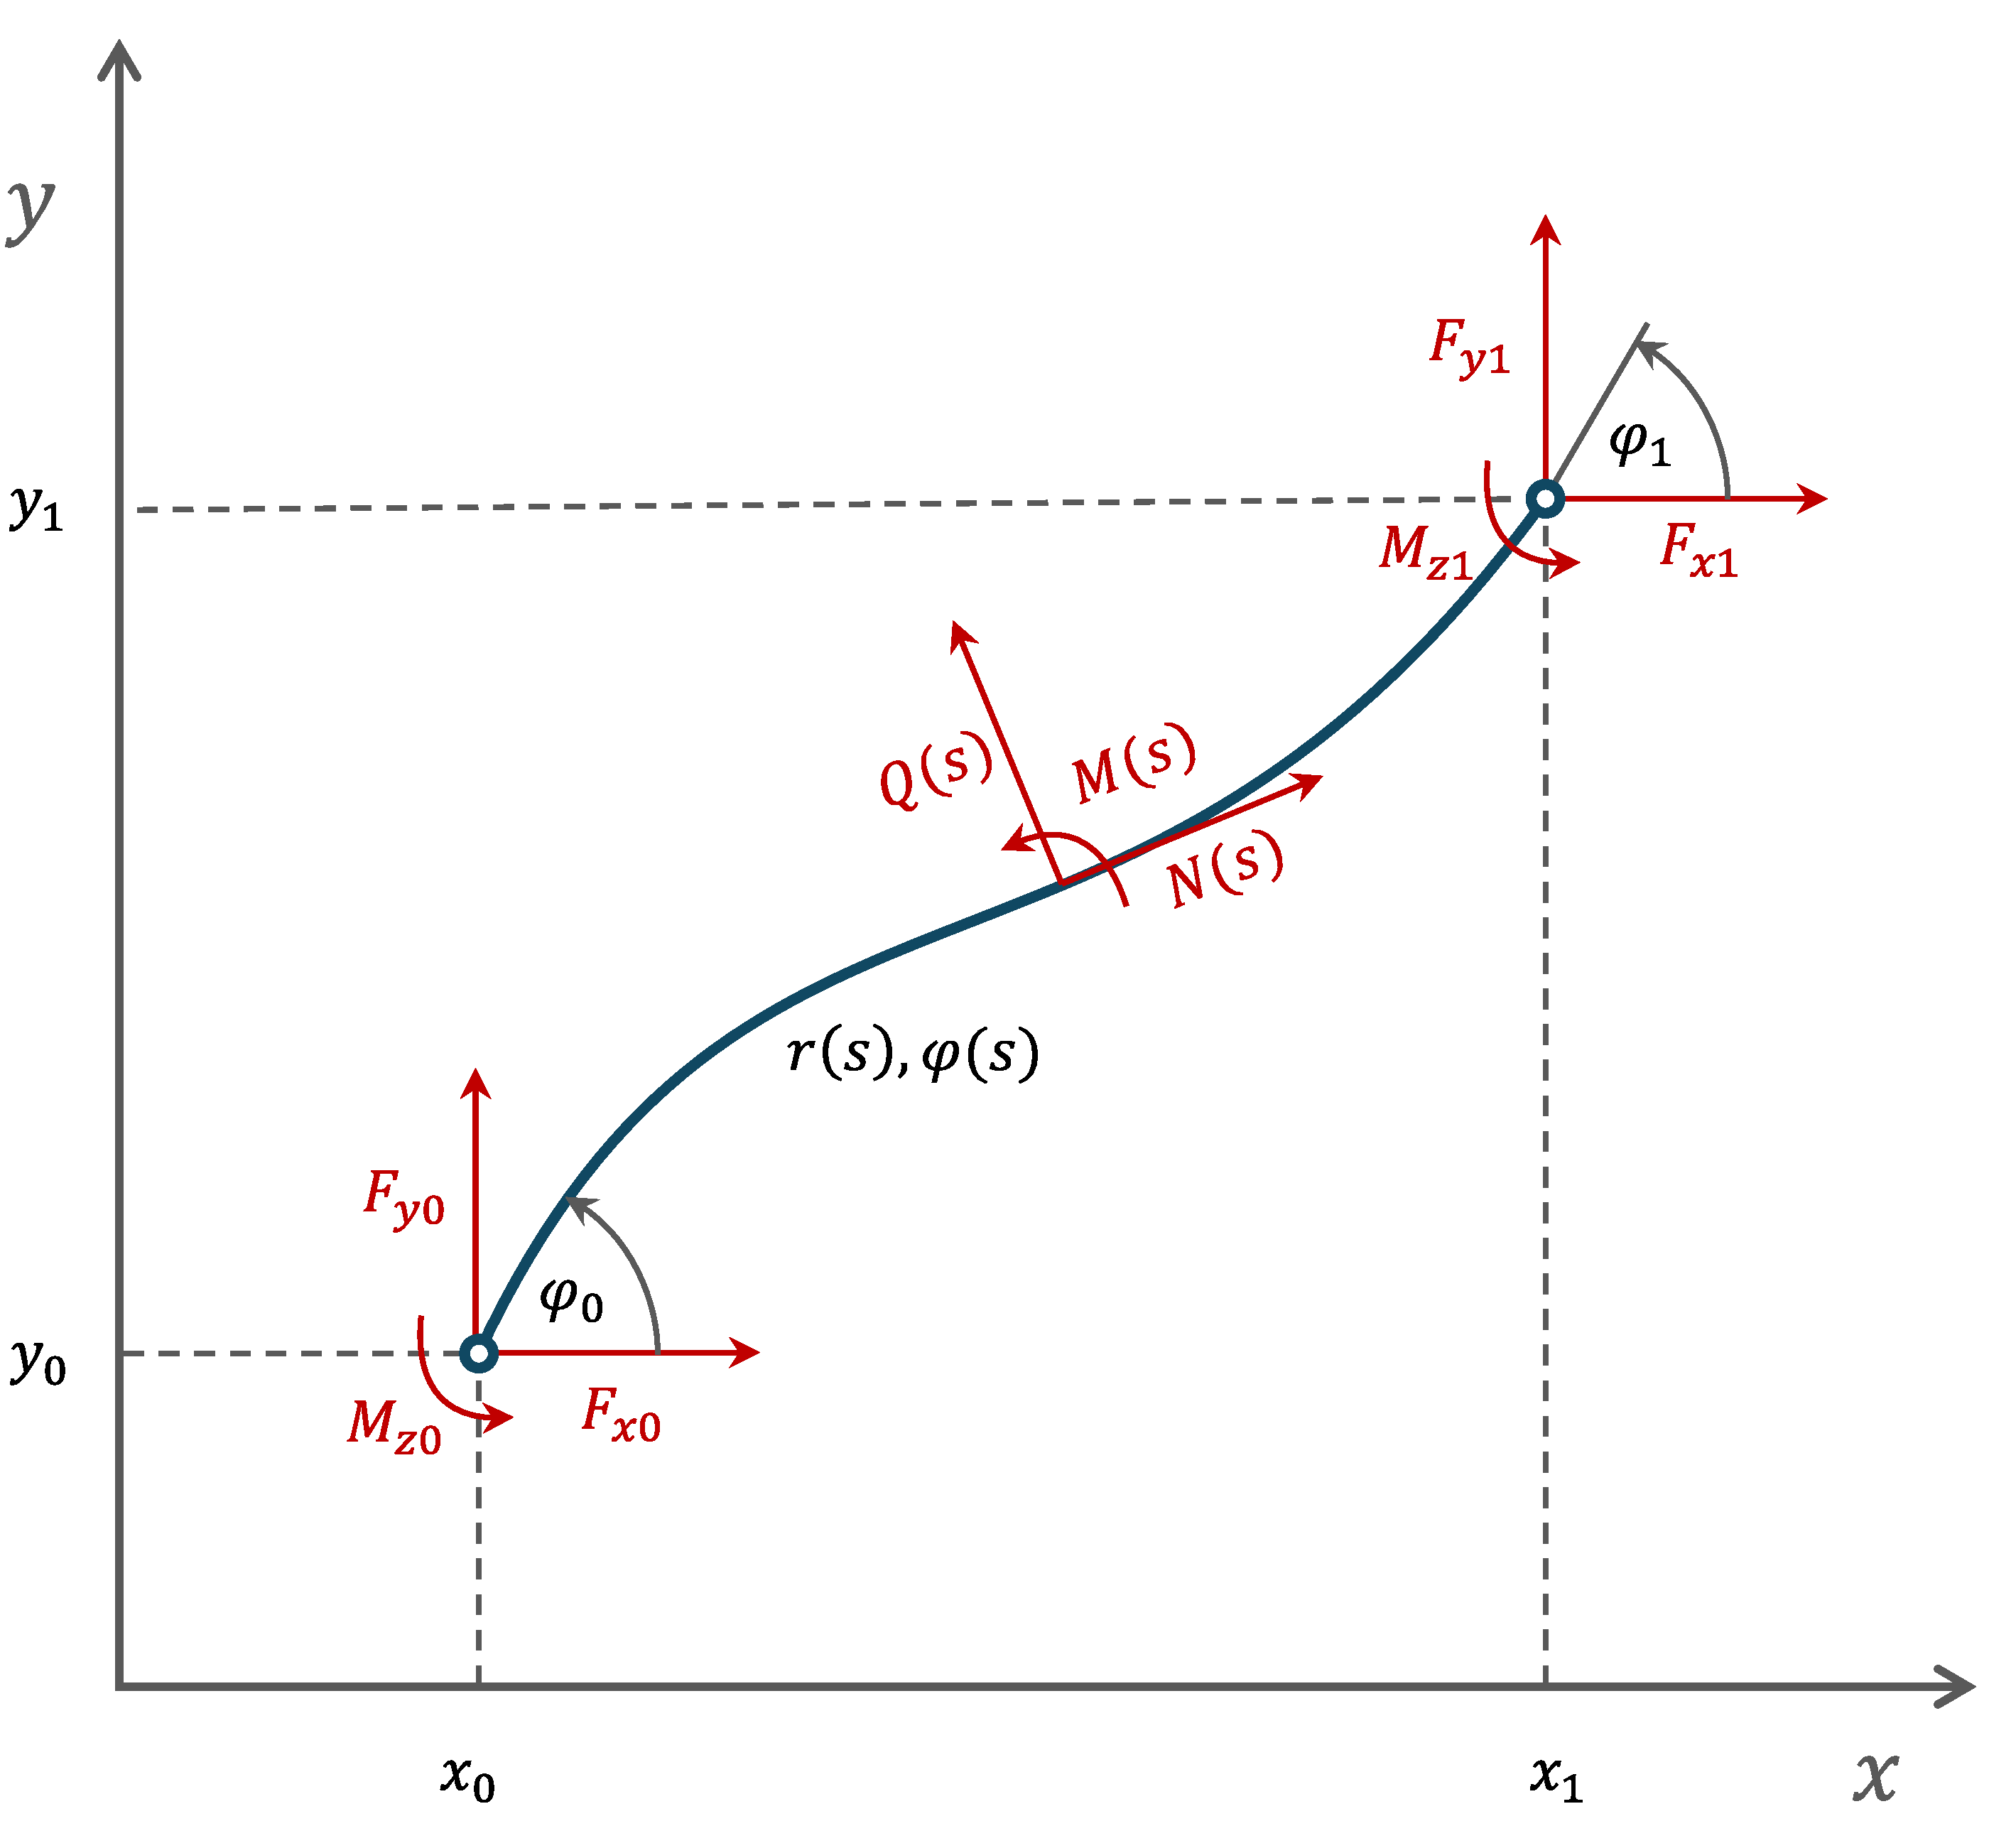
\includegraphics[width=0.5\textwidth]{figures/elements/beam-segment-linear}
\caption{Arbitrary beam segment with two nodes}
\label{fig:beam-segment-linear}
\end{figure}

Consider the beam segment shown in figure $\ref{fig:beam-segment-linear}$.
Its shape is described by the undeformed reference curve $\boldsymbol{r}(s) = \left[x(s),\,y(s)\right]^\intercal$ and the associated orientation angle $\varphi(s)$, where the parameter $s \in [s_0,\,s_1]$ is the arc length along the curve.

The stiffness properties of the cross sections are described by the cross sectional stiffness matrix $\boldsymbol{C}(s) \in \mathbb{R}^{3 \times 3}$ that is assumed to be known and establishes a linear constitutive relation of the form

\begin{equation}
\underbrace{
\begin{bmatrix}
N \\
M \\
Q \\
\end{bmatrix}
}_{\boldsymbol{f}(s)}
=
\underbrace{
\begin{bmatrix}
C_{\varepsilon\varepsilon} & C_{\varepsilon\kappa} & C_{\varepsilon\gamma} \\
C_{\varepsilon\kappa} & C_{\kappa\kappa} & C_{\kappa\gamma} \\
C_{\varepsilon\gamma} & C_{\kappa\gamma} & C_{\gamma\gamma} \\
\end{bmatrix}
}_{\boldsymbol{C}(s)}
\underbrace{
\begin{bmatrix}
\varepsilon \\
\kappa \\
\gamma \\
\end{bmatrix}
}_{\boldsymbol{e}(s)} \label{eq:section-stiffness-matrix}
\end{equation}

between the cross section forces~$\boldsymbol{f}$ and the generalized strains~$\boldsymbol{e}$.
The cross section forces consist of the normal force~$N$, the bending moment~$M$ and the shear force~$Q$ as shown in figure~\ref{fig:beam-segment-linear} while the strains consist of the elongation~$\varepsilon$ and the curvature~$\kappa$ of the beam axis as well as the shear angle~$\gamma$ between the section and the beam axis.

We assign two nodes to this segment, one on the starting point and one on the endpoint of the curve.
Each node is given two translational degrees of freedom in x- and y-direction and an angular degree of freedom around the z-axis.
At each node, the respective forces and moments

\begin{equation}
\boldsymbol{F}_{0} = \begin{bmatrix}
F_{x0} \\ F_{y0} \\ M_{z0}
\end{bmatrix},
\quad
\boldsymbol{F}_{1} = \begin{bmatrix}
F_{x1} \\ F_{y1} \\ M_{z1}
\end{bmatrix}
\end{equation}

are applied, to which the beam segment reacts with the (small) displacements

\begin{equation}
\boldsymbol{u}_{0} = \begin{bmatrix}
\Delta x_0 \\ \Delta y_0 \\ \Delta \varphi_0
\end{bmatrix},
\quad
\boldsymbol{u}_{1} = \begin{bmatrix}
\Delta x_1 \\ \Delta y_1 \\ \Delta \varphi_1
\end{bmatrix}
\end{equation}

in the respective directions of the forces/moments and relative to the initial state.
The goal is now to find the stiffness matrix of the segment, which describes the linear relationship between those forces and displacements.
We will do this by following the approach outlined in~\cite{bib:curved-beam-stiffness-matrix}, which is based on Castigliano's theorem, an energy-based method for calculating displacements of linear-elastic structures.

We start with a simple static consideration of the nodal forces.
In order for the segment to be in static equilibrium, the nodal forces have to fulfill the following conditions,
%
\begin{align}
x:\quad &F_{x0} + F_{x1} = 0 \\
y:\quad &F_{y0} + F_{y1} = 0 \\
z:\quad &M_{z0} + M_{z1} + F_{x0}\Delta y - F_{y0}\Delta x = 0
\end{align}

where~$\Delta x = x_1 - x_0$ and~$\Delta y = y_1 - y_0$.
This can be rearranged into a matrix equation that relates the forces on node 1 to those on node 0,

\begin{equation}
\underbrace{
\begin{bmatrix}
F_{x1} \\
F_{y1} \\
M_{z1} \\
\end{bmatrix}
}_{\boldsymbol{F}_1}
=
\underbrace{
\begin{bmatrix}
-1 & 0 & 0 \\
0 & -1 & 0 \\
-\Delta y & \Delta x & -1 \\
\end{bmatrix}
}_{\boldsymbol{B}}
\underbrace{
\begin{bmatrix}
F_{x0} \\
F_{y0} \\
M_{z0} \\
\end{bmatrix}
}_{\boldsymbol{F}_0}, \label{eq:segment-static-equilibrium}
\end{equation}

leaving only three independent nodal forces.
In a similar manner we can express the cross section forces $N(s)$, $M(s)$ and $Q(s)$ along the lenth of the segment in terms of the forces applied on node 1 by requiring the sections to be in static equilibrium with the applied forces.
This results in

\begin{equation}
\underbrace{
\begin{bmatrix}
N \\ M \\ Q
\end{bmatrix}
}_{\boldsymbol{f}(s)}
=
\underbrace{
\begin{bmatrix}
\cos(\varphi(s)) & \sin(\varphi(s)) & 0 \\
y(s) - y_1 & x_1 - x(s) & 1 \\
-\sin(\varphi(s)) & \cos(\varphi(s)) & 0 \\
\end{bmatrix}
}_{\boldsymbol{H}(s)}
\underbrace{
\begin{bmatrix}
F_{x1} \\ F_{y1} \\ M_{z1}
\end{bmatrix}
}_{\boldsymbol{F}_1}. \label{eq:section-static-equilibrium}
\end{equation}

Another prerequisite is the potential elastic energy (strain energy) of the beam segment.
It can be evaluated by integrating the product $\boldsymbol{f}^\intercal\boldsymbol{e}$ of section forces and strains over the beam's length and using the stiffness relation (\ref{eq:section-stiffness-matrix}) to eliminate the unknown strains:

\begin{equation}
\Pi = \frac{1}{2}\int_{s_0}^{s_1} \boldsymbol{f}^\intercal\boldsymbol{e}\,ds = \frac{1}{2}\int_{s_0}^{s_1} \boldsymbol{f}^\intercal\boldsymbol{C}^{-1}\boldsymbol{f}\,ds.
\end{equation}

According to Castigliano's second theorem, the partial derivative of the strain energy of a linear-elastic structure with respect to an applied force/moment is equal to the displacement/rotation of the structure at that point.

Let's first consider a load case where node 0 is fixed and forces are applied at node 1 only.
In this case, using equation (\ref{eq:section-static-equilibrium}), the strain energy becomes

\begin{equation}
\Pi_1 = \frac{1}{2}\int_{s_0}^{s_1} \boldsymbol{f}^\intercal\boldsymbol{C}^{-1}\boldsymbol{f}\,ds = \frac{1}{2}\boldsymbol{F}_1^\intercal\left(\int_{s_0}^{s_1} \boldsymbol{H}^\intercal\boldsymbol{C}^{-1}\boldsymbol{H}\,ds\right)\boldsymbol{F}_1
\end{equation}

and therefore, according to Castigliano's theorem, the corresponding displacements are

\begin{equation}
\boldsymbol{u}_{1} = \frac{\partial \Pi_1}{\partial \boldsymbol{F}_1} = \underbrace{\left(\int_{s_0}^{s_1} \boldsymbol{H}^\intercal\boldsymbol{C}^{-1}\boldsymbol{H}\,ds\right)}_{\boldsymbol{K}_{11}^{-1}}\boldsymbol{F}_1 = \boldsymbol{K}_{11}^{-1}\boldsymbol{F}_1.
\end{equation}

With this we have identified the inverse stiffness matrix $\boldsymbol{K}_{11}^{-1}$ that relates forces and displacements on node 1 to each other in this restricted load case.
Let's now consider the opposite case, where node 1 is fixed and the forces are applied at node 0 only.

Using (\ref{eq:section-static-equilibrium}) and (\ref{eq:segment-static-equilibrium}) we can express the strain energy in terms of $\boldsymbol{F}_0$ as

\begin{equation}
\Pi_0 = \frac{1}{2}\int_{s_0}^{s_1} \boldsymbol{f}^\intercal\boldsymbol{C}^{-1}\boldsymbol{f}\,ds = \frac{1}{2}\boldsymbol{F}_0^\intercal\underbrace{\boldsymbol{B}^\intercal\left(\int_{s_0}^{s_1} \boldsymbol{H}^\intercal\boldsymbol{C}^{-1}\boldsymbol{H}\,ds\right)\boldsymbol{B}}_{\boldsymbol{B}^\intercal\boldsymbol{K_{11}^{-1}\boldsymbol{B}}}\boldsymbol{F}_0.
\end{equation}

With the same reasoning as before this gives us the displacements

\begin{equation}
\boldsymbol{u}_{0} = \frac{\partial \Pi_0}{\partial \boldsymbol{F}_0} = \underbrace{\boldsymbol{B}^\intercal\boldsymbol{K_{11}^{-1}\boldsymbol{B}}}_{\boldsymbol{K}_{00}^{-1}}\boldsymbol{F}_0 = \boldsymbol{K}_{00}^{-1}\boldsymbol{F}_0
\end{equation}

and the inverse stiffness matrix $\boldsymbol{\boldsymbol{K}_{00}^{-1}}$ for node 0 in the considered configuration.
Since we are dealing with linear elasticity, we can use linear superposition of both of those load cases in order to get the overall stiffness relation of the beam segment.
We are however still missing the coupling between the nodes, i.e. the relationship between forces on node 0 and displacements on node 1 and vice versa.
For this we can use the static relationship~(\ref{eq:segment-static-equilibrium}) and the definition of the stiffness matrix to get
%
\begin{align}
\boldsymbol{F}_1 &= \boldsymbol{B}\boldsymbol{F}_0 = \underbrace{\boldsymbol{B}\boldsymbol{K}_{00}}_{\boldsymbol{K}_{10}}\boldsymbol{u}_0 = \boldsymbol{K}_{10}\boldsymbol{u}_0.
\end{align}

Due to symmetry we know that the second coupling stiffness must be $\boldsymbol{K}_{01} = \boldsymbol{K}_{10}^\intercal$.
Finally we add the forces from both load cases, which results in the complete stiffness relation for the beam segment as

\begin{equation}
\underbrace{
\begin{bmatrix}
\boldsymbol{F}_0 \\ \boldsymbol{F}_1
\end{bmatrix}
}_{\boldsymbol{F}}
=
\underbrace{
\begin{bmatrix}
\boldsymbol{K}_{00} & \boldsymbol{K}_{10}^\intercal \\
\boldsymbol{K}_{10} & \boldsymbol{K}_{11}
\end{bmatrix}
}_{\boldsymbol{K}}
\underbrace{
\begin{bmatrix}
\boldsymbol{u}_0 \\ \boldsymbol{u}_1
\end{bmatrix}
}_{\boldsymbol{u}} \label{eq:segment-stiffness-matrix}
\end{equation}

with the complete $6 \times 6$ stiffness matrix $\boldsymbol{K}$.
Note that this is an exact result since no simplifications have been made within the linear-elastic beam theory.
The integral over the beam length that occurs in the calculation of the partial stiffness matrices accounts for any arbitrary shape and distribution of cross section properties within the segment.

In practive, however, those integrals are approximated numerically since the shape and cross section of the beam segments can become quite complicated.
But since the stiffness matrix is constant, its computation has to be done only once prior to the actual simulation and is therefore not very time-critical.
This in turn allows for using more accurate numerical integration methods with error control and small tolerances as opposed to the usual Gaussian quadrature rules often used in nonlinear finite element analysis.

\subsubsection*{Evaluation of section forces and strains}

The stiffness matrix relates the nodal forces and displacements to each other, but it doesn't tell us anything about what happens within the beam segment in terms of forces and strains.
For the section forces we can use equation (\ref{eq:section-static-equilibrium}) and the total stiffness equation (\ref{eq:segment-stiffness-matrix}) to get

\begin{equation}
\boldsymbol{f}(s) = \boldsymbol{H}(s)\boldsymbol{F}_{1} = \underbrace{\boldsymbol{H}(s)\left[\boldsymbol{K}_{10},\,\boldsymbol{K}_{11}\right]}_{\boldsymbol{E}_f(s)}\boldsymbol{u}.
\end{equation}

So the section forces at any length $s$ are linearly related to the nodal displacements~$\boldsymbol{u}$ via the matrix~$\boldsymbol{E}_f(s)$, which we will call the force evaluation matrix.
Knowing the cross section forces, the strains can be computed from (\ref{eq:section-stiffness-matrix}) by inverting the section's stiffness matrix,

\begin{equation}
\boldsymbol{e}(s) = \boldsymbol{C}^{-1}(s)\boldsymbol{f}(s) = \underbrace{\boldsymbol{C}^{-1}(s)\boldsymbol{E}_f(s)}_{\boldsymbol{E}_e(s)}\boldsymbol{u}.
\end{equation}

In this case the relation to the displacements~$\boldsymbol{u}$ is given by the strain evaluation matrix~$\boldsymbol{E}_e(s)$.
Both of these matrices can be pre-computed for certain points of interest within the beam segment.
The actual evaluation of forces and strains is then only a matrix multiplication with the current nodal displacements.

\newpage
\subsection*{Alternative Method for verification}

\textcolor{red}{TODO: Move to verification chapter and link properly}

As an alternative to the analytical solution by integration, the stiffness matrix of an arbitrarily shaped beam segment can be computed by approximating it with a number of straight beam elements of constant cross section.
First of all, divide the beam segment into $n$ elements with index $i = 0 \ldots n-1$.
The length $l_i$ and orientation angle $\alpha_i$ of each element is then given by

\begin{align}
l_{i} &= \left| r_{i+1} - r_{i} \right|, \\
\alpha_i &= \mathrm{arctan2}\left(\frac{y_{i+1} - y_{i}}{x_{i+1} - x_{i}}\right).
\end{align}

The stiffness matrix of a straight timoshenko beam element with a constant section stiffness $\boldsymbol{C} = \mathrm{diag}(EA,\,EI,\,GA_s)$ with longitudinal stiffness $EA$, bending stiffness $EI$ and shear stiffness $GA_s$ is well known \textcolor{red}{Reference?} in structural mechanics and reads

\begin{equation}
\renewcommand\arraystretch{1.5}
\overline{\boldsymbol{K}}_i = \begin{bmatrix}
 \frac{EA_i}{l_i} &                           0 &                                0 & -\frac{EA_i}{l_i} &                           0 &                                0 \\
            0 &  \frac{12EI_i}{l_i^3(1 + \Phi)} &        \frac{6EI_i}{l_i^2(1 + \Phi)} &             0 & -\frac{12EI_i}{l_i^3(1 + \Phi)} &        \frac{6EI_i}{l_i^2(1 + \Phi)} \\
            0 &   \frac{6EI_i}{l_i^2(1 + \Phi)} & \frac{EI_i(4 + \Phi)}{l_i(1 + \Phi)} &             0 &  -\frac{6EI_i}{l_i^2(1 + \Phi)} & \frac{EI_i(2 - \Phi)}{l_i(1 + \Phi)} \\
-\frac{EA_i}{l_i} &                           0 &                                0 &  \frac{EA_i}{l_i} &                           0 &                                0 \\
            0 & -\frac{12EI_i}{l_i^3(1 + \Phi)} &       -\frac{6EI_i}{l_i^2(1 + \Phi)} &             0 &  \frac{12EI_i}{l_i^3(1 + \Phi)} &       -\frac{6EI_i}{l_i^2(1 + \Phi)} \\
            0 &   \frac{6EI_i}{l_i^2(1 + \Phi)} & \frac{EI_i(2 - \Phi)}{l_i(1 + \Phi)} &             0 &  -\frac{6EI_i}{l_i^2(1 + \Phi)} & \frac{EI_i(4 + \Phi)}{l_i(1 + \Phi)} \\
\end{bmatrix}
\end{equation}

with the shear-related factor $\Phi = \frac{12EI}{GA_s l^2}$.
This stiffness matrix needs to be transformed by the transformation matrix

\begin{equation}
\renewcommand\arraystretch{1.5}
\boldsymbol{T}_i = \begin{bmatrix}
\phantom{-}\cos(\alpha_i) & \sin(\alpha_i) & 0 & 0 & 0 & 0 \\
          -\sin(\alpha_i) & \cos(\alpha_i) & 0 & 0 & 0 & 0 \\
                      0 &            0 & 1 & 0 & 0 & 0 \\
0 & 0 & 0 & \phantom{-}\cos(\alpha_i) & \sin(\alpha_i) & 0 \\
0 & 0 & 0 &           -\sin(\alpha_i) & \cos(\alpha_i) & 0 \\
0 & 0 & 0 &                       0 &            0 & 1 \\
\end{bmatrix}
\end{equation}

in order to account for the orientation angle $\alpha$ of each element.
This leads to the element stiffness matrices

\begin{equation}
\renewcommand\arraystretch{1.5}
\boldsymbol{K}_{i} = \boldsymbol{T}_i^\intercal\,\overline{\boldsymbol{K}}_i\,\boldsymbol{T} =
\begin{bmatrix}
\boldsymbol{K}_{00}^{(i)} & \boldsymbol{K}_{01}^{(i)} \\
\boldsymbol{K}_{10}^{(i)} & \boldsymbol{K}_{11}^{(i)} \\
\end{bmatrix}
\end{equation}

which we partitioned into four equal blocks.
Due to the interconnection of the elements, where the end node of one element is the starting node of the next one, the full stiffness matrix of the assembly is given by the following matrix of overlapping blocks,

\begin{equation}
\renewcommand\arraystretch{1.5}
\boldsymbol{K}_{\mathrm{full}} = \begin{bmatrix}
\ddots & \ddots \\
& \boldsymbol{K}_{11}^{(i-1)} + \boldsymbol{K}_{00}^{(i)} & \boldsymbol{K}_{01}^{(i)} & \\
& \boldsymbol{K}_{10}^{(i)} & \boldsymbol{K}_{11}^{(i)} + \boldsymbol{K}_{00}^{(i+1)} & \boldsymbol{K}_{01}^{(i+1)} \\
&                           & \boldsymbol{K}_{10}^{(i+1)} & \boldsymbol{K}_{11}^{(i+1)} + \boldsymbol{K}_{00}^{(i+2)} \\
&                           &                             &                                          \ddots & \ddots \\
\end{bmatrix}.
\end{equation}

This matrix has the dimension $3(n+1) \times 3(n+1)$ and relates the forces and displacements of all nodes to each other.
We are however only interested in the $6 \times 6$ stiffness matrix with respect to the first and last node of the assembly.
This can be achieved by something called a \textit{static reduction} or \textit{Guyan reduction}.

First of all, the full stiffness relation is partitioned as follows,

\begin{equation}
\begin{bmatrix}
\boldsymbol{F}_{1} \\
\boldsymbol{0} \\
\boldsymbol{F}_{3} \\
\end{bmatrix}
=
\underbrace{
\begin{bmatrix}
          \boldsymbol{K}_{11} &           \boldsymbol{K}_{12} & \boldsymbol{K}_{13} \\
\boldsymbol{K}_{12}^\intercal &           \boldsymbol{K}_{22} & \boldsymbol{K}_{23} \\
\boldsymbol{K}_{13}^\intercal & \boldsymbol{K}_{23}^\intercal & \boldsymbol{K}_{33} \\
\end{bmatrix}
}_{\boldsymbol{K}_{\mathrm{full}}}
\begin{bmatrix}
\boldsymbol{u}_{1} \\
\boldsymbol{u}_{2} \\
\boldsymbol{u}_{3} \\
\end{bmatrix}
\end{equation}

where $\boldsymbol{u}_1 \in \mathbb{R}^3$ are the displacements of the first node, $\boldsymbol{u}_3 \in \mathbb{R}^3$ are the displacements of the last node and $\boldsymbol{u}_2 \in \mathbb{R}^{3n-1}$ are the displacements of all the intermediate nodes.
Only the first and last nodes have a corresponding applied force $\boldsymbol{F}_{1}$ and $\boldsymbol{F}_{3}$ while the intermediate nodes are free of external forces.

From the second block equation we can calculate the equilibrium displacements $\boldsymbol{u}_{2}$ of the intermediate nodes in terms of the other displacements,
%
\begin{align}
0 &= \boldsymbol{K}_{12}^\intercal \boldsymbol{u}_1 + \boldsymbol{K}_{22}\boldsymbol{u}_2 + \boldsymbol{K}_{23}\boldsymbol{u}_3 \notag \\
\Rightarrow \boldsymbol{u}_2 &= -\boldsymbol{K}_{22}^{-1}(\boldsymbol{K}_{12}^\intercal \boldsymbol{u}_1 + \boldsymbol{K}_{23}\boldsymbol{u}_3).
\end{align}

Using this, the intermediate displacements can be eliminated from the first and third block equations,
%
\begin{align}
\boldsymbol{F}_1 &= \boldsymbol{K}_{11}\boldsymbol{u}_1 + \boldsymbol{K}_{11}\boldsymbol{u}_2 + \boldsymbol{K}_{11}\boldsymbol{u}_3 \notag \\
   &= \boldsymbol{K}_{11}\boldsymbol{u}_1 - \boldsymbol{K}_{11}\boldsymbol{K}_{22}^{-1}(\boldsymbol{K}_{11}^\intercal \boldsymbol{u}_1 + \boldsymbol{K}_{11}\boldsymbol{u}_3) + \boldsymbol{K}_{11}\boldsymbol{u}_3 \notag \\
   &= (\boldsymbol{K}_{11} - \boldsymbol{K}_{11}\boldsymbol{K}_{22}^{-1}\boldsymbol{K}_{11}^\intercal )\boldsymbol{u}_1 + (\boldsymbol{K}_{11} - \boldsymbol{K}_{11}\boldsymbol{K}_{22}^{-1}\boldsymbol{K}_{11})\boldsymbol{u}_3, \\
\notag \\
\boldsymbol{F}_3 &= \boldsymbol{K}_{11}^\intercal \boldsymbol{u}_1 + \boldsymbol{K}_{11}^\intercal \boldsymbol{u}_2 + \boldsymbol{K}_{33}\boldsymbol{u}_3 \notag \\
   &= \boldsymbol{K}_{11}^\intercal \boldsymbol{u}_1 - \boldsymbol{K}_{11}^\intercal \boldsymbol{K}_{22}^{-1}(\boldsymbol{K}_{11}^\intercal \boldsymbol{u}_1 + \boldsymbol{K}_{11}\boldsymbol{u}_3) + \boldsymbol{K}_{33}\boldsymbol{u}_3 \notag \\
   &= (\boldsymbol{K}_{11}^\intercal  - \boldsymbol{K}_{11}^\intercal \boldsymbol{K}_{22}^{-1}\boldsymbol{K}_{11}^\intercal )\boldsymbol{u}_1 + (\boldsymbol{K}_{33} - \boldsymbol{K}_{11}^\intercal \boldsymbol{K}_{22}^{-1}\boldsymbol{K}_{11})\boldsymbol{u}_3.
\end{align}

Finally, rearranging the forces $\boldsymbol{F}_1$ and $\boldsymbol{F}_3$ and the corresponding displacements back into the matrix form

\begin{equation}
\renewcommand\arraystretch{1.5}
\begin{bmatrix}
\boldsymbol{F}_{1} \\
\boldsymbol{F}_{3} \\
\end{bmatrix}
=
\underbrace{
\begin{bmatrix}
\boldsymbol{K}_{11} - \boldsymbol{K}_{12}\boldsymbol{K}_{22}^{-1}\boldsymbol{K}_{12}^\intercal   &   \boldsymbol{K}_{13} - \boldsymbol{K}_{12}\boldsymbol{K}_{22}^{-1}\boldsymbol{K}_{23} \\
\boldsymbol{K}_{13}^\intercal - \boldsymbol{K}_{23}^\intercal \boldsymbol{K}_{22}^{-1}\boldsymbol{K}_{12}^\intercal & \boldsymbol{K}_{33} - \boldsymbol{K}_{23}^\intercal \boldsymbol{K}_{22}^{-1}\boldsymbol{K}_{23}
\end{bmatrix}
}_{\boldsymbol{K}_{\mathrm{red}}}
\begin{bmatrix}
\boldsymbol{u}_{1} \\
\boldsymbol{u}_{3} \\
\end{bmatrix}
\end{equation}

reveals the reduced stiffness matrix $\boldsymbol{K}_{\mathrm{red}} \in \mathbb{R}^{6 \times 6}$ as the final result.
Some quick benchmarks have shown that this method is less efficient than the numerical integration if high precision is required (i.e. large numbers of elements).
That's why it is used for verification only.

\newpage
\subsection{Local Frame of Reference}

As a first step towards a corotational formulation, a local frame of reference that moves along with the element is introduced as shown in figure \ref{fig:beam-element-frame}.
The origin of this frame is placed at the first node $(x_0,\,y_0)$ with the x-axis passing through the second node.

\begin{figure}[h]
\centering
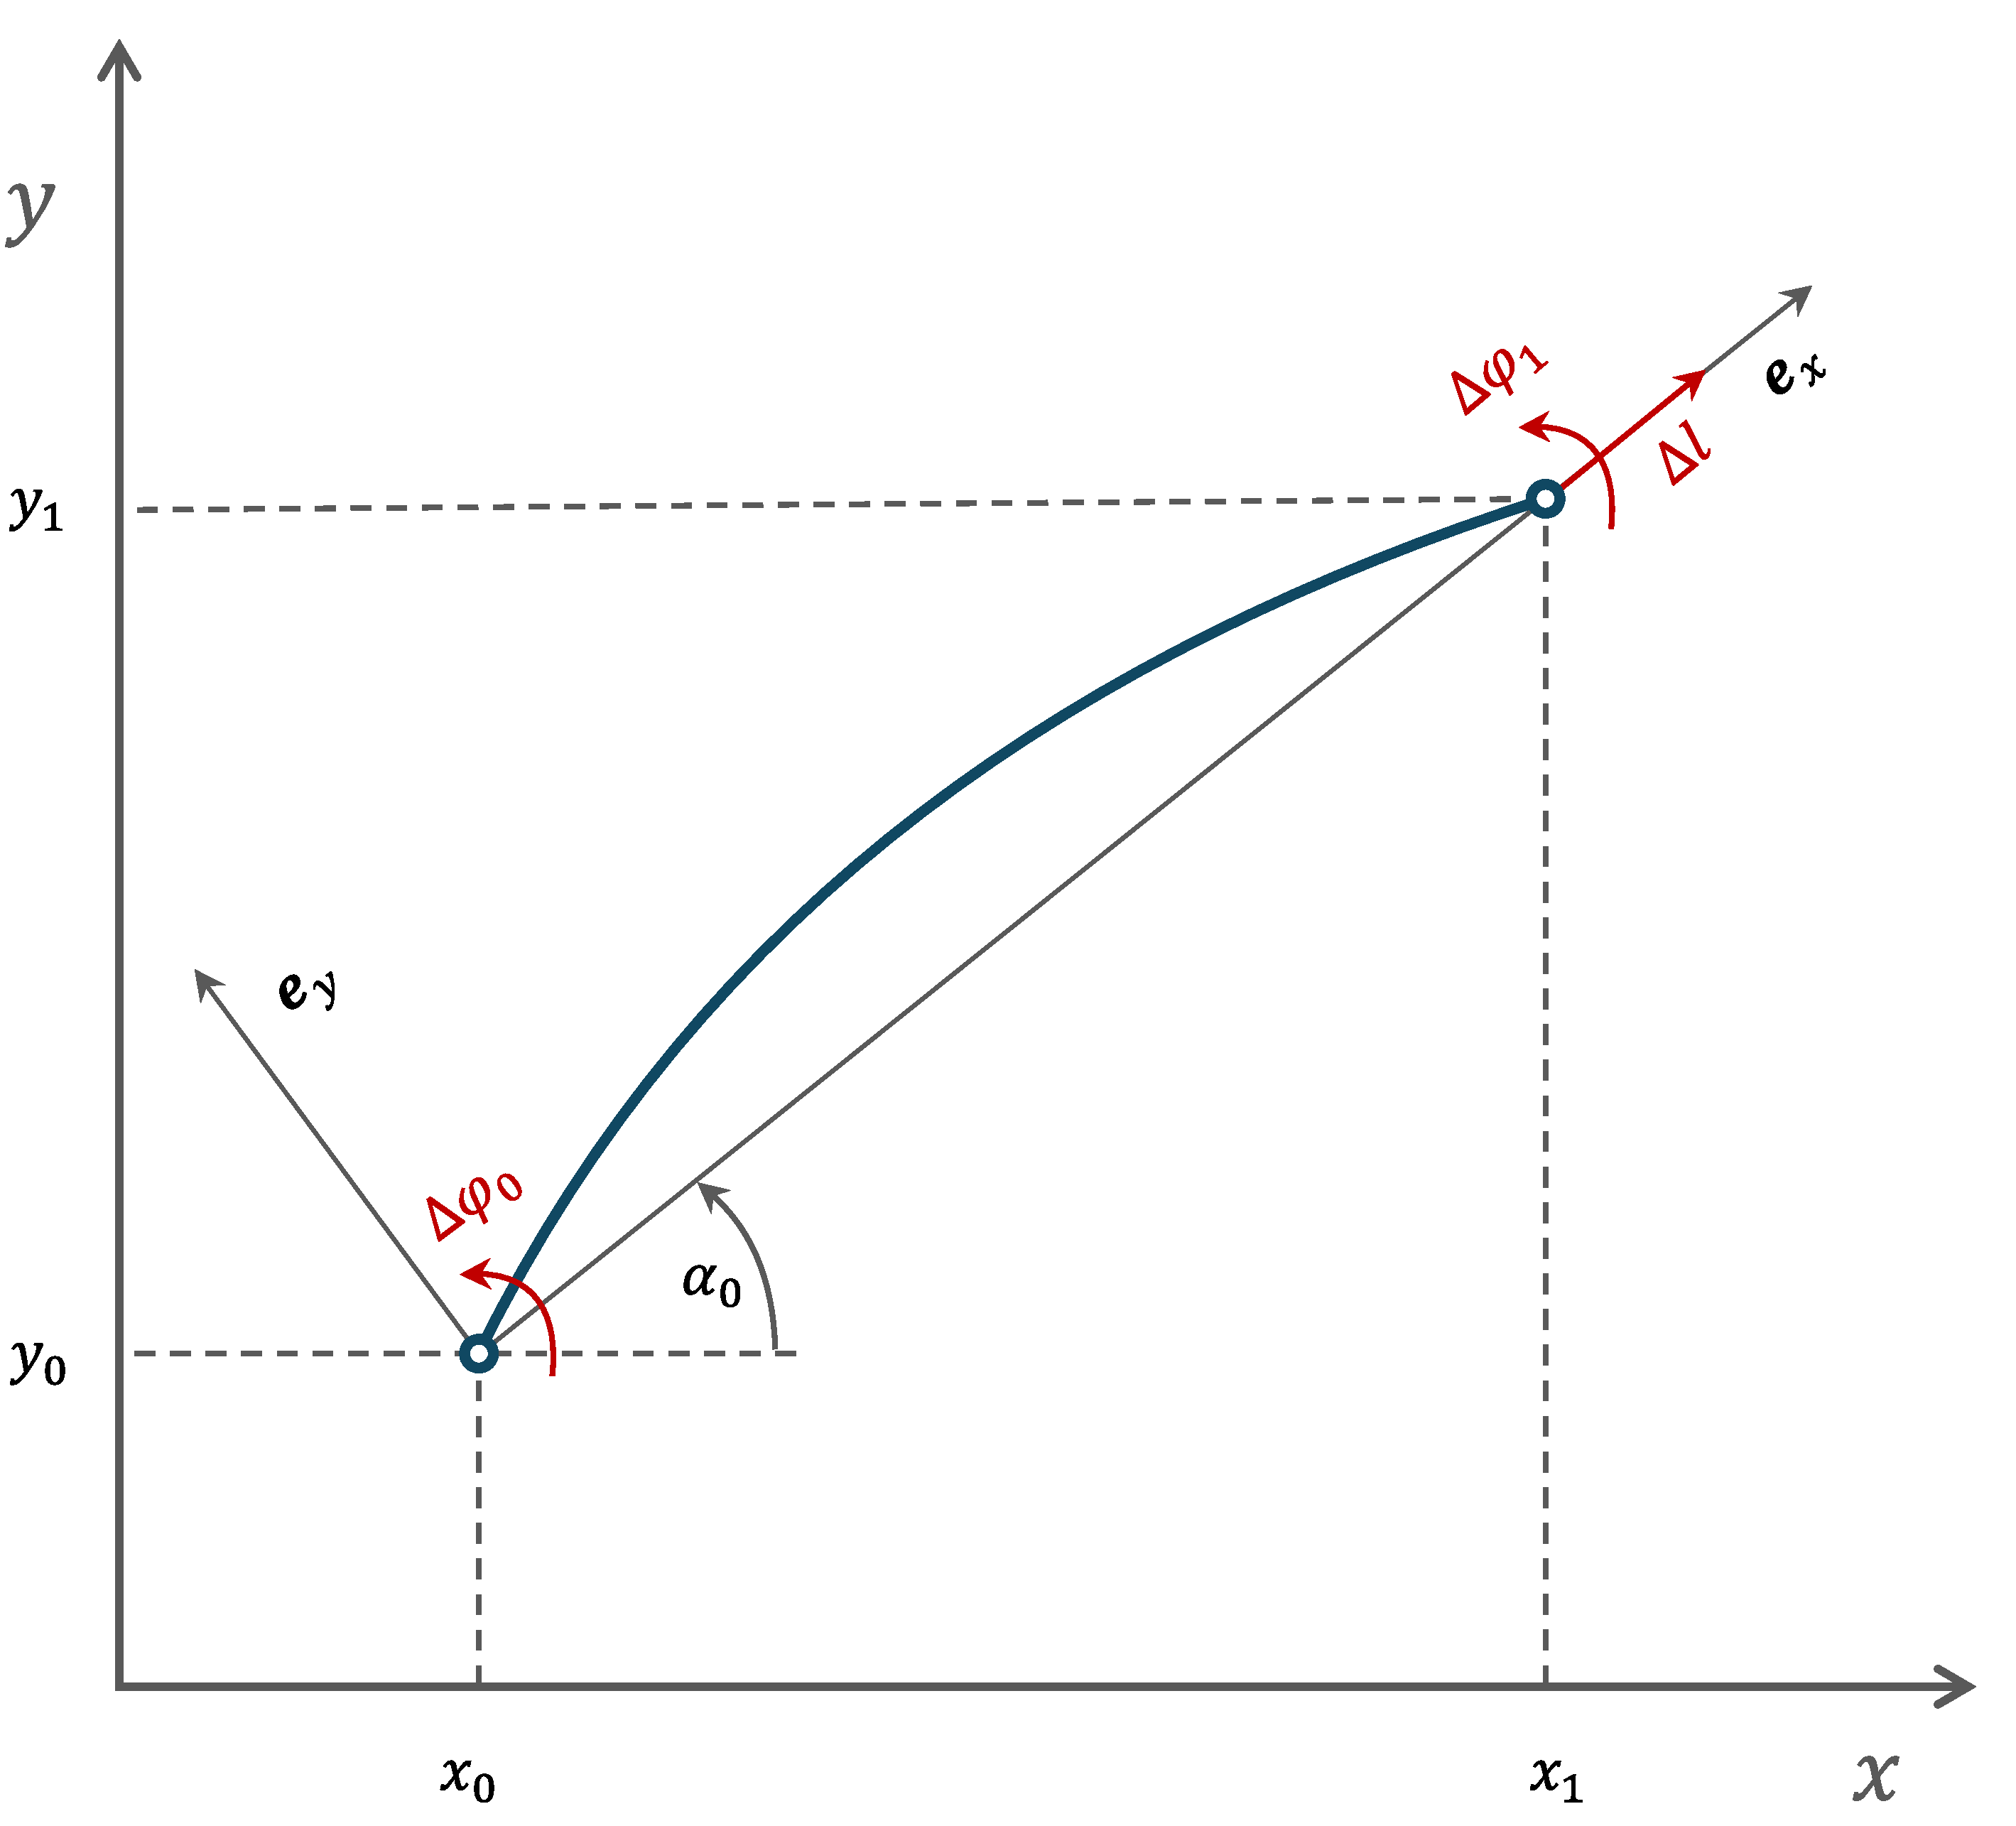
\includegraphics[width=0.5\textwidth]{figures/elements/beam-element-frame.pdf}
\caption{Local reference frame}
\label{fig:beam-element-frame}
\end{figure}

The x-axis can therefore be defined by the normalized direction vector

\begin{equation}
\boldsymbol{t} = \frac{\boldsymbol{r}_1 - \boldsymbol{r}_0}{\left|\boldsymbol{r}_1 - \boldsymbol{r}_0\right|}.
\end{equation}

To describe the elastic deformation of the element relative to this reference frame, three displacement coordinates are needed.
This is because the beam segment's position and rotation is now fixed with respect to the moving reference frame, taking away three of the original six degrees of freedom.
We choose the elastic displacements

\begin{equation}
\boldsymbol{u}_{e} = \begin{bmatrix}
\Delta l \\
\Delta \varphi_0 \\
\Delta \varphi_1 \\
\end{bmatrix}
\end{equation}

where $\Delta l$ is the elongation of the element along the local x-axis and $\Delta \varphi_0$, $\Delta \varphi_1$ are the changes in rotation angle at the two nodes.
The original displacements $\Delta\boldsymbol{u}$ of the beam segment can be expressed in terms of the new displacements as

\begin{equation}
\boldsymbol{u} =
\begin{bmatrix}
\Delta x_0 \\ \Delta y_0 \\ \Delta \varphi_0 \\ \Delta x_1 \\ \Delta y_1 \\ \Delta \varphi_1
\end{bmatrix}
=
\begin{bmatrix}
0 & 0 & 0 \\
0 & 0 & 0 \\
0 & 1 & 0 \\
t_x & 0 & 0 \\
t_y & 0 & 0 \\
0 & 0 & 1 \\
\end{bmatrix}
\begin{bmatrix}\Delta l \\ \Delta\varphi_0 \\ \Delta\varphi_1 \end{bmatrix}
=
\boldsymbol{T}\,\boldsymbol{u}_e.
\end{equation}

Therefore the stiffness matrix $\overline{\boldsymbol{K}}$ with respect to the local displacements is

% WxMaxima input:
%
%(%i4)	K: matrix(
%	 [k_00, k_01, k_02, k_03, k_04, k_05], 
%	 [k_10, k_11, k_12, k_13, k_14, k_15], 
%	 [k_20, k_21, k_22, k_23, k_24, k_25], 
%	 [k_30, k_31, k_32, k_33, k_34, k_35], 
%	 [k_40, k_41, k_42, k_43, k_44, k_45], 
%	 [k_50, k_51, k_52, k_53, k_54, k_55]
%	);
%
%(%i5)	T: matrix(
%	 [0,0,0], 
%	 [0,0,0], 
%	 [0,1,0], 
%	 [e_x,0,0], 
%	 [e_y,0,0], 
%	 [0,0,1]
%	);
%
%(%i6)	transpose(T).K.T;

\begin{align}
\overline{\boldsymbol{K}} &= \boldsymbol{T}^\intercal\boldsymbol{K}\boldsymbol{T} \notag \\
&=
\begin{bmatrix}
0 & 0 & 0 & t_x & t_y & 0 \\
0 & 0 & 1 & 0 & 0 & 0 \\
0 & 0 & 0 & 0 & 0 & 1 \\
\end{bmatrix}
\begin{bmatrix}
k_{00} & k_{01} & k_{02} & k_{03} & k_{04} & k_{05} \\
k_{10} & k_{11} & k_{12} & k_{13} & k_{14} & k_{15} \\
k_{20} & k_{21} & k_{22} & k_{23} & k_{24} & k_{25} \\
k_{30} & k_{31} & k_{32} & k_{33} & k_{34} & k_{35} \\
k_{40} & k_{41} & k_{42} & k_{43} & k_{44} & k_{45} \\
k_{50} & k_{51} & k_{52} & k_{53} & k_{54} & k_{55} \\
\end{bmatrix}
\begin{bmatrix}
0 & 0 & 0 \\
0 & 0 & 0 \\
0 & 1 & 0 \\
t_x & 0 & 0 \\
t_y & 0 & 0 \\
0 & 0 & 1 \\
\end{bmatrix} \notag \\
&=
\renewcommand\arraystretch{1.5}
\begin{bmatrix}
t_y \left(t_y k_{44} + t_x k_{43}\right) + t_x \left(t_y k_{34} + t_x k_{33}\right) & t_y k_{42} + t_x k_{32} & t_y k_{45} + t_x k_{35} \\
t_y k_{24} + t_x k_{23} & k_{22} & k_{25} \\
t_y k_{54} + t_x k_{53} & k_{52} & k_{55} \\
\end{bmatrix}
\end{align}

and the evaluation matrices for forces and strains, respectively, take the form
%
\begin{align}
\overline{\boldsymbol{E}} = \boldsymbol{E}\boldsymbol{T} &=
\begin{bmatrix}
e_{00} & e_{01} & e_{02} & e_{03} & e_{04} & e_{05} \\
e_{10} & e_{11} & e_{12} & e_{13} & e_{14} & e_{15} \\
e_{20} & e_{21} & e_{22} & e_{23} & e_{24} & e_{25} \\
\end{bmatrix}
\begin{bmatrix}
0 & 0 & 0 \\
0 & 0 & 0 \\
0 & 1 & 0 \\
t_x & 0 & 0 \\
t_y & 0 & 0 \\
0 & 0 & 1 \\
\end{bmatrix} \notag \\
&=
\begin{bmatrix}
t_x e_{03} + t_y e_{04} & e_{02} & e_{05} \\
t_x e_{13} + t_y e_{14} & e_{12} & e_{15} \\
t_x e_{23} + t_y e_{24} & e_{22} & e_{25} \\
\end{bmatrix}
\end{align}

\textcolor{red}{Remove detailed matrix expressions if not used in code}

\newpage
\subsection{Corotational Kinematics}

Express the elastic displacements in terms of the overall displacements as

\begin{equation}
\renewcommand\arraystretch{1.5}
\boldsymbol{u}_{e}(t) =
\begin{bmatrix}
\Delta l(t) \\
\Delta \varphi_0(t) \\
\Delta \varphi_1(t) \\ 
\end{bmatrix}
=
\begin{bmatrix}
l(t) - l(0) \\
\varphi_0(t) - \alpha(t) - \beta_0 \\
\varphi_1(t) - \alpha(t) - \beta_1 \\
\end{bmatrix}.
\end{equation}

Using
%
\begin{align}
\alpha(t) &= \mathrm{arctan2}\left(\Delta y,\,\Delta x\right) \\
l(t) &= \sqrt{\Delta x^2 + \Delta y^2}
\end{align}

and the two constant angular offsets
%
\begin{align}
\beta_0 &= \varphi_0(0) - \alpha(0), \\
\beta_1 &= \varphi_1(0) - \alpha(0).
\end{align}

There is one pitfall in these equations that needs to be addressed when implementing them.
Since the $\mathrm{arctan2}$ function is used for determining the orientation angle $\alpha(t)$ of the reference frame, the resulting value will be bound to the interval $[-\pi,\,\pi]$ and wrap around at $\alpha = \pm\pi$.
The nodal rotation angles $\varphi_0(t)$ and $\varphi_1(t)$ on the other hand are not bound to this interval because they don't wrap around.
When subtracting two such angles, as is done above, the resulting differences $\Delta \varphi_0(t)$ and $\Delta \varphi_1(t)$ can be off by multiples of $2\pi$ when one or more wrap-arounds have occurred.
This can easily be solved by normalizing $\Delta \varphi_0(t)$ and $\Delta \varphi_1(t)$ afterwards, which means adding or subtracting $2\pi$ until they lie in the interval $[-\pi,\,\pi]$.
The problem does not carry over to derivatives since the rate of change of the angles is not affected by added or subtracted constants.

Since the rigid body motion of the element does not produce any strain, the potential energy of the element is determined only by the elastic deformations and the corresponding stiffness matrix as

\begin{equation}
\Pi = \frac{1}{2}\boldsymbol{u}_{e}^\intercal\,\boldsymbol{K}_{e}\,\boldsymbol{u}_{e}.
\end{equation}

Therefore the nonlinear elastic forces of the element are

\begin{align}
\boldsymbol{Q}(\boldsymbol{q}) &= \frac{\partial\Pi}{\partial\boldsymbol{q}} = \frac{\partial\Pi}{\partial\boldsymbol{u}_e}\frac{\partial\boldsymbol{u}_e}{\partial\boldsymbol{q}} = \boldsymbol{J}^\intercal(\boldsymbol{q})\boldsymbol{K}_{e}\,\boldsymbol{u}_{e}
\end{align}

Derivatives:

\begin{equation}
\renewcommand\arraystretch{1.5}
\boldsymbol{J}(\boldsymbol{q}) =
\frac{\partial}{\partial\boldsymbol{q}}
\begin{bmatrix}
\Delta l \\
\Delta \varphi_0 \\
\Delta \varphi_1 \\
\end{bmatrix}
=
\begin{bmatrix}
-\frac{\Delta x}{l} & -\frac{\Delta y}{l} & 0 & \frac{\Delta x}{l} & \frac{\Delta y}{l} & 0 \\
-\frac{\Delta y}{l^2} & \frac{\Delta x}{l^2} & 1, & \frac{\Delta y}{l^2} & -\frac{\Delta x}{l^2} & 0 \\
-\frac{\Delta y}{l^2} & \frac{\Delta x}{l^2} & 0, & \frac{\Delta y}{l^2} & -\frac{\Delta x}{l^2} & 1 \\
\end{bmatrix}
\end{equation}

\newpage



\newpage
\subsection{Corotational Reference Frame}

In the previous section we found the stiffness matrix $\boldsymbol{K}_e$ of the beam segment, i.e. a description of its static behaviour for the small displacements

\begin{equation}
\boldsymbol{u}_e(t) = \begin{bmatrix}
\Delta l(t), & \Delta \varphi_0(t), & \Delta \varphi_1(t)
\end{bmatrix}^\intercal
\end{equation}

with respect to an attached reference frame.
Let's now consider the same beam segment under the potentially large nodal displacements

\begin{equation}
\boldsymbol{q}(t) = \begin{bmatrix}
x_{0}(t), & y_{0}(t), & \varphi_0(t), & x_{1}(t), & y_{1}(t), & \varphi_1(t)
\end{bmatrix}^\intercal.
\end{equation}

At this point the key assumption of the corotational formulation is introduced.
We assume that the overall displacements~$\boldsymbol{q}(t)$ are a superposition of a small elastic deformation~$\boldsymbol{u}_e(t)$ and a large rigid body motion (translation + rotation) that represents the geometrical nonlinearity of the element.

\begin{figure}[h]
\centering
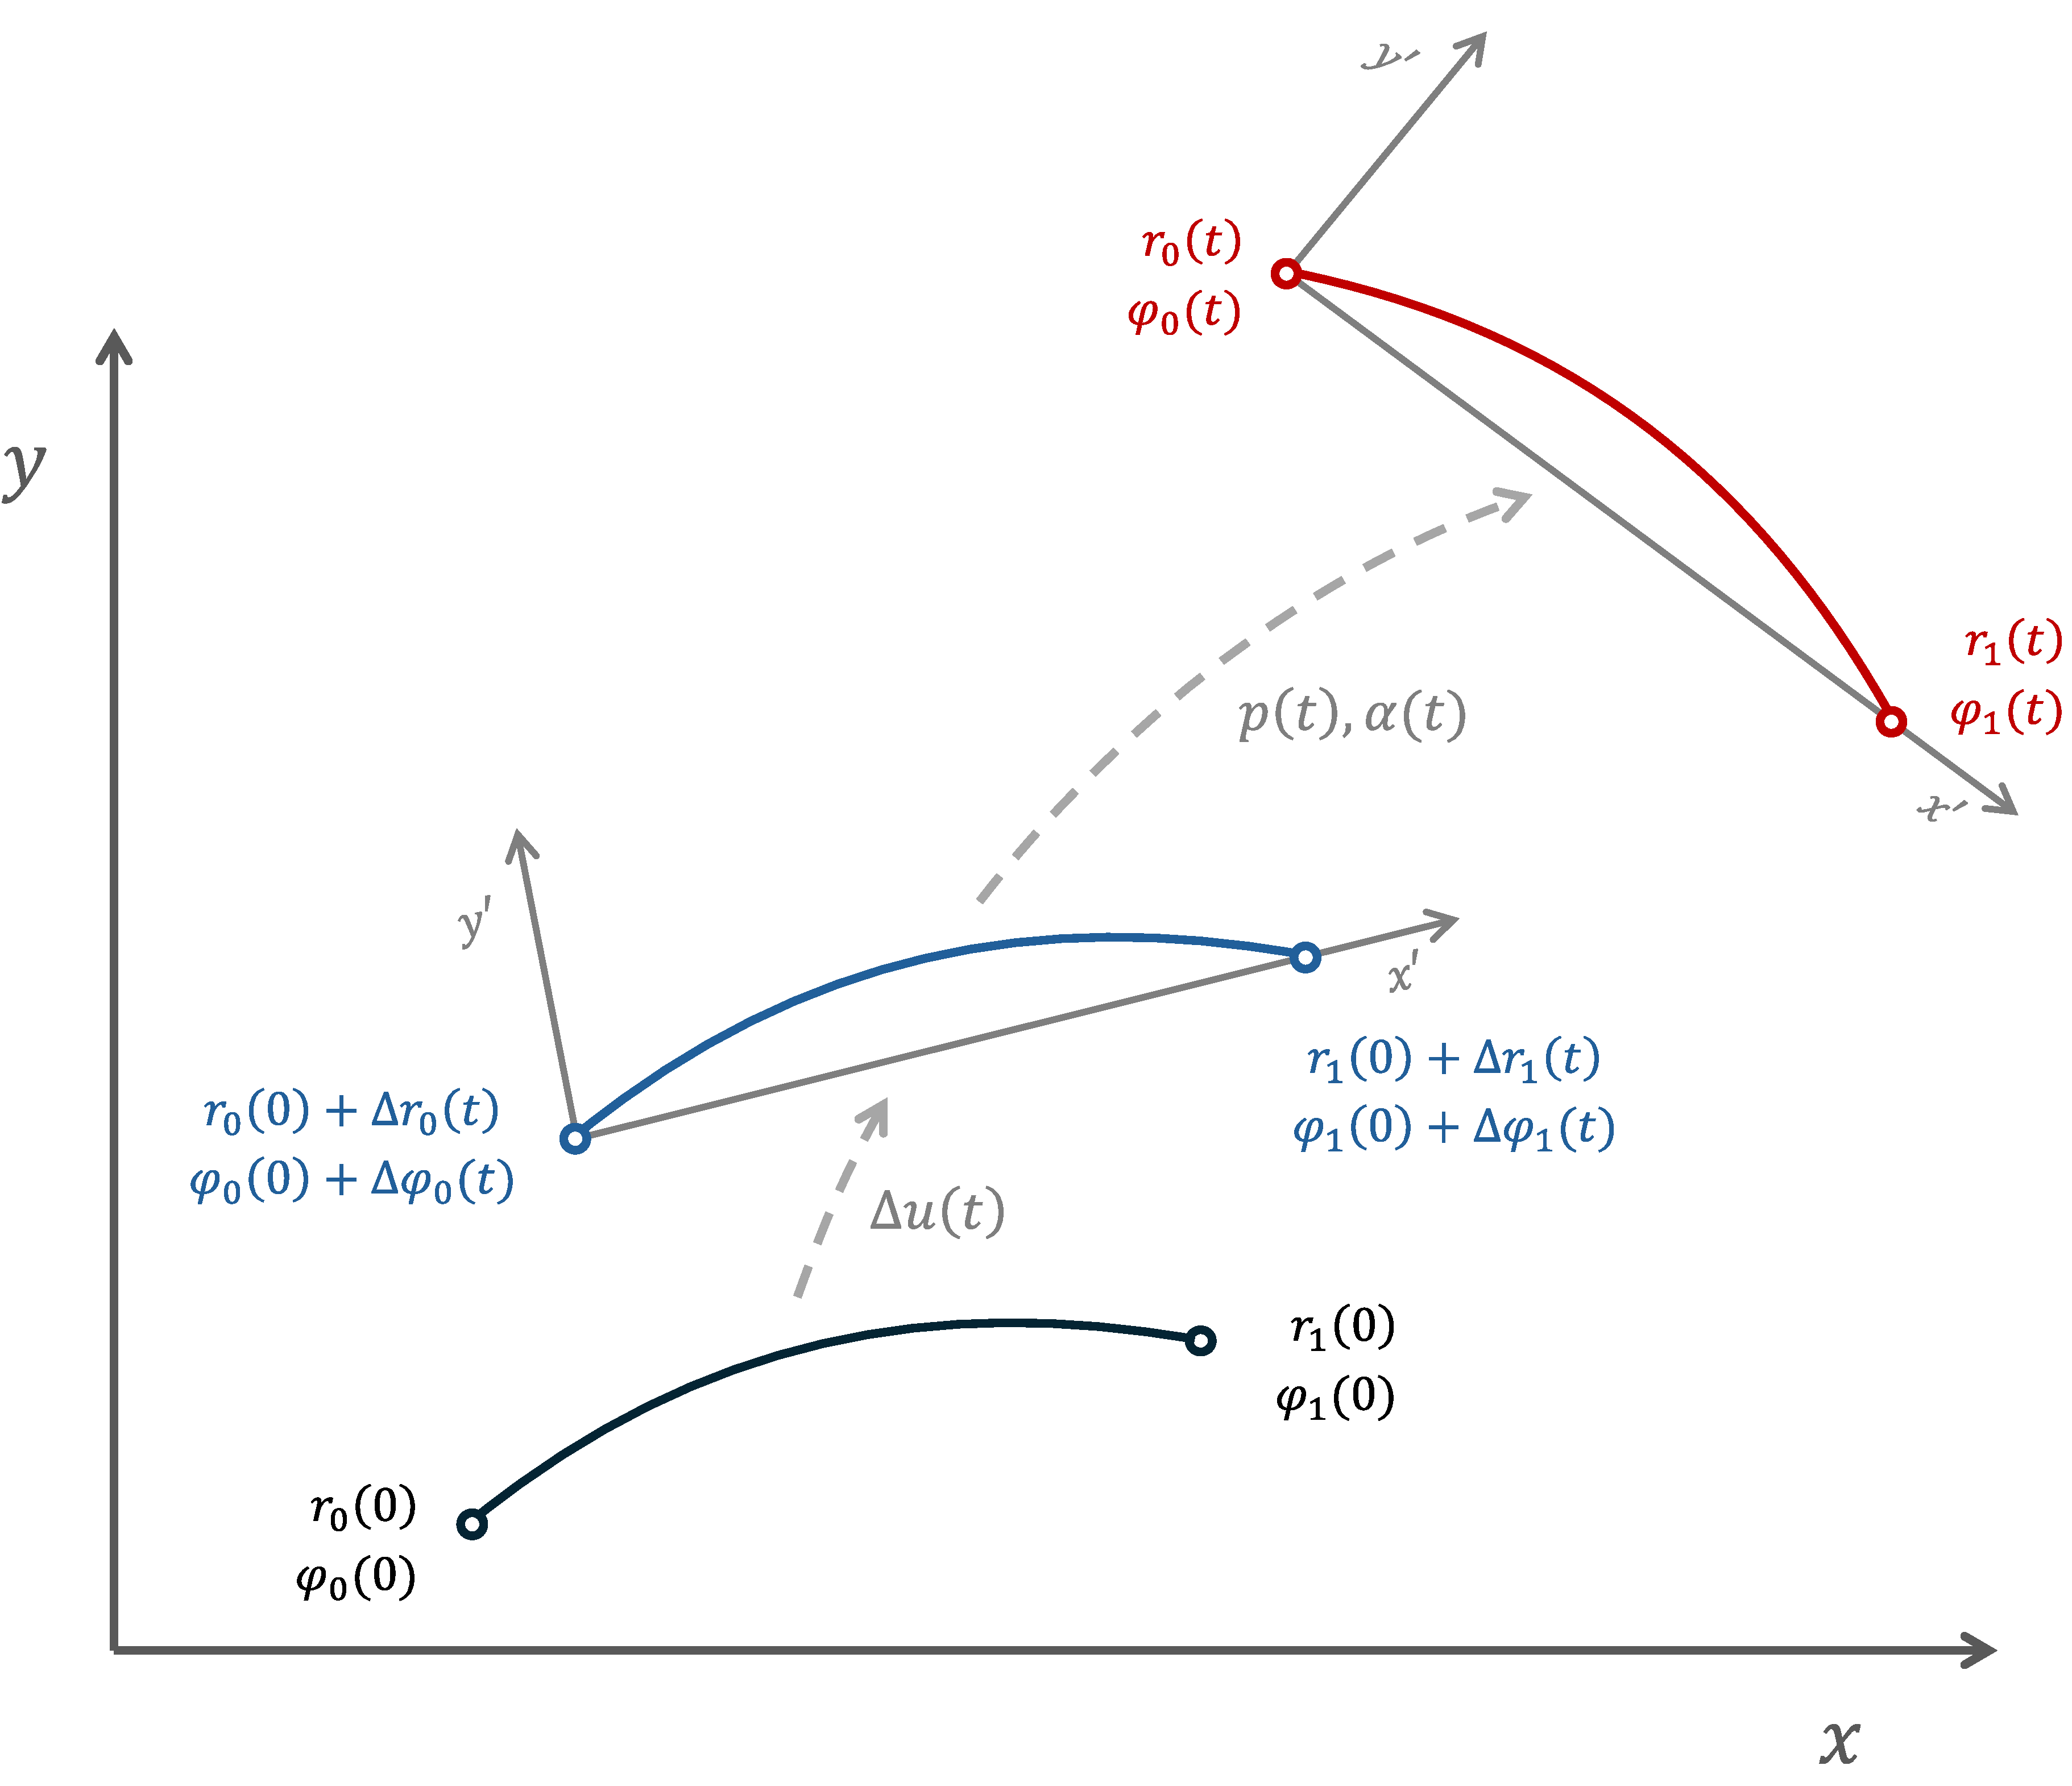
\includegraphics[width=0.8\textwidth]{figures/elements/beam-element-corotational.pdf}
\caption{Initial state (black), elastic deformation (blue) and rigid body motion (red) of the beam element}
\label{fig:beam-element-corotatrional}
\end{figure}

Extracting the rigid body motion by using a pinned reference frame:

\begin{align}
p(t) &= r_{0}(t) - r_{0}(0) - \Delta r_0(t) \\
\alpha(t) &= \angle\left(r_1(t) - r_0(t)\right) - \angle\left(r_1(0) + \Delta r_1(0) - r_0(0) - \Delta r_0(t)\right)
\end{align}

Kinematic relations:

\begin{align}
r_0(t) &= r_0(0) + \Delta r_0(t) + p(t) = r_0(t) \\
\varphi_0(t) &= \varphi_0(0) + \Delta\varphi_0(t) + \alpha(t) \\
\notag \\
r_1(t) &= r_0(t) + \lVert r_1(0) - r_0(0) + \Delta r_1(t) - \Delta r_0(t) \rVert\boldsymbol{e}_x(t) \\
\varphi_1(t) &= \varphi_1(0) + \Delta\varphi_1(t) + \alpha(t)
\end{align}

\newpage
\subsection{Mass Matrix}

As already mentioned previously \textcolor{red}{TODO: Mention}, mass matrices that are consistent with the corotational formulation tend to be fairly complicated.
For efficiency reasons, however, we would ideally want a mass matrix that is constant and diagonal, even if it's just an approximation.
That's why we derive the mass matrix in way that in't consisent with the way the elastic forces were derived, but leads to a result that has these properties.

Let's start with some general considerations before we introduce any approximations.
Let the function $\boldsymbol{p}(x,\,y,\,z)$ describt the position of the material point $(x,\,y,\,z)$ in the deformed state of the element in cartesian coordinates.
With the density $\rho$ that may vary over the element, we can express the virtual work of the inertia forces of the element as
%
\begin{align}
\delta W_{M} &= \int_{V} \delta\boldsymbol{p}^\intercal\rho\,\ddot{\boldsymbol{p}}\,dV = \int_{V} \rho\left(\frac{\partial\boldsymbol{p}}{\partial\boldsymbol{u}}\delta\boldsymbol{u}\right)^\intercal\left(\frac{\partial\boldsymbol{p}}{\partial\boldsymbol{u}}\ddot{\boldsymbol{u}}\right)\,dV = \delta\boldsymbol{u}^\intercal\underbrace{\left(\int_{V} \rho\,\frac{\partial\boldsymbol{p}}{\partial\boldsymbol{u}}^\intercal\frac{\partial\boldsymbol{p}}{\partial\boldsymbol{u}}\,dV\right)}_{\boldsymbol{M}}\ddot{\boldsymbol{u}}.
\end{align}

which gives us a general expression for the mass matrix.
In order to develop this further, we have to get more explicit about our position function.
For describing the deformation field of a beam, we write $\boldsymbol{p}$ as

\begin{equation}
\boldsymbol{p}(x,\,y,\,z) = \boldsymbol{r}(x) + y\,\boldsymbol{n}(x) + z\,\boldsymbol{b}(x)
\end{equation}

where $\boldsymbol{r}(x)$ is the beam's centerline, $\boldsymbol{n}(x)$ is the beam's normal vector and $\boldsymbol{b}(x)$ is the binormal vector (pointing out of the plane).
Further expansion and simplification of the mass matrix then leads to
%
\begin{align}
\boldsymbol{M} &= \int_{V} \rho\,\frac{\partial\boldsymbol{p}}{\partial\boldsymbol{u}}^\intercal\frac{\partial\boldsymbol{p}}{\partial\boldsymbol{u}}\,dV \notag \\
&= \int_{V} \rho\,\left(\frac{\partial\boldsymbol{r}}{\partial\boldsymbol{u}} + y\,\frac{\partial\boldsymbol{n}}{\partial\boldsymbol{u}}\right)^\intercal\left(\frac{\partial\boldsymbol{r}}{\partial\boldsymbol{u}} + y\,\frac{\partial\boldsymbol{n}}{\partial\boldsymbol{u}}\right)\,dV \notag \\
&= \int_{V} \left(\rho\,\frac{\partial\boldsymbol{r}}{\partial\boldsymbol{u}}^\intercal\frac{\partial\boldsymbol{r}}{\partial\boldsymbol{u}} + \rho y\,\frac{\partial\boldsymbol{n}}{\partial\boldsymbol{u}}^\intercal\frac{\partial\boldsymbol{r}}{\partial\boldsymbol{u}} + \rho y\,\frac{\partial\boldsymbol{r}}{\partial\boldsymbol{u}}^\intercal\frac{\partial\boldsymbol{n}}{\partial\boldsymbol{u}} + \rho y^2\,\frac{\partial\boldsymbol{n}}{\partial\boldsymbol{u}}^\intercal\frac{\partial\boldsymbol{n}}{\partial\boldsymbol{u}}\right)\,dV \notag \\
&= \int_{s_1}^{s_2} \left(\rho A\,\frac{\partial\boldsymbol{r}}{\partial\boldsymbol{u}}^\intercal\frac{\partial\boldsymbol{r}}{\partial\boldsymbol{u}} + \rho S\,\left(\frac{\partial\boldsymbol{n}}{\partial\boldsymbol{u}}^\intercal\frac{\partial\boldsymbol{r}}{\partial\boldsymbol{u}} + \frac{\partial\boldsymbol{r}}{\partial\boldsymbol{u}}^\intercal\frac{\partial\boldsymbol{n}}{\partial\boldsymbol{u}}\right) + \rho I\,\frac{\partial\boldsymbol{n}}{\partial\boldsymbol{u}}^\intercal\frac{\partial\boldsymbol{n}}{\partial\boldsymbol{u}}\right)\,ds
\end{align}

In the last step, the following three integrals over the beam's cross section have been introduced:
%
\begin{align}
\rho A(s) &= \int_A \rho\,dA \\
\rho S(s) &= \int_A \rho y\,dA \\
\rho I(s) &= \int_A \rho y^2\,dA
\end{align}

The first one, $\rho A$, is the linear density of the beam axis, i.e. the mass per unit length.
Mass matrix terms associated with this factor account for the overall motion of the beam axis.
The second one, $\rho S$, is the static moment of the cross section, weighted by its density, and is related to the excentricity of the center of gravity.
If the beam axis passed through the center of gravity of the cross sections, as is often assumed, this term would be zero.
Since we deliberately did not make this assumption, we will keep those terms for now.
The final one, $\rho I$ is the second moment of inertia of the section, weighted by its density, and accounts for the rotational inertia of the section itself.

\textcolor{red}{Introduce linear shape functions here}

The only thing left to do now is to express the derivatives $\nicefrac{\partial\boldsymbol{r}}{\partial\boldsymbol{u}}$ and $\nicefrac{\partial\boldsymbol{n}}{\partial\boldsymbol{u}}$ in terms of the shape function matrices $\boldsymbol{S}_x$, $\boldsymbol{S}_y$ and $\boldsymbol{S}_\varphi$.
This is straightforward and leads to

\begin{align}
\frac{\partial\boldsymbol{r}}{\partial\boldsymbol{u}}
&=
\frac{\partial}{\partial\boldsymbol{u}}
\begin{bmatrix}
\boldsymbol{S}_x^\intercal\boldsymbol{u} \\ \boldsymbol{S}_y^\intercal\boldsymbol{u}
\end{bmatrix}
=
\begin{bmatrix}
\boldsymbol{S}_x^\intercal \\ \boldsymbol{S}_y^\intercal
\end{bmatrix}
\\
\frac{\partial\boldsymbol{n}}{\partial\boldsymbol{u}}
&=
\frac{\partial}{\partial\boldsymbol{u}}
\begin{bmatrix}
\sin(\varphi) \\ \cos(\varphi)
\end{bmatrix}
=
\begin{bmatrix}
\boldsymbol{S}_\varphi^\intercal\cos(\varphi) \\ -\boldsymbol{S}_\varphi^\intercal\sin(\varphi)
\end{bmatrix}
\end{align}

Putting everything together, the mass matrix in its exact version becomes
%
\begin{equation}
\boldsymbol{M} = \int_{s_0}^{s_3} \left(\rho A\left(\boldsymbol{S}_x\boldsymbol{S}_x^\intercal + \boldsymbol{S}_y\boldsymbol{S}_y^\intercal\right) + \rho I\boldsymbol{S}_\varphi\boldsymbol{S}_\varphi^\intercal + \rho S\left(\left(\boldsymbol{S}_\varphi\boldsymbol{S}_x^\intercal + \boldsymbol{S}_x\boldsymbol{S}_\varphi^\intercal\right)\cos(\varphi) - \left(\boldsymbol{S}_\varphi\boldsymbol{S}_y^\intercal + \boldsymbol{S}_y\boldsymbol{S}_\varphi^\intercal\right)\sin(\varphi)\right)\right)\,ds
\end{equation}

In order to obtain a constant mass matrix, we neglect the influence of the coupling term associated with $\rho S$, leaving the simplified mass matrix

\begin{equation}
\boldsymbol{M} \approx \int_{s_0}^{s_1} \left(\rho A\left(\boldsymbol{S}_x\boldsymbol{S}_x^\intercal + \boldsymbol{S}_y\boldsymbol{S}_y^\intercal\right) + \rho I\boldsymbol{S}_\varphi\boldsymbol{S}_\varphi^\intercal\right)\,ds.
\end{equation}

This is justifiable because we are not really interested in the rotary motion of the cross sections.
We have to keep the term associated with $\rho I$ however, otherwise the mass matrix would become singular.

Diagonalized result when using the nodes as integration points (Newton-Cotes formula):

\begin{equation}
\boldsymbol{M} = \frac{s_1- s_0}{2}\begin{bmatrix}
\rho A(s_0) \\
& \rho A(s_0) \\
& & \rho I(s_0) \\
& & & \rho A(s_1) \\
& & & & \rho A(s_1) \\
& & & & & \rho I(s_1) \\
\end{bmatrix}
\end{equation}

Alternatively, the mass of the element can be computed exactly and distributed to the nodes such that the first node carries the mass of the first half of the element and the second node carries the second half.


\begin{align}
m_{0} &= \int_{s_0}^{s_m} \rho A(s)\,ds, \quad m_{1} = \int_{s_m}^{s_1} \rho A(s)\,ds \\
J_{0} &= \frac{1}{2}(s_1- s_0)\rho I(s_0), \quad J_{1} = \frac{1}{2}(s_1- s_0)\rho I(s_1)
\end{align}

\begin{equation}
\boldsymbol{M} = \begin{bmatrix}
m_0 \\
& m_0 \\
& & J_0 \\
& & & m_1 \\
& & & & m_1 \\
& & & & & J_1 \\
\end{bmatrix}
\end{equation}


\newpage
\section{Linear Curved Element}

\subsection*{Kinematics of Small Deformations}

Consider the beam segment shown in figure \ref{fig:linear-curved-beam-sections} whose undeformed shape is given by the reference curve $\boldsymbol{r}(s)$ and associated orientation angle $\varphi(s)$ in the direction of the reference curve.
The parameter $s$ is the arc length of the curve.

\begin{figure}[h]
\centering
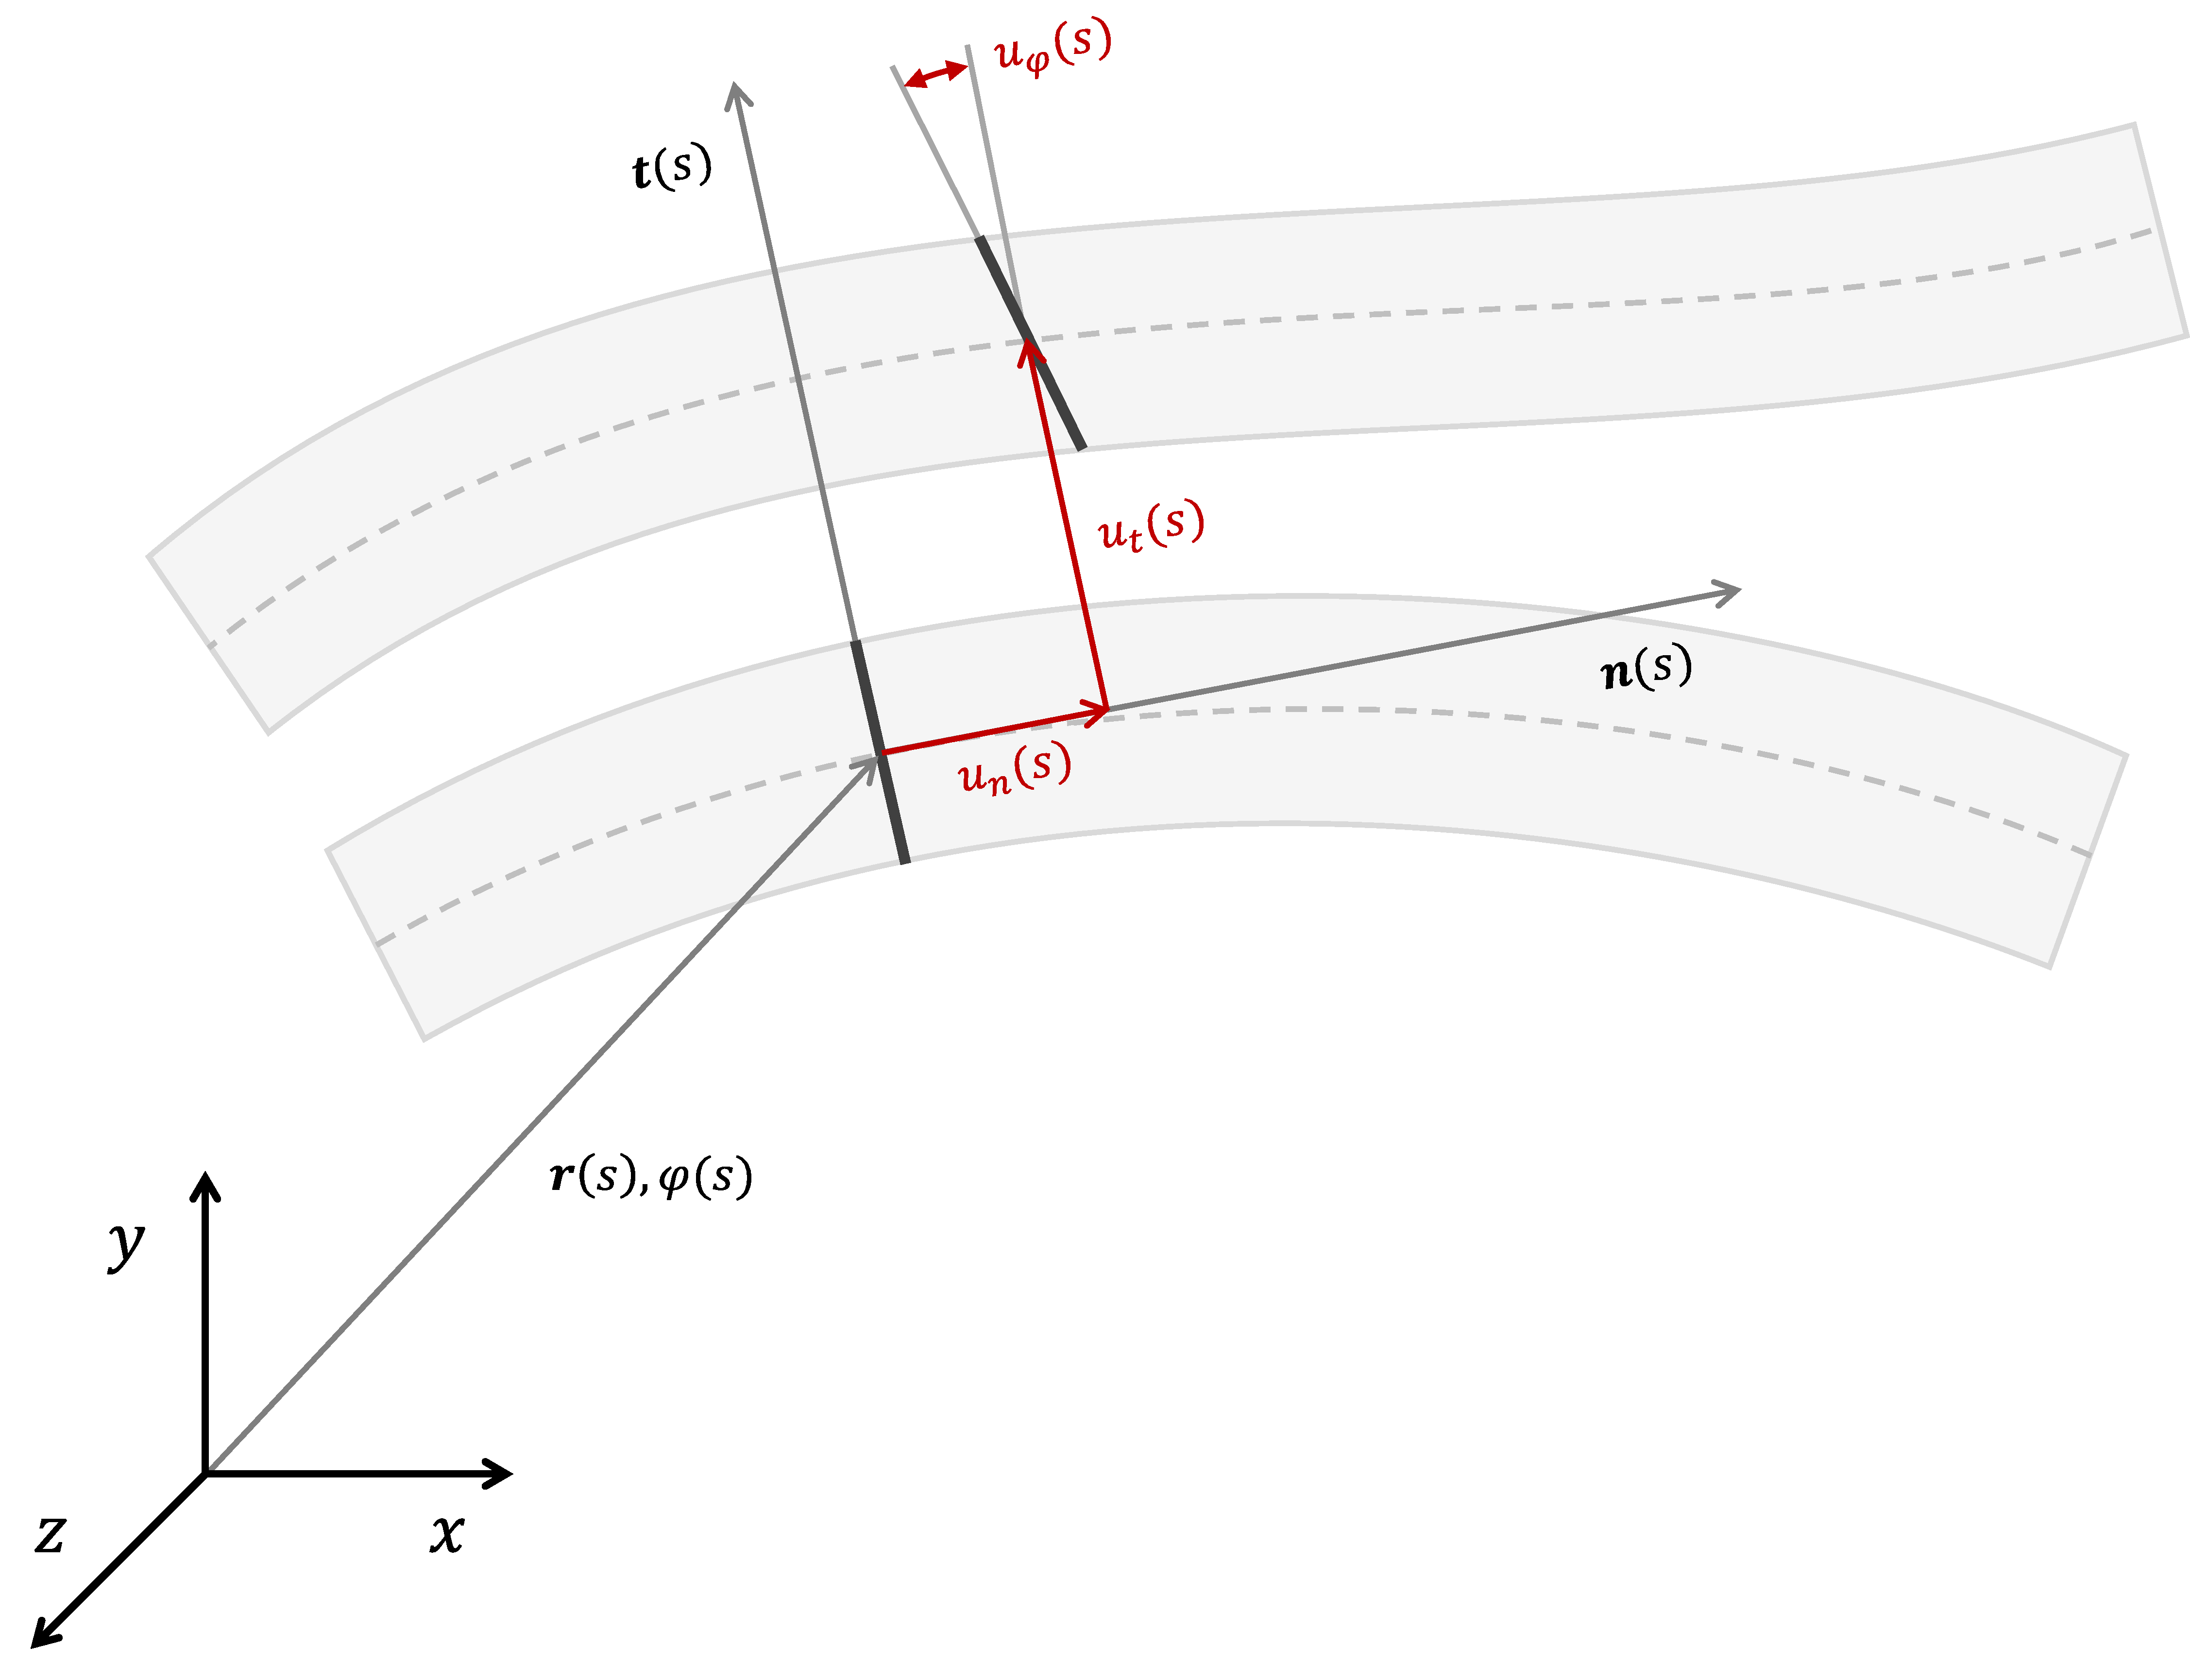
\includegraphics[width=0.8\textwidth]{figures/elements/linear-curved-beam-sections.pdf}
\caption{Curved beam segment with continuous displacement functions}
\label{fig:linear-curved-beam-sections}
\end{figure}

We describe the (small) deformation of this beam segment by the normal displacements $u_n(s)$ in the direction of the beam axis, the transversal displacements $u_t(s)$ and the rotational displacement $u_\varphi(s)$ of the cross sections.
These deformations are defined within the tangential reference frame $\boldsymbol{n}(s),\,\boldsymbol{t}(s)$ as shown the figure.

Within this tangent reference system we can obtain the displacement function $\boldsymbol{u}(x,y,z)$, i.e. a function that assigns each cartesian material point $x,\,y,\,z$ a displacement vector, as

\begin{align}
\boldsymbol{u}(x,y,z)
=
\begin{bmatrix}
u_n(x) - y\,u_\varphi(x) \\
u_t(x) + y \\
0
\end{bmatrix}
\end{align}

Here the small angle approximations $\sin(u_\varphi) \approx u_\varphi$ and $\cos(u_\varphi) \approx 1$ have been used.

Infinitesimal strains:

\begin{align}
\varepsilon_{xx} &= \frac{1}{2}\left(\frac{\partial u_x}{\partial x} + \frac{\partial u_x}{\partial x}\right) = u_n'(x) - y\,u_\varphi'(x) \\
\varepsilon_{xy} &= \frac{1}{2}\left(\frac{\partial u_x}{\partial y} + \frac{\partial u_y}{\partial x}\right) = \frac{1}{2}\left(u_t'(x) - u_\varphi(x)\right)
\end{align}

Generalized strains:

\begin{align}
\varepsilon &= u_n'(x) \\
\kappa &= u_\varphi'(x) \\
\gamma &= u_t'(x) - u_\varphi(x)
\end{align}

\newpage
\subsection*{Finite Element Discretization}

\begin{figure}[h]
\centering
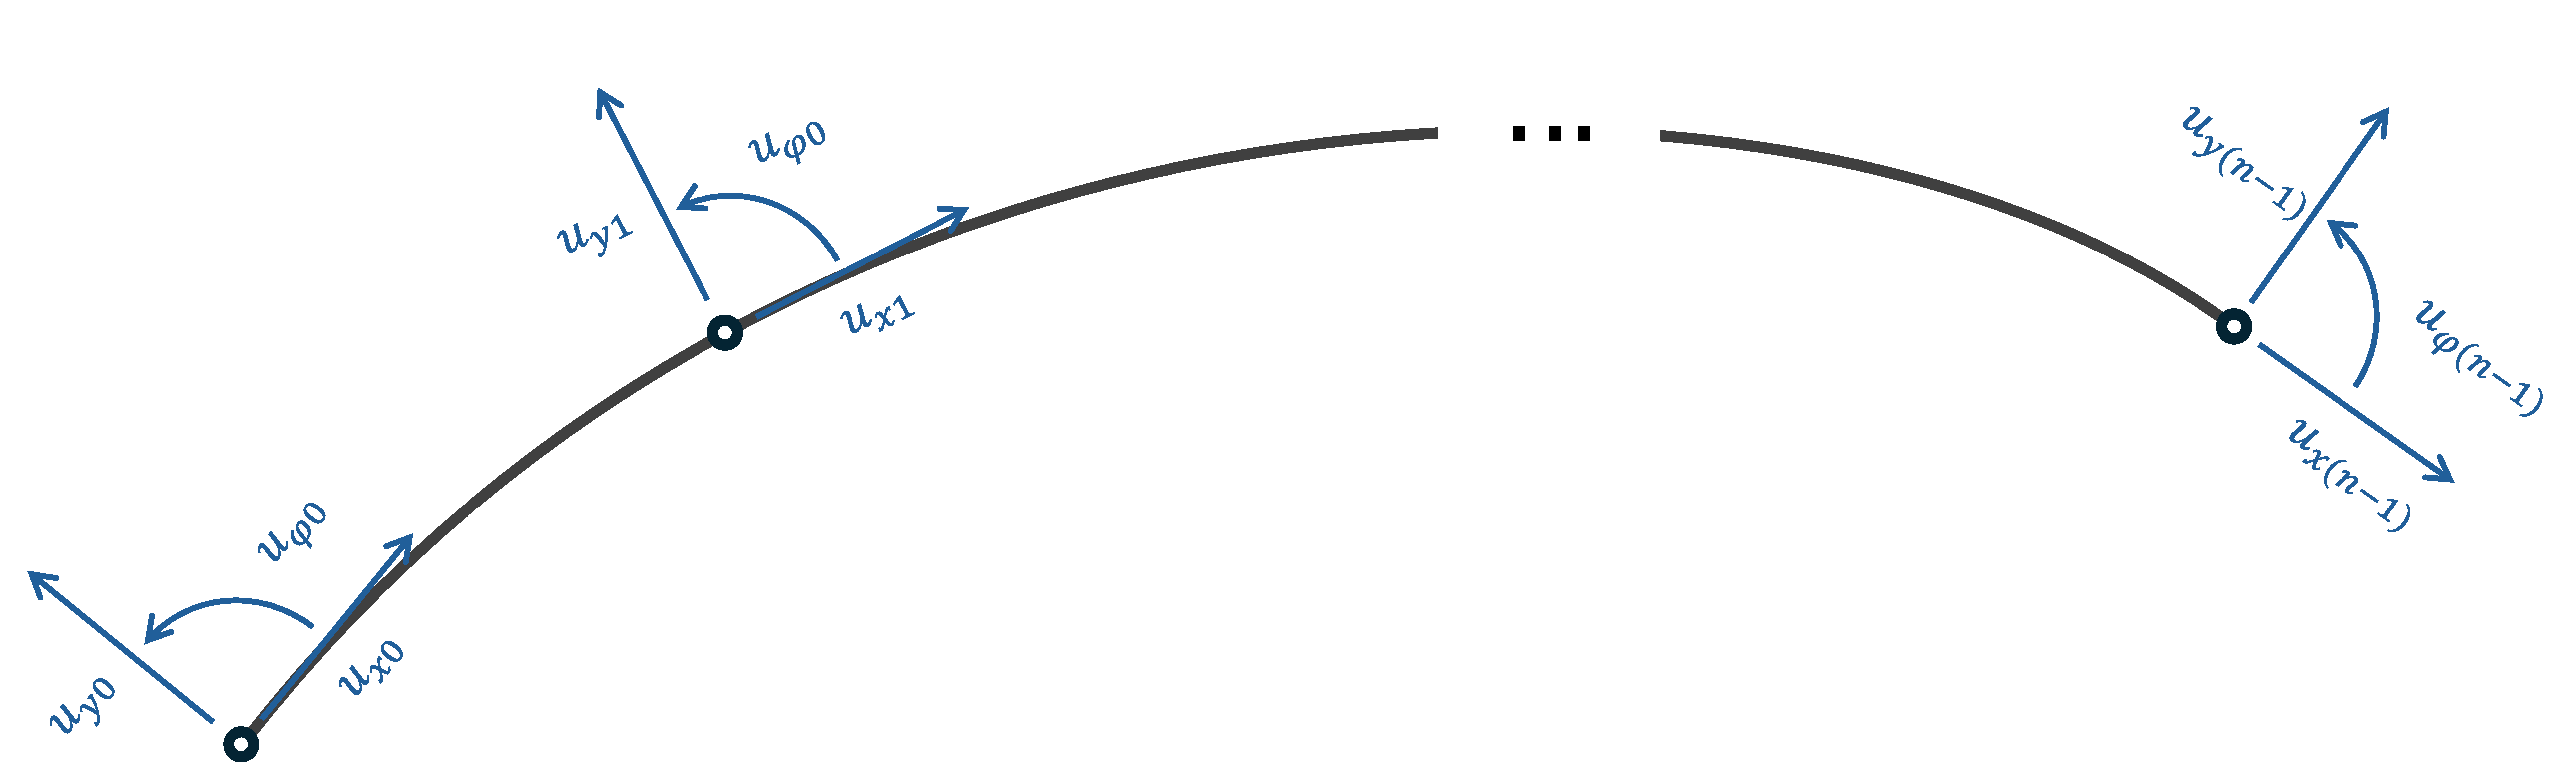
\includegraphics[width=0.8\textwidth]{figures/elements/linear-curved-beam-nodes.pdf}
\caption{Curved beam element with discrete nodes and displacements}
\label{fig:linear-curved-beam-nodes}
\end{figure}


Tangential, normal and rotational displacements:

\begin{align}
u_n(s) &= (1-\zeta) u_{n0} + \zeta u_{n1} = \boldsymbol{S}^\intercal_n(s) \boldsymbol{u} \\
u_t(s) &= (1-\zeta) u_{t0} + \zeta u_{t1} = \boldsymbol{S}^\intercal_t(s) \boldsymbol{u} \\
u_\varphi(s) &= (1-\zeta) u_{\varphi 0} + \zeta u_{\varphi 1} = \boldsymbol{S}^\intercal_\varphi(s) \boldsymbol{u}
\end{align}

Strain vector:

\begin{equation}
\underbrace{
\begin{bmatrix}
\varepsilon \\ \kappa \\ \gamma
\end{bmatrix}
}_{\boldsymbol{e}}
=
\underbrace{
\begin{bmatrix}
\boldsymbol{S}'^\intercal_n \\ \boldsymbol{S}'^\intercal_\varphi \\ \boldsymbol{S}'^\intercal_t - \boldsymbol{S}^\intercal_\varphi
\end{bmatrix}
}_{\boldsymbol{S}_e}
\boldsymbol{u}
\end{equation}

\begin{equation}
\boldsymbol{S}_e = \begin{bmatrix}
1-\zeta & 0 & 0 & \zeta & 0 & 0 \\
0 & 1-\zeta & 0 & 0 & \zeta & 0 \\
0 & 0 & 1-\zeta & 0 & 0 & \zeta \\
\end{bmatrix}
\end{equation}


Potential energy:

\begin{align}
\Pi = \frac{1}{2}\int_{s_0}^{s_1} \boldsymbol{e}^\intercal\boldsymbol{f}\,ds = \frac{1}{2}\int_{s_0}^{s_1} \boldsymbol{e}^\intercal\boldsymbol{C}\boldsymbol{e}\,ds = 
\end{align}



\newpage
\section{Beam Element (GEBF)}

Describe the beam's kinematics with the position $\boldsymbol{r}(x)$ of the beam axis and the angle $\varphi(x)$ of the cross sections.
The tangent, normal- and binormal vectors are

\begin{equation}
\boldsymbol{t}(x) = \begin{bmatrix}
\phantom{-}\cos(\varphi) \\ -\sin(\varphi) \\ 0
\end{bmatrix}, \quad
\boldsymbol{n}(x) = \begin{bmatrix}
\sin(\varphi) \\ \cos(\varphi) \\ 0
\end{bmatrix}, \quad
\boldsymbol{b}(x) = \begin{bmatrix}
0 \\ 0 \\ 1
\end{bmatrix}, \quad
\end{equation}

which can be combined into the rotation matrix $\boldsymbol{R} = \left[\boldsymbol{t},\,\boldsymbol{n},\,\boldsymbol{b}\right]$.
The deformed position of the point $(x,\,y\,z)$ in reference coordinates is found to be

\begin{equation}
\boldsymbol{p}(x,y,z) = \boldsymbol{r}(x) + y\,\boldsymbol{n}(x) + z\,\boldsymbol{b}(x).
\end{equation}

Therefore the deformation gradient is

\begin{equation}
\boldsymbol{F}
=
\begin{bmatrix}
\frac{\partial\boldsymbol{p}}{\partial x}, & \frac{\partial\boldsymbol{p}}{\partial y}, & \frac{\partial\boldsymbol{p}}{\partial z} 
\end{bmatrix}
=
\begin{bmatrix}
r_x' - y\varphi'\cos(\varphi) & \sin(\varphi) & 0\\
r_y' - y\varphi'\sin(\varphi) & \cos(\varphi) & 0\\
0                             & 0             & 1
\end{bmatrix}
\end{equation}

By writing the deformation gradient as $\boldsymbol{F} = \boldsymbol{R}\tilde{\boldsymbol{F}}$ we can decompose it into the rotation $\boldsymbol{R}$ of the cross section and the deformation $\tilde{\boldsymbol{F}}$ with respect to the rotated section.
Since the rotation matrix $\boldsymbol{R}$ is orthonormal, we can compute $\tilde{\boldsymbol{F}}$ as

\begin{equation}
\tilde{\boldsymbol{F}} = \boldsymbol{R}^\intercal\boldsymbol{F} =
\begin{bmatrix}
r_x'\cos(\varphi) + r_y'\sin(\varphi) - y\varphi' & 0 & 0 \\
r_y'\cos(\varphi) - r_x'\sin(\varphi) & 1 & 0 \\
0 & 0 & 1
\end{bmatrix}
\end{equation}

Finally we assume the deformation $\tilde{\boldsymbol{F}}$ to be small and compute the corresponding infinitesimal strain tensor as,

\begin{equation}
\boldsymbol{E} = \frac{1}{2}\left(\tilde{\boldsymbol{F}} + \tilde{\boldsymbol{F}}^\intercal\right) - \boldsymbol{I} =
\begin{bmatrix}
r_x'\cos(\varphi) + r_y'\sin(\varphi) - y\varphi' - 1 & \frac{1}{2}\left(r_y'\cos(\varphi) - r_x'\sin(\varphi)\right) & 0 \\
\frac{1}{2}\left(r_y'\cos(\varphi) - r_x'\sin(\varphi)\right) & 0 & 0 \\
0 & 0 & 0
\end{bmatrix}
\end{equation}

Since the strain tensor is symmetric, there are only two independent and non-vanishing strain components, the axial strain $\varepsilon_{xx}$ and the shear strain $\varepsilon_{xy}$.
Using the shear angle $\gamma_{xy} = 2\varepsilon_{xy}$ instead, we can write them as

\begin{align}
\varepsilon_{xx} &= \varepsilon - y\kappa \\
\gamma_{xy} &= \gamma
\end{align}

With the axial strain $\varepsilon$ and curvature $\kappa$ of the beam axis and the shear angle $\gamma$ that define the generalized strain vector

\begin{equation}
\boldsymbol{\varepsilon}
=
\begin{bmatrix}
\varepsilon \\ \gamma \\ \kappa
\end{bmatrix}
=
\begin{bmatrix}
r_x'\cos(\varphi) + r_y'\sin(\varphi) - 1 \\
r_y'\cos(\varphi) - r_x'\sin(\varphi) \\
\varphi'
\end{bmatrix}
\end{equation}

\begin{align}
\varepsilon &= r_x'\cos(\varphi) + r_y'\sin(\varphi) - 1 \\
\gamma &= r_y'\cos(\varphi) - r_x'\sin(\varphi) \\
\kappa &= \varphi'
\end{align}

\subsection*{Internal Forces}

Starting from the virtual work of internal forces, with the linear elastic material reltionship $\sigma_{xx} = E\varepsilon{xx}$ and $\tau_{xy} = E\gamma{xx}$

\begin{align}
\delta W_{I} &= \int_{V} \delta\boldsymbol{\varepsilon}^\intercal\boldsymbol{\sigma}\,dV = \int_{V}\left(\delta\varepsilon_{xx}\sigma_{xx} + \delta\gamma_{xy}\tau_{xy}\right)\,dV = \int_{V}\left(E\delta\varepsilon_{xx}\varepsilon_{xx} + G\delta\gamma_{xy}\gamma_{xy}\right)\,dV \notag \\
&= \int_{V}\left(E\delta\left(\varepsilon - y\kappa\right)\left(\varepsilon - y\kappa\right) + G\delta\gamma\gamma \right)\,dV \notag \\
&= \int_{V}\left( \left(E\varepsilon - Ey\kappa\right)\delta\varepsilon + \left(Ey^2\kappa - Ey\varepsilon\right)\delta\kappa + G\gamma\delta\gamma \right)\,dV \notag \\
&= \int_{s_1}^{s_2}\left( \left(C_{\varepsilon\varepsilon}\varepsilon + C_{\varepsilon\kappa}\kappa\right)\delta\varepsilon + \left(C_{\kappa\kappa}\kappa + C_{\varepsilon\kappa}\varepsilon\right)\delta\kappa + C_{\gamma\gamma}\gamma\delta\gamma \right)\,ds \\
&= \int_{s_1}^{s_2}\left( N\delta\varepsilon + M\delta\kappa + Q\delta\gamma \right)\,ds
\end{align}

With the cross section integrals

\begin{equation}
C_{\varepsilon\varepsilon} = \int_{A} E\,dA, \quad C_{\varepsilon\kappa} = -\int_{A} Ey\,dA, \quad C_{\kappa\kappa} = \int_{A} Ey^2\,dA, \quad C_{\gamma\gamma} = \int_{A} G\,dA
\end{equation}

Expressing the normal force $N$, the bending moment $M$ and the shear force $Q$ on the section:

\begin{align}
N &= \int_{A} \sigma_{xx}\,dA = \int_{A} E(\varepsilon - y\kappa)\,dA = C_{\varepsilon\varepsilon}\varepsilon + C_{\varepsilon\kappa}\kappa \\
M &= -\int_{A} y\sigma_{xx}\,dA = \int_{A} E(y^2\kappa - y\varepsilon)\,dA = C_{\kappa\kappa}\kappa + C_{\varepsilon\kappa}\varepsilon \\
Q &= \int_{A} \tau_{xy}\,dA = \int_{A} G\gamma\,dA = C_{\gamma\gamma}\gamma
\end{align}

So the $C$ constants are basically stiffness coefficinents between the generalized strains and the generalized forces on the cross section.
The relation can be expressed in matrix form as

\begin{equation}
\begin{bmatrix}
N \\ M \\ Q
\end{bmatrix}
=
\begin{bmatrix}
C_{\varepsilon\varepsilon} & C_{\varepsilon\kappa} & 0 \\
C_{\varepsilon\kappa} & C_{\varepsilon\varepsilon} & 0 \\
0 & 0 & C_{\gamma\gamma}
\end{bmatrix}
\begin{bmatrix}
\varepsilon \\ \kappa \\ \gamma
\end{bmatrix}
\end{equation}

\subsection{Quadratic shape functions (3 nodes)}

Source: https://numerichouse.wordpress.com/fembarsf/

Nodes at $\zeta = 0$, $\zeta = \frac{1}{2}$ and $\zeta = 1$ for the natural coordinate $\zeta(x) = \frac{x - s_{1}}{s_{2} - s_{1}}$

\begin{align}
S_1(x) &= -\frac{1}{2}\zeta + \frac{1}{2}\zeta^2 \\
S_2(x) &= 1 - \zeta^2 \\
S_3(x) &= \frac{1}{2}\zeta + \frac{1}{2}\zeta^2
\end{align}

Interpolation:

\begin{align}
r_x(x) &= S_1(x)\,x_1 + S_2(x)\,x_2 + S_3(x)\,x_3 = \boldsymbol{S}_{x}(x)^\intercal\boldsymbol{u} \\
r_y(x) &= S_1(x)\,y_1 + S_2(x)\,y_2 + S_3(x)\,y_3 = \boldsymbol{S}_{y}(x)^\intercal\boldsymbol{u} \\
\varphi(x) &= S_1(x)\,\varphi_1 + S_2(x)\,\varphi_2 + S_3(x)\,\varphi_3 = \boldsymbol{S}_{\varphi}(x)^\intercal\boldsymbol{u}
\end{align}

with the vector of nodal coordinates $\boldsymbol{u} = \left[x_1,\,y_1,\,\varphi_1,\,x_2,\,y_2,\,\varphi_2,\,x_3,\,y_3,\,\varphi_3\right]^\intercal$ and the shape matrices

\begin{align}
\boldsymbol{S}_{x}(x) &= \left[S_1,\,0,\,0,\,S_2,\,0,\,0,\,S_3,\,0,\,0\right]^\intercal \\
\boldsymbol{S}_{y}(x) &= \left[0,\,S_1,\,0,\,0,\,S_2,\,0,\,0,\,S_3,\,0\right]^\intercal \\
\boldsymbol{S}_{\varphi}(x) &= \left[0,\,0,\,S_1,\,0,\,0,\,S_2,\,0,\,0,\,S_3\right]^\intercal \\
\end{align}


\subsection{Cubic shape functions (4 nodes)}

Source: Lagrange interpolation, https://mathworld.wolfram.com/LagrangeInterpolatingPolynomial.html
Lagrange polynomials

\begin{equation}
S_{i}(s) = \prod_{k=0,\,k\neq i}^{n-1} \frac{s - s_k}{s_i - s_k}
\end{equation}

For $n=4$ this evaluates to the functiona
%
\begin{align}
S_0(s) &= \frac{s - s_1}{s_0 - s_1}\frac{s - s_2}{s_0 - s_2}\frac{s - s_3}{s_0 - s_3}, & S_1(s) &= \frac{s - s_0}{s_1 - s_0}\frac{s - s_2}{s_1 - s_2}\frac{s - s_3}{s_1 - s_3}, \notag \\
\notag \\
S_2(s) &= \frac{s - s_0}{s_2 - s_0}\frac{s - s_1}{s_2 - s_1}\frac{s - s_3}{s_2 - s_3}, & S_3(s) &= \frac{s - s_0}{s_3 - s_0}\frac{s - s_1}{s_3 - s_1}\frac{s - s_2}{s_3 - s_2}.
\end{align}

The position of the centerline as well as the rotation angle are interpolated by the same shape functions:

\begin{align}
r_x(x) &= \sum_{i=1}^4 S_{i}(\zeta)\,x_i = \boldsymbol{S}_{x}(x)^\intercal\boldsymbol{u} \\
r_y(x) &= \sum_{i=1}^4 S_{i}(\zeta)\,y_i = \boldsymbol{S}_{y}(x)^\intercal\boldsymbol{u} \\
\varphi(x) &= \sum_{i=1}^4 S_{i}(\zeta)\,\varphi_i = \boldsymbol{S}_{\varphi}(x)^\intercal\boldsymbol{u}
\end{align}

with the vector of nodal coordinates $\boldsymbol{u} = \left[x_1,\,y_1,\,\varphi_1,\,x_2,\,y_2,\,\varphi_2,\,x_3,\,y_3,\,\varphi_3,\,x_4,\,y_4,\,\varphi_4\right]^\intercal$ and the shape function matrices
%
\begin{align}
\boldsymbol{S}_{x}(x) &= \left[S_0,\,0,\,0,\,S_1,\,0,\,0,\,S_2,\,0,\,0,\,S_3,\,0,\,0\right]^\intercal \\
\boldsymbol{S}_{y}(x) &= \left[0,\,S_0,\,0,\,0,\,S_1,\,0,\,0,\,S_2,\,0,\,0,\,S_3,\,0\right]^\intercal \\
\boldsymbol{S}_{\varphi}(x) &= \left[0,\,0,\,S_0,\,0,\,0,\,S_1,\,0,\,0,\,S_2,\,0,\,0,\,S_3\right]^\intercal
\end{align}

\subsection{Internal forces}

Internal forces:
%
\begin{align}
\boldsymbol{Q}(\boldsymbol{u}) &= \int_{s_1}^{s_2}\left( \left(C_{\varepsilon\varepsilon}\varepsilon + C_{\varepsilon\kappa}\kappa\right)\frac{\partial\varepsilon}{\partial\boldsymbol{u}} + \left(C_{\kappa\kappa}\kappa + C_{\varepsilon\kappa}\varepsilon\right)\frac{\partial\kappa}{\partial\boldsymbol{u}} + C_{\gamma\gamma}\gamma\frac{\partial\gamma}{\partial\boldsymbol{u}} \right)\,ds \\
&= \int_{s_1}^{s_2}\left( N\frac{\partial\varepsilon}{\partial\boldsymbol{u}} + M\frac{\partial\kappa}{\partial\boldsymbol{u}} + Q\frac{\partial\gamma}{\partial\boldsymbol{u}} \right)\,ds
\end{align}

Tangent stiffness matrix:
%
\begin{align}
\boldsymbol{K}(\boldsymbol{u}) &= \int_{s_1}^{s_2}\left( N\frac{\partial^2\varepsilon}{\partial\boldsymbol{u}^2} + M\frac{\partial^2\kappa}{\partial\boldsymbol{u}^2} + Q\frac{\partial^2\gamma}{\partial\boldsymbol{u}^2} + \frac{\partial N}{\partial\boldsymbol{u}}\frac{\partial\varepsilon}{\partial\boldsymbol{u}}^\intercal + \frac{\partial M}{\partial\boldsymbol{u}}\frac{\partial\kappa}{\partial\boldsymbol{u}}^\intercal + \frac{\partial Q}{\partial\boldsymbol{u}}\frac{\partial\gamma}{\partial\boldsymbol{u}}^\intercal \right)\,ds \\
\frac{\partial N}{\partial\boldsymbol{u}} &= C_{\varepsilon\varepsilon}\frac{\partial\varepsilon}{\partial\boldsymbol{u}} + C_{\varepsilon\kappa}\frac{\partial\kappa}{\partial\boldsymbol{u}}, \\
\notag \\
\frac{\partial M}{\partial\boldsymbol{u}} &= C_{\kappa\kappa}\frac{\partial\kappa}{\partial\boldsymbol{u}} + C_{\varepsilon\kappa}\frac{\partial\varepsilon}{\partial\boldsymbol{u}}, \\
\notag \\
\frac{\partial Q}{\partial\boldsymbol{u}} &= C_{\gamma\gamma}\frac{\partial\gamma}{\partial\boldsymbol{u}}
\end{align}

Partial derivatives of the strain components with respect to the coordinates:
%
\begin{align}
\frac{\partial\varepsilon}{\partial\boldsymbol{u}} &= \frac{\partial r_x'}{\partial\boldsymbol{u}}\cos(\varphi) + \frac{\partial r_y'}{\partial\boldsymbol{u}}\sin(\varphi) - r_x' \frac{\partial\varphi}{\partial\boldsymbol{u}}\sin(\varphi) + r_y' \frac{\partial\varphi}{\partial\boldsymbol{u}}\cos(\varphi) \notag \\
&= \boldsymbol{S}_x'\cos(\varphi) + \boldsymbol{S}_y'\sin(\varphi) + \boldsymbol{S}_\varphi\gamma \\
\notag \\
\frac{\partial\gamma}{\partial\boldsymbol{u}} &= \frac{\partial r_y'}{\partial\boldsymbol{u}}\cos(\varphi) - \frac{\partial r_x'}{\partial\boldsymbol{u}}\sin(\varphi) - r_y' \frac{\partial\varphi}{\partial\boldsymbol{u}}\sin(\varphi) - r_x' \frac{\partial\varphi}{\partial\boldsymbol{u}}\cos(\varphi) \notag \\
&= \boldsymbol{S}_y'\cos(\varphi) - \boldsymbol{S}_x'\sin(\varphi) - \boldsymbol{S}_\varphi(\varepsilon - 1) \\
\notag \\
\frac{\partial\kappa}{\partial\boldsymbol{u}} &= \boldsymbol{S}_\varphi'
\end{align}

And the second derivatives
%
\begin{align}
\frac{\partial^2\varepsilon}{\partial\boldsymbol{u}^2} &= \left(\boldsymbol{S}_y'\cos(\varphi) - \boldsymbol{S}_x'\sin(\varphi)\right)\boldsymbol{S}_\varphi^\intercal + \boldsymbol{S}_\varphi\frac{\partial\gamma}{\partial\boldsymbol{u}}^\intercal \\
\notag \\
\frac{\partial^2\gamma}{\partial\boldsymbol{u}^2} &= -\left(\boldsymbol{S}_y'\sin(\varphi) + \boldsymbol{S}_x'\cos(\varphi)\right)\boldsymbol{S}_\varphi^\intercal + \boldsymbol{S}_\varphi\frac{\partial\epsilon}{\partial\boldsymbol{u}}^\intercal \\
\notag \\
\frac{\partial^2\kappa}{\partial\boldsymbol{u}^2} &= \boldsymbol{0}
\end{align}

\subsection{Mass matrix}

Now we're going to look at the inertia forces and identify the element's mass matrix,
%
\begin{align}
\delta W_{M} &= \int_{V} \delta\boldsymbol{p}^\intercal\rho\,\ddot{\boldsymbol{p}}\,dV = \int_{V} \rho\left(\frac{\partial\boldsymbol{p}}{\partial\boldsymbol{u}}\delta\boldsymbol{u}\right)^\intercal\left(\frac{\partial\boldsymbol{p}}{\partial\boldsymbol{u}}\ddot{\boldsymbol{u}}\right)\,dV = \delta\boldsymbol{u}^\intercal\underbrace{\left(\int_{V} \rho\,\frac{\partial\boldsymbol{p}}{\partial\boldsymbol{u}}^\intercal\frac{\partial\boldsymbol{p}}{\partial\boldsymbol{u}}\,dV\right)}_{\boldsymbol{M}}\ddot{\boldsymbol{u}}.
\end{align}

Further expansion and simplification of the mass matrix leads to
%
\begin{align}
\boldsymbol{M} &= \int_{V} \rho\,\frac{\partial\boldsymbol{p}}{\partial\boldsymbol{u}}^\intercal\frac{\partial\boldsymbol{p}}{\partial\boldsymbol{u}}\,dV \notag \\
&= \int_{V} \rho\,\left(\frac{\partial\boldsymbol{r}}{\partial\boldsymbol{u}} + y\,\frac{\partial\boldsymbol{n}}{\partial\boldsymbol{u}}\right)^\intercal\left(\frac{\partial\boldsymbol{r}}{\partial\boldsymbol{u}} + y\,\frac{\partial\boldsymbol{n}}{\partial\boldsymbol{u}}\right)\,dV \notag \\
&= \int_{V} \left(\rho\,\frac{\partial\boldsymbol{r}}{\partial\boldsymbol{u}}^\intercal\frac{\partial\boldsymbol{r}}{\partial\boldsymbol{u}} + \rho y\,\frac{\partial\boldsymbol{n}}{\partial\boldsymbol{u}}^\intercal\frac{\partial\boldsymbol{r}}{\partial\boldsymbol{u}} + \rho y\,\frac{\partial\boldsymbol{r}}{\partial\boldsymbol{u}}^\intercal\frac{\partial\boldsymbol{n}}{\partial\boldsymbol{u}} + \rho y^2\,\frac{\partial\boldsymbol{n}}{\partial\boldsymbol{u}}^\intercal\frac{\partial\boldsymbol{n}}{\partial\boldsymbol{u}}\right)\,dV \notag \\
&= \int_{s_1}^{s_2} \left(\rho A\,\frac{\partial\boldsymbol{r}}{\partial\boldsymbol{u}}^\intercal\frac{\partial\boldsymbol{r}}{\partial\boldsymbol{u}} + \rho S\,\left(\frac{\partial\boldsymbol{n}}{\partial\boldsymbol{u}}^\intercal\frac{\partial\boldsymbol{r}}{\partial\boldsymbol{u}} + \frac{\partial\boldsymbol{r}}{\partial\boldsymbol{u}}^\intercal\frac{\partial\boldsymbol{n}}{\partial\boldsymbol{u}}\right) + \rho I\,\frac{\partial\boldsymbol{n}}{\partial\boldsymbol{u}}^\intercal\frac{\partial\boldsymbol{n}}{\partial\boldsymbol{u}}\right)\,ds
\end{align}

In the last step, the following three integrals over the beam's cross section have been factored out:
%
\begin{align}
\rho A(s) &= \int_A \rho\,dA \\
\rho S(s) &= \int_A \rho y\,dA \\
\rho I(s) &= \int_A \rho y^2\,dA
\end{align}

The first one, $\rho A$, is the linear density of the beam axis, i.e. the mass per unit length.
Mass matrix terms associated with this factor account for the overall motion of the beam axis.
The second one, $\rho S$, is the static moment of the cross section, weighted by its density, and is related to the excentricity of its center of gravity.
If the beam axis passed through the center of gravity of the cross sections, as is often assumed, this term would be zero.
Since we deliberately did not make this assumption, we will keep those terms.
The final one, $\rho I$ is the second moment of inertia of the section, weighted by its density, and accounts for the rotational inertia of the section itself.

The only thing left to do now is to express the derivatives $\nicefrac{\partial\boldsymbol{r}}{\partial\boldsymbol{u}}$ and $\nicefrac{\partial\boldsymbol{n}}{\partial\boldsymbol{u}}$ in terms of the shape function matrices $\boldsymbol{S}_x$, $\boldsymbol{S}_y$ and $\boldsymbol{S}_\varphi$.
This is straightforward and leads to

\begin{align}
\frac{\partial\boldsymbol{r}}{\partial\boldsymbol{u}}
&=
\frac{\partial}{\partial\boldsymbol{u}}
\begin{bmatrix}
\boldsymbol{S}_x^\intercal\boldsymbol{u} \\ \boldsymbol{S}_y^\intercal\boldsymbol{u}
\end{bmatrix}
=
\begin{bmatrix}
\boldsymbol{S}_x^\intercal \\ \boldsymbol{S}_y^\intercal
\end{bmatrix}
\\
\frac{\partial\boldsymbol{n}}{\partial\boldsymbol{u}}
&=
\frac{\partial}{\partial\boldsymbol{u}}
\begin{bmatrix}
\sin(\varphi) \\ \cos(\varphi)
\end{bmatrix}
=
\begin{bmatrix}
\boldsymbol{S}_\varphi^\intercal\cos(\varphi) \\ -\boldsymbol{S}_\varphi^\intercal\sin(\varphi)
\end{bmatrix}
\end{align}

Putting everything together, the mass matrix in its exact version becomes
%
\begin{equation}
\boldsymbol{M} = \int_{s_0}^{s_3} \left(\rho A\left(\boldsymbol{S}_x\boldsymbol{S}_x^\intercal + \boldsymbol{S}_y\boldsymbol{S}_y^\intercal\right) + \rho I\boldsymbol{S}_\varphi\boldsymbol{S}_\varphi^\intercal + \rho S\left(\left(\boldsymbol{S}_\varphi\boldsymbol{S}_x^\intercal + \boldsymbol{S}_x\boldsymbol{S}_\varphi^\intercal\right)\cos(\varphi) - \left(\boldsymbol{S}_\varphi\boldsymbol{S}_y^\intercal + \boldsymbol{S}_y\boldsymbol{S}_\varphi^\intercal\right)\sin(\varphi)\right)\right)\,ds
\end{equation}

In order to obtain a constant mass matrix, we neglect the influence of the coupling term associated with $\rho S$, leaving the simplified mass matrix

\begin{equation}
\boldsymbol{M} \approx \int_{s_0}^{s_3} \left(\rho A\left(\boldsymbol{S}_x\boldsymbol{S}_x^\intercal + \boldsymbol{S}_y\boldsymbol{S}_y^\intercal\right) + \rho I\boldsymbol{S}_\varphi\boldsymbol{S}_\varphi^\intercal\right)\,ds.
\end{equation}

This is justifiable because we are not really interested in the rotary motion of the cross sections.
We have to keep the term associated with $\rho I$ however, otherwise the mass matrix would become singular.

\subsection{Numerical Integration}

The expressions for the internal forces as well as the mass- and stiffness matrices each contain an integral over the length of the element.
Solving those integrals analytically can't be done without specifying how the cross section properties vary over the length of the element and even then it might not be possible.
Instead we use numerical integration to efficiently compute an approximation.
The class of integration schemes we are interested in approximates the integral as a weighted sum of function evaluations at various points in the interval,

\begin{equation}
\int_{a}^{b}f(x)\,dx \approx \sum_{i=0}^{n-1} w_{i}\,f(x_{i})
\end{equation}

where the $n$ points $x_{i}$ are the integration points and $w_{i}$ are the corresponding weights.
Such schemes are often called \textit{quadrature rules} and a key difference between many of them is the choice of integration points.
In the case of equidistant integration points we get the so called \textit{Newton-Cotes formulas}, which exist in an \textit{open} and \textit{closed} variant, depending on whether the integral boundaries $a$ and $b$ are to be evaluated or not.
A Newton-Cotes formula of order $n$ integrates a polynomial of degree $n$ exactly, which means that the method is accurate if the function $f(x)$ is well-approximated by a polynomial of order $n$ in the interval $[a,\,b]$.

A more accurate method is \textit{Gauss-Legendre quadrature}, where the integration points are not equally spaced but instead chosen in a way that maximizes accuracy.
The integration points do not contain the interval boundaries in this method.
Gauss-Legendre integration of order $n$ is exact for polynomials of degree $2n-1$, which is much better than the Newton-Cotes formulas.

Another method called \textit{Gauss-Lobatto quadrature} is very similar to Gauss-Legendre but does contain the interval boundaries as the integration points, which can be a practical advantage.
In return it is however not quite as accurate since it only integrates polynomials of degree $2n-3$ exactly.


Table \textcolor{red}{TODO} shows some of the points and weights for these three methods.
To put the properties of these methods into perspective, if we were to integrate a function that can be approximated by a polynomial of degree 5, we would need 5 integration points with the Newton-Cotes formula, 4 integration points with the Gauss-Lobatto formula and only 3 integration points with the Gauss-Legendre formula.
This is the reason why Gauss-Legendre is basically the standard integration method in finite element analysis.
One drawback from a practical perspective however is that the integration points are not equally spaced and don't generally coincide with the nodes of the element.
This is important because the integration points are the points where stresses, strains and other quantities of interest are evaluated.
Some possible ways to deal with this are listed below

\begin{enumerate}
\item Place the four nodes of the beam element equally spaced and use Newton-Cotes integration where the integration points are now equal to the element's nodes. This has the advantage that all quantities are evaluated at the element nodes. The obvious disadvantage is the poor accuracy of the method.
\item Place the four nodes equally spaced and use Gauss-Legendre quadrature where the integration points are distinct from the nodes. This is numerically efficient and accurate, but extra computation is required to obtain stresses and strains at the element's nodes.
\item Place the four nodes at the Gauss-Lobatto integration points and use that scheme for integration \textcolor{red}{TODO: Reference to spectral element method}. This leads to acceptable accuracy and efficient evaluation of results at the element nodes. The disadvantage is reduced control over the placement of the nodes.
\end{enumerate}

For this beam element we use method 2 for integration of the elastic forces and the tangent stiffness matrix.
The mass matrix however is integrated by method 1, because using the nodes of the element as the integration points leads to a diagonal/lumped approximation of the mass matrix as we will see in the following.

\newpage
\subsection{Diagonal Mass Matrix}

We can observe that the shape function terms $\boldsymbol{S}_x\boldsymbol{S}_x^\intercal$, $\boldsymbol{S}_y\boldsymbol{S}_y^\intercal$ and $\boldsymbol{S}_\varphi\boldsymbol{S}_\varphi^\intercal$ that make up the integrad of the mass matrix become diagonal at the nodal points $s_{0},\,\ldots,\,s_{3}$ of the element.
More specifically,

\begin{align}
\boldsymbol{S}_x(s_i)\boldsymbol{S}_x(s_i)^\intercal &= \mathrm{diag}(\boldsymbol{e}_{3i}) \\
\boldsymbol{S}_y(s_i)\boldsymbol{S}_y(s_i)^\intercal &= \mathrm{diag}(\boldsymbol{e}_{3i+1}) \\
\boldsymbol{S}_\varphi(s_i)\boldsymbol{S}_\varphi(s_i)^\intercal &= \mathrm{diag}(\boldsymbol{e}_{3i+2})
\end{align}

where $\boldsymbol{e}_{i}$ is the $i$-th unit vector.
This means that if we approximate the integral for the mass matrix by only sampling the integrand at the nodal points of the element, the resulting mass matrix is going to be diagonal, which is a very desirable property.
The cost for this is the reduced accuracy from using the Newton-Cotes formula instead of Gaussian quadrature.
Higher accuracy could have been obtained by using the Gauss-Lobatto method on suitably spaced nodes but introducing other practical disadvantages.

Since the accuracy of the mass matrix is not as critical for our application as for example the elastic forces, we carry out the integration \textcolor{red}{TODO: Eq-Refs} symbolically to obtain the following diagonal approximation for the mass matrix,

\begin{align}
\boldsymbol{M} &= \int_{s_0}^{s_3} \left(\rho A \boldsymbol{S}_x\boldsymbol{S}_x^\intercal + \rho A \boldsymbol{S}_y\boldsymbol{S}_y^\intercal + \rho I\boldsymbol{S}_\varphi\boldsymbol{S}_\varphi^\intercal\right)\,ds \notag \\
&\approx \sum_{s_i}w_i\left(\rho A(s_i)\boldsymbol{S}_x\boldsymbol{S}_x^\intercal(s_i) + \rho A(s_i)\boldsymbol{S}_y\boldsymbol{S}_y^\intercal(s_i) + \rho I(s_i)\boldsymbol{S}_\varphi\boldsymbol{S}_\varphi^\intercal(s_i)\right) \notag \\
&\approx  \sum_{s_i}w_i\left(\rho A(s_i)\,\mathrm{diag}(\boldsymbol{e}_{3i}) + \rho A(s_i)\,\mathrm{diag}(\boldsymbol{e}_{3i+1}) + \rho I(s_i)\,\mathrm{diag}(\boldsymbol{e}_{3i+2})\right) \notag \\
&\approx  \mathrm{diag}\left(w_0\,\rho A_0,\,w_0\,\rho A_0,\,w_0\,\rho I_0,\,\ldots,\,w_3\,\rho A_3,\,w_3\,\rho A_3,\,w_3\,\rho I_3\right)
\end{align}

where the weights $w_0,\,\ldots,\,w_3$ are the Newton-Cotes weights listed in table \textcolor{red}{TODO}.

\newpage
\section{Beam Element (ANCF)}

The beam element for VirtualBow has the following requirements:

\begin{itemize}
\item The basic model is a planar Euler-Bernoulli beam.
\item The element must be valid for large displacements, but not necessarily for large strains.
\item Initially curved geometry must be accounted for within each element.
\item Varying cross sections must be accounted for within each element.
\item The beam axis must not be assumed to be the centerline of the beam, i.e. to pass through the beam's section centroids.
\end{itemize}

The beam element is derived within the framework of the absolute nodal coordinate formulation (ANCF).
The core of this method is the kinematic description of the beam axis.
Unlike in other nonlinear beam formulations, slopes are used to describe the rotation/orientation of the beam's nodes.
This leads, among other things, to a constant mass matrix, which is a big computational advantage.

But before we apply the absolute nodal coordinate formulation, we derive some general kinematic properties of our beam.

\subsection{Kinematics}

Consider the beam segment shown in figure~\ref{fig:beam-kinematics-referenceline}.
In a fictious reference configuration, the beam axis is straight and aligned with the x-axis of the coordinate system.
This will be generalized to initially curved beams later.

\begin{figure}[h]
\centering
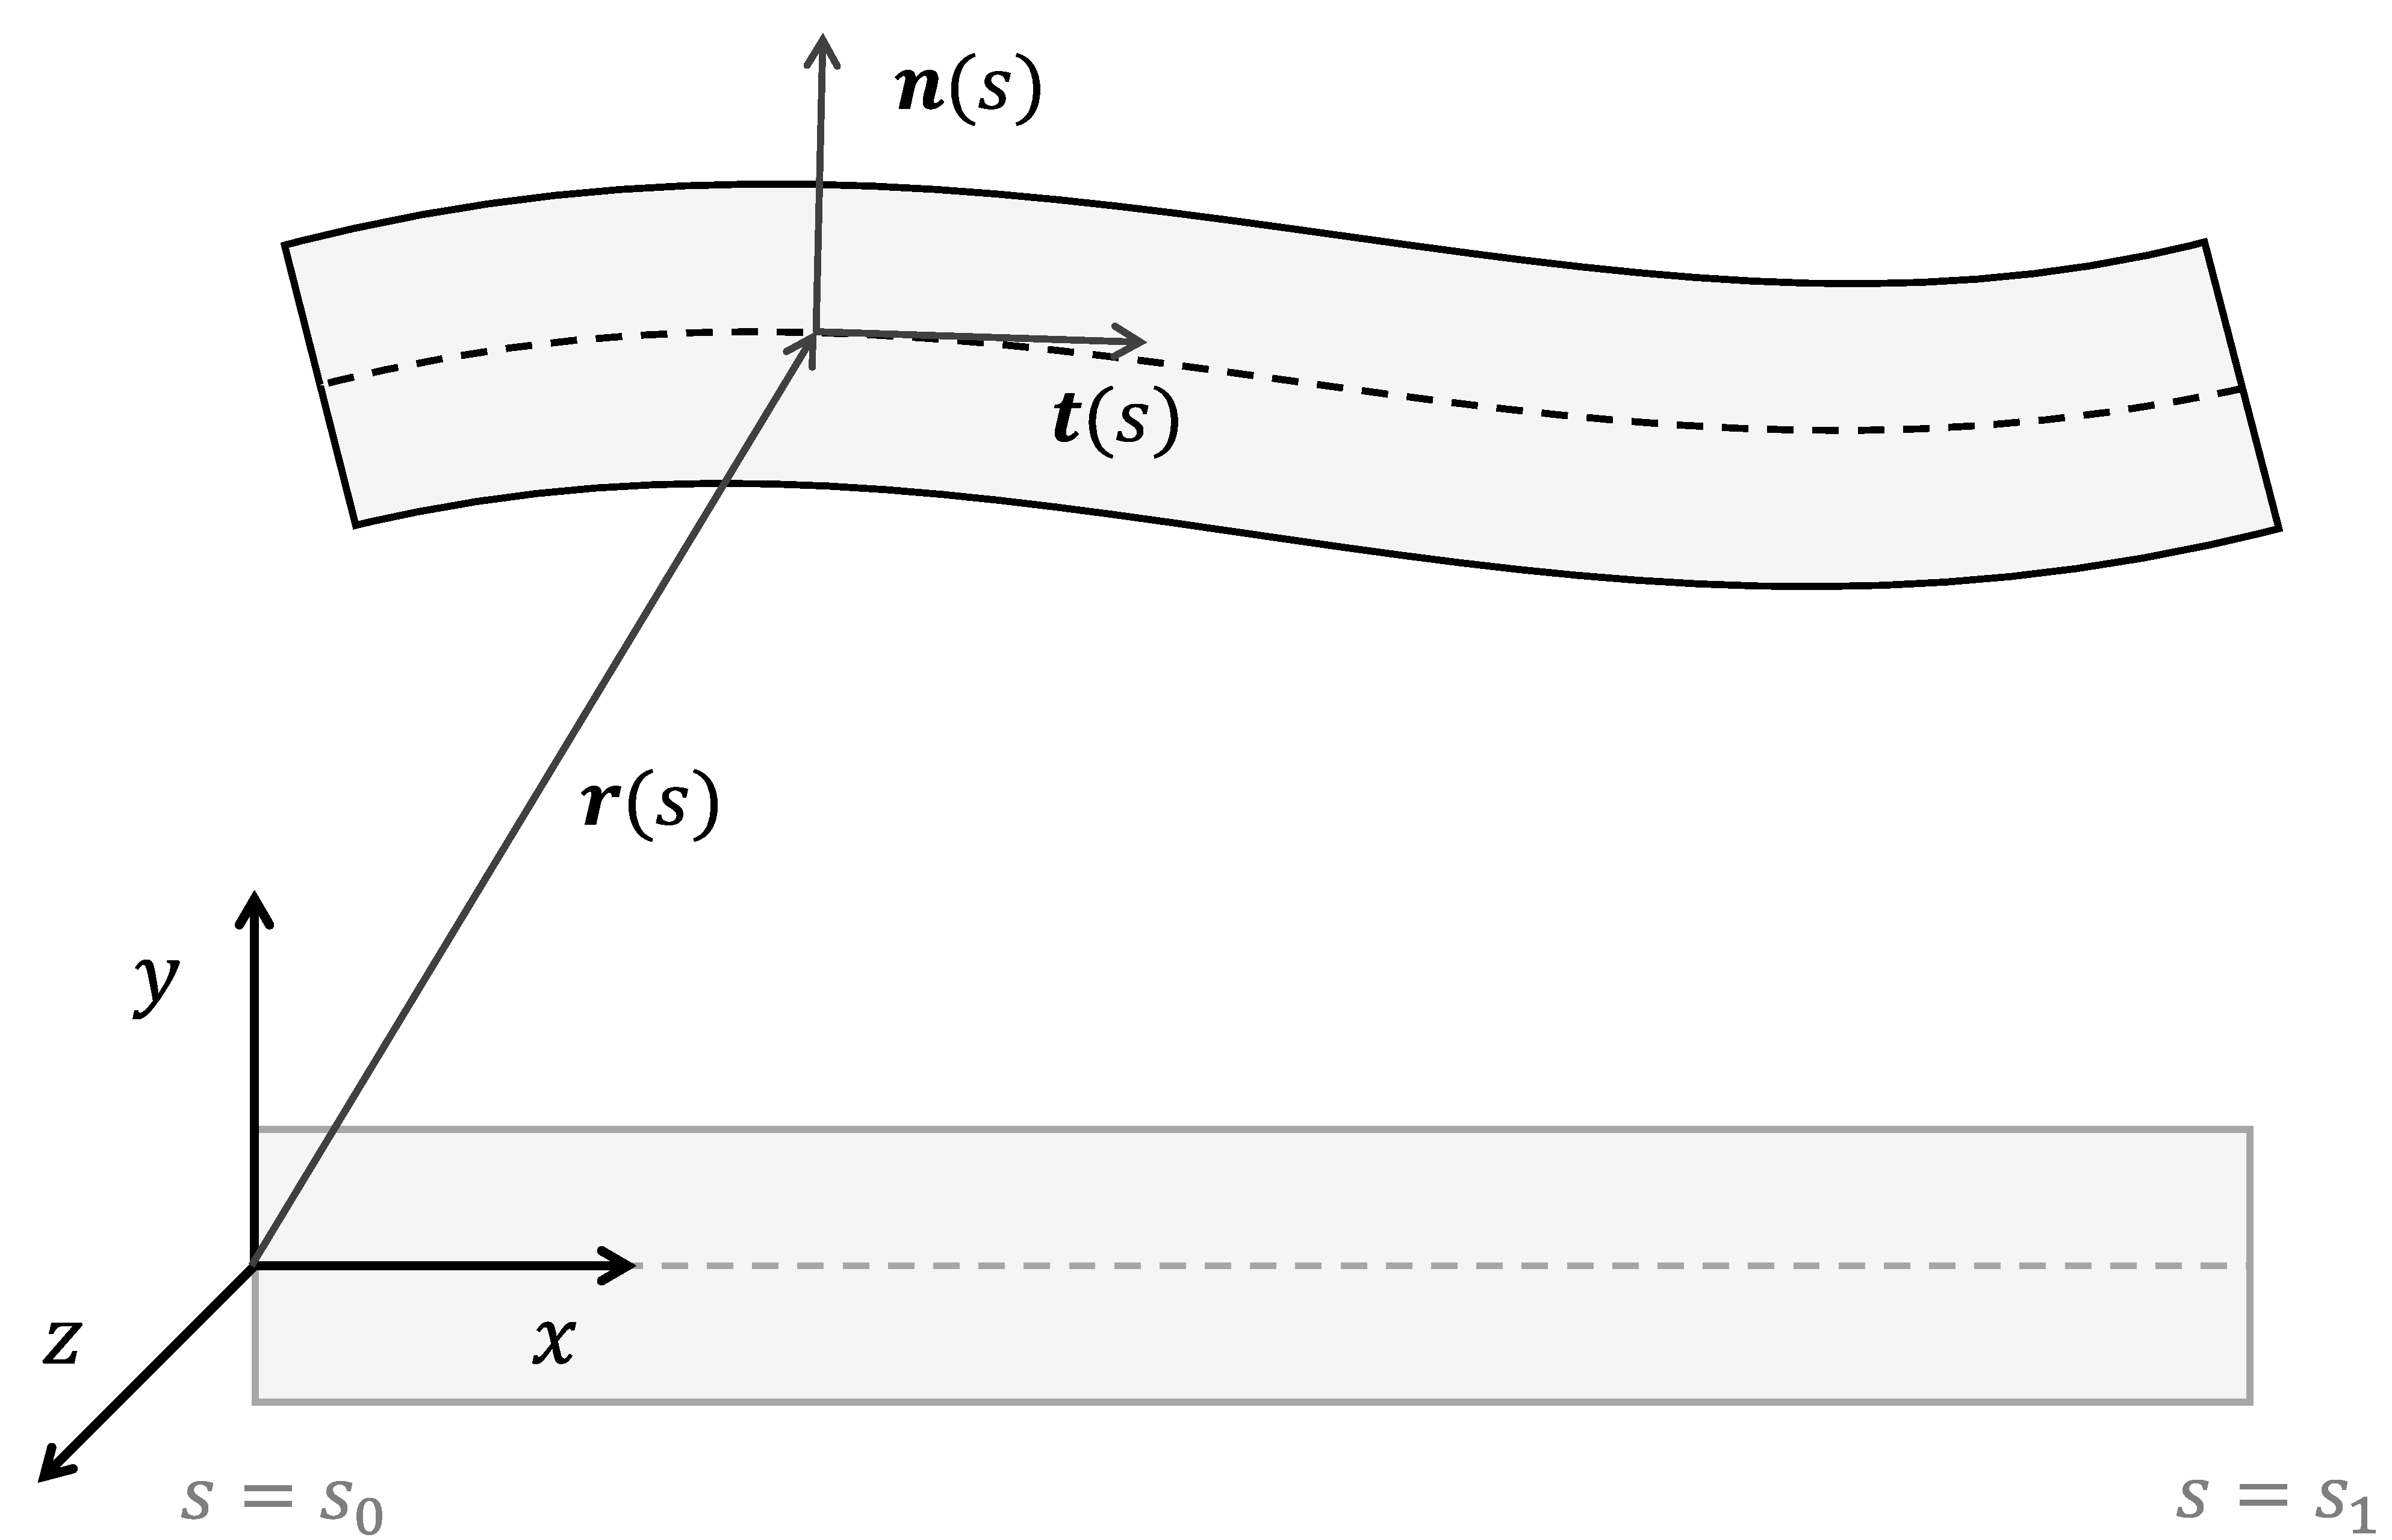
\includegraphics[width=0.6\textwidth]{figures/elements/beam-kinematics-referenceline}
\caption{Reference and deformed configuration of an initially straight beam}
\label{fig:beam-kinematics-referenceline}
\end{figure}

A second, deformed configuration is given by the function $\boldsymbol{r}(s)$, which maps the length~$s \in [s_{0},\,s_{1}]$ in the reference configuration to a corresponding point $\boldsymbol{r} \in \mathbb{R}^3$ on the deformed beam axis.
Since the beam is planar, this function only has nonzero components in the $x$ and $y$ directions and is zero in $z$,

\begin{equation}
\boldsymbol{r}(s) = \begin{bmatrix}
r_x(s) \\
r_y(s) \\
0
\end{bmatrix}.\label{eq:beam-axis-3d}
\end{equation}

It should be noted that the curve parameter $s$ only corresponds to a length in the reference configuration, it is not necessarily equal to the arc length along $\boldsymbol{r}(s)$.
For that curve it is only a general parameter.

Since the beam is supposed to be an Euler-Bernoulli beam, its cross sections are always perpendicular to the beam axis.
To express this geometrical constraint, we construct the local coordinate system $\{\boldsymbol{t},\,\boldsymbol{n},\,\boldsymbol{b}\}$ at the curve parameter $s$ as shown in figure~\ref{fig:beam-kinematics-crosssection}.

\begin{figure}[h]
\centering
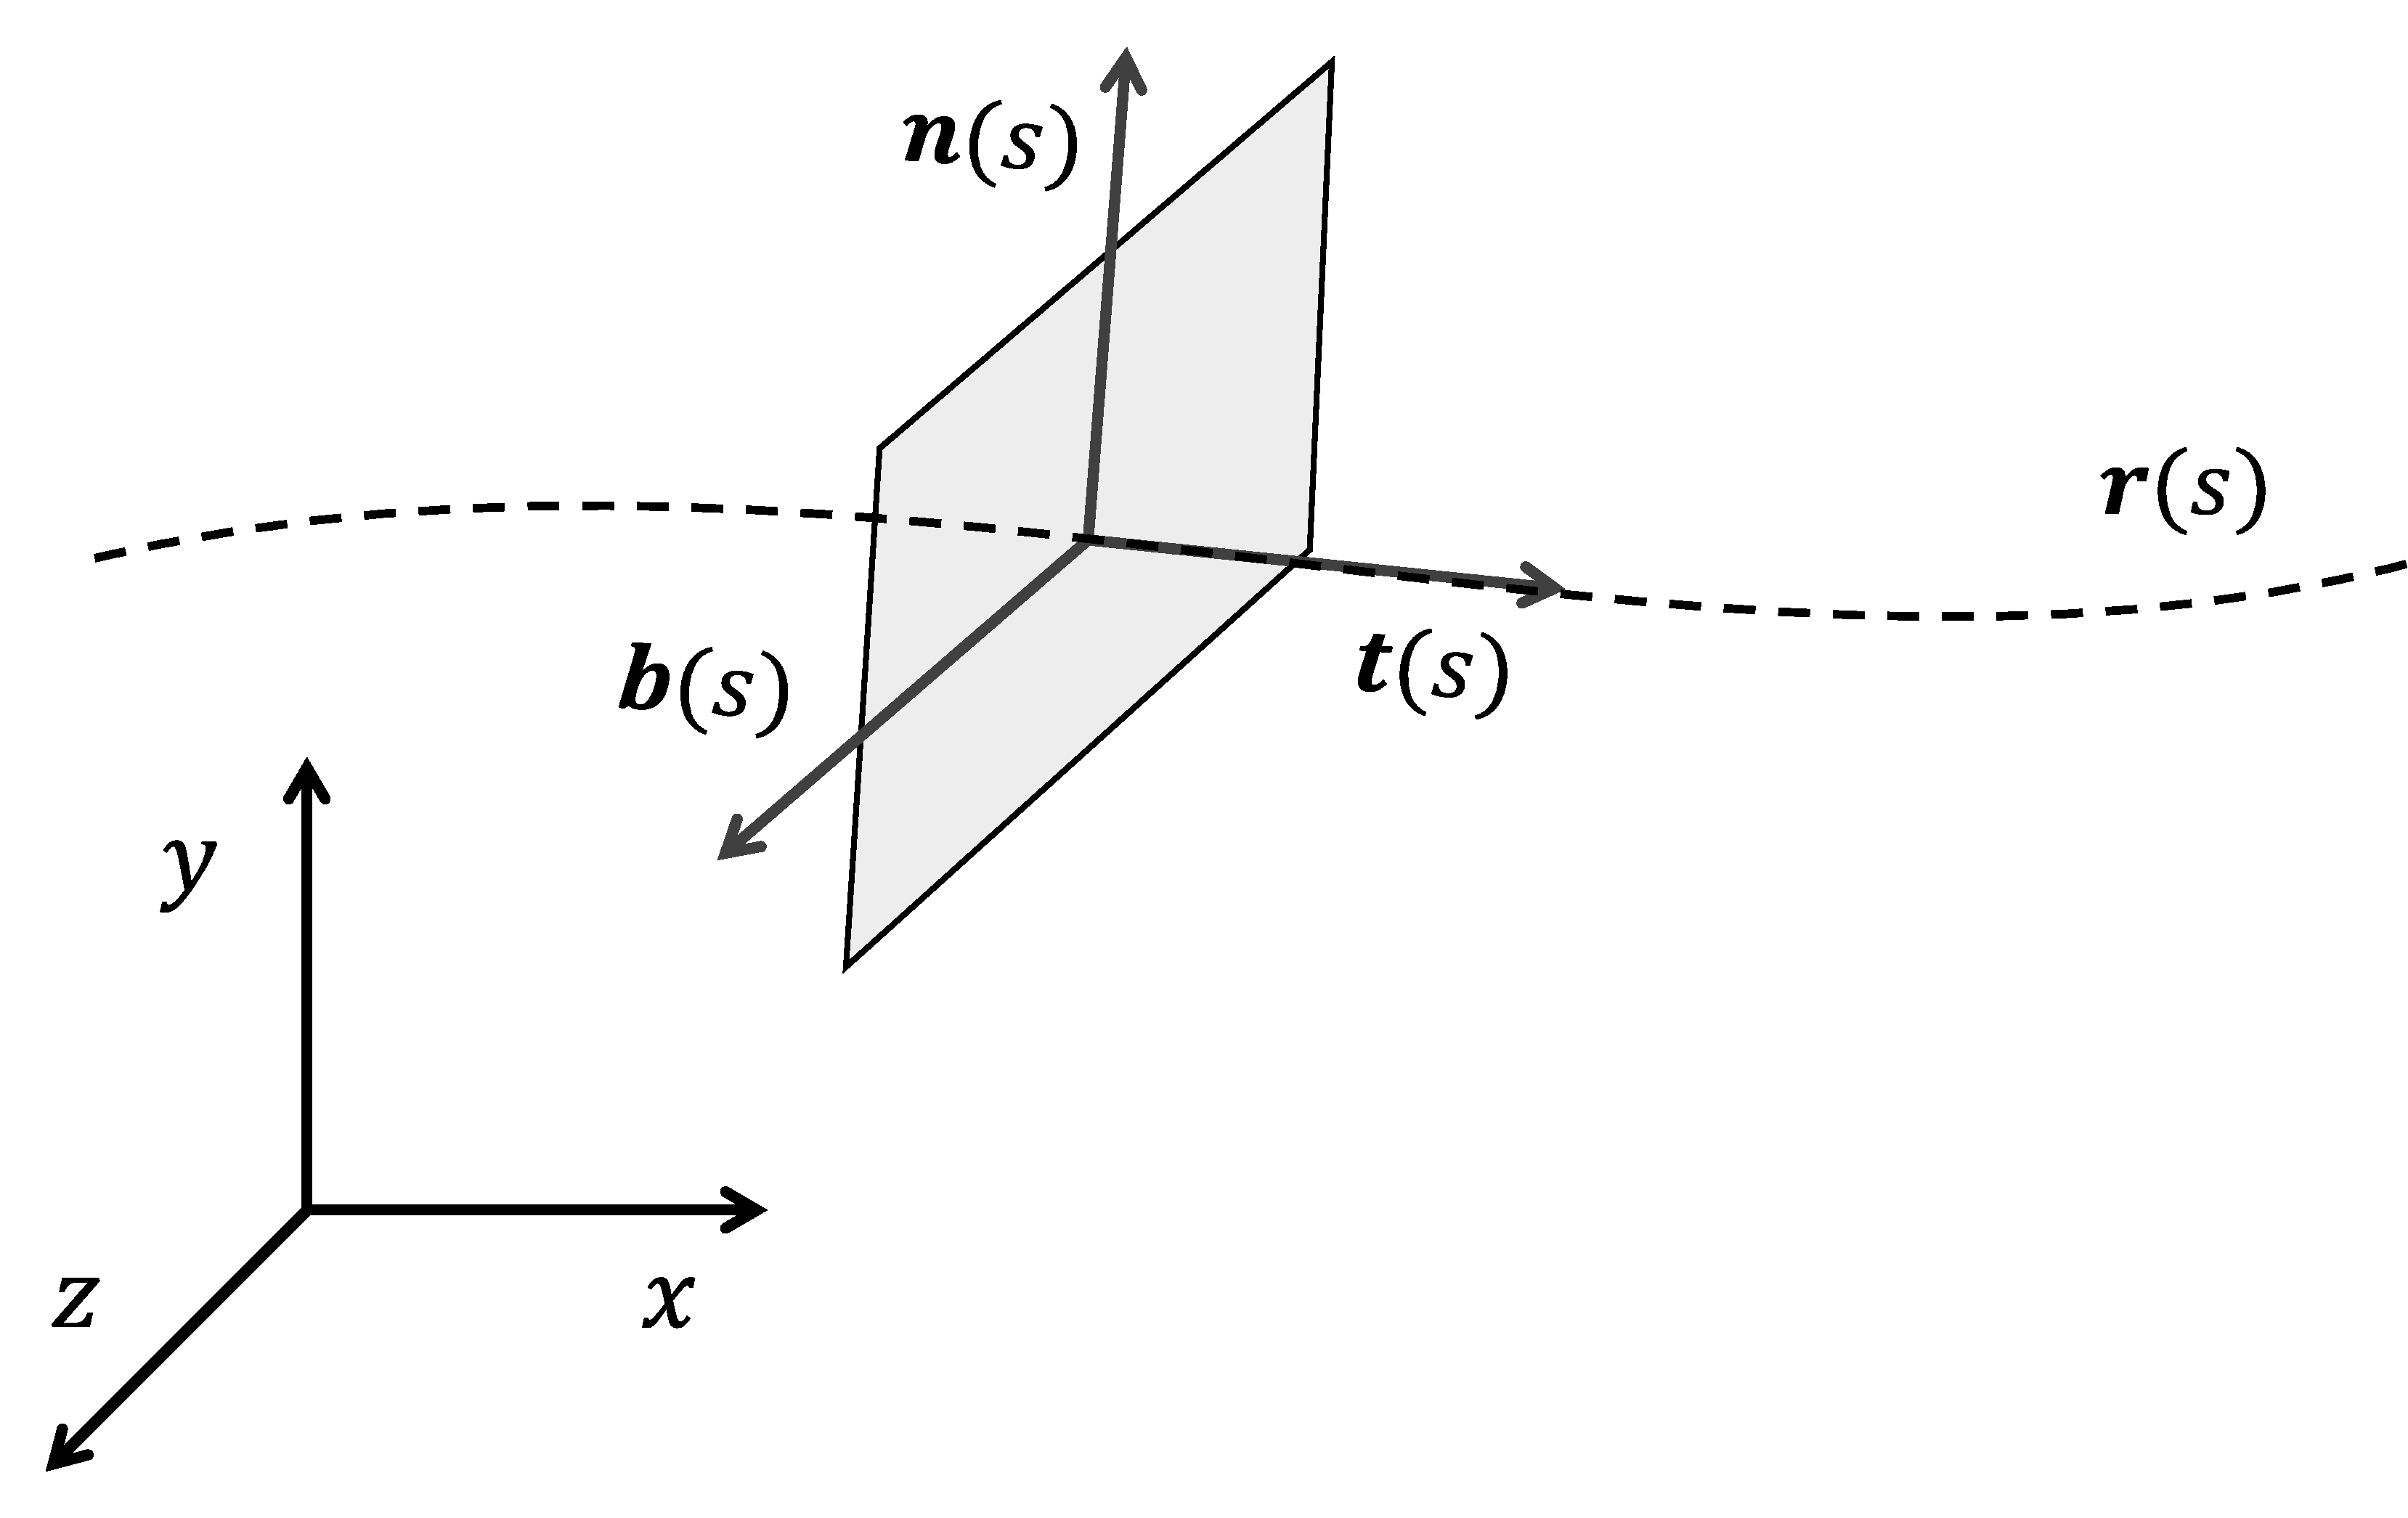
\includegraphics[width=0.5\textwidth]{figures/elements/beam-kinematics-crosssection}
\caption{Beam cross sections and attached coordinate system}
\label{fig:beam-kinematics-crosssection}
\end{figure}

The vector $\boldsymbol{t}(s)$ is the unit tangent vector of the curve, $\boldsymbol{n}(s)$ the unit normal vector and $\boldsymbol{b}(s)$ the unit binormal vector.
They can be expressed in terms of $\boldsymbol{r}(s)$ as

\begin{equation}
\boldsymbol{t}(s) = \frac{\boldsymbol{r}'(s)}{|\boldsymbol{r}'(s)|}, \quad \boldsymbol{n}(s) = \boldsymbol{b}(s) \times \boldsymbol{t}(s), \quad \boldsymbol{b}(s) = \boldsymbol{e}_{z}.
\end{equation}

With $\boldsymbol{e}_{z}$ being the unit vector in $z$ direction.
Since the cross sections are perpendicular to the beam axis and therefore to its tangent vector, they lie in the plane defined by $\boldsymbol{n}$ and $\boldsymbol{b}$.
With this information we can define a function $\boldsymbol{p}(x, y, z)$ that maps each material point $x, y, z$ in the cartesian reference coordinates to the corresponding point $\boldsymbol{p}$ in the deformed beam,

\begin{equation}
\boldsymbol{p}(x,y,z) = \boldsymbol{r}(x) + y\,\boldsymbol{n}(x) + z\,\boldsymbol{b}(x).
\end{equation}

This mapping is what's called a configuration in continuum mechanics terminology.
Another important concept from continuum mechanics that we are going to need is the so-called deformation gradient.
It is defined as the gradient/derivative of the mapping function $\boldsymbol{p}$ with respect to the cartesian reference coordinates,

\begin{align}
\boldsymbol{F} &= \begin{bmatrix}
\frac{\partial\boldsymbol{p}}{\partial x}, & \frac{\partial\boldsymbol{p}}{\partial y}, & \frac{\partial\boldsymbol{p}}{\partial z}
\end{bmatrix} \in \mathbb{R}^{3 \times 3}.
\end{align}

The deformation gradient characterizes the local deformation of the material points and is the basis for all sorts of strain and stress measures.
We can evaluate the required derivatives as

\begin{align}
\frac{\partial\boldsymbol{p}}{\partial x} &= \boldsymbol{r}'(x) + y\,\boldsymbol{n}'(x), \quad \frac{\partial\boldsymbol{p}}{\partial y} = \boldsymbol{n}(x), \quad \frac{\partial\boldsymbol{p}}{\partial z} = \boldsymbol{b}(x)
\end{align}

with the derivative of the normal direction with respect to the curve parameter being

\begin{align}
\boldsymbol{n}'(x) &= \boldsymbol{e}_{z} \times \boldsymbol{t}'(x) = \boldsymbol{e}_{z} \times \frac{\partial}{\partial x}\left(\frac{\boldsymbol{r}'}{|\boldsymbol{r}'|}\right) = \boldsymbol{e}_{z} \times \left(\frac{\boldsymbol{I}}{|\boldsymbol{r}'|} - \frac{\boldsymbol{r}'\boldsymbol{r}'^\intercal}{|\boldsymbol{r}'|^3}\right)\boldsymbol{r}'' \notag \\
&= \boldsymbol{e}_{z} \times \frac{\boldsymbol{r}''}{|\boldsymbol{r}'|} \quad\text{($\boldsymbol{r}'^\intercal\boldsymbol{r}'' = 0$ due to orthogonality)}.
\end{align}

% Source for some of the derivatives: The Matrix Cookbook (Kaare Brandt Petersen, Michael Syskind Pedersen)
% https://www.math.uwaterloo.ca/~hwolkowi/matrixcookbook.pdf

Like all square matrices, $\boldsymbol{F}$ can be written as the polar decomposition

\begin{equation}
\boldsymbol{F} = \boldsymbol{R}\,\boldsymbol{U} \label{eq:polar-decomposition}
\end{equation}

where $\boldsymbol{R} \in \mathbb{R}^{3 \times 3}$ is an orthonormal rotation matrix and $\boldsymbol{U} \in \mathbb{R}^{3 \times 3}$ is a symmetric and positive semi-definite stretch tensor.
Physically this can be interpreted as splitting the total deformation $\boldsymbol{F}$ into a pure rotation $\boldsymbol{R}$ and a pure scaling/stretch $\boldsymbol{U}$.
Fortunately we already know the rotational component of our deformation. It is given by the three basis vectors $\boldsymbol{t}$, $\boldsymbol{n}$ and $\boldsymbol{b}$ that are attached to the beam axis as

\begin{equation}
\boldsymbol{R} = \begin{bmatrix}
\boldsymbol{t}, & \boldsymbol{n}, & \boldsymbol{b}
\end{bmatrix}.
\end{equation}

Since we also know $\boldsymbol{F}$ from performing the required derivatives, we can compute the stretch tensor from equation (\ref{eq:polar-decomposition}) as

\begin{equation}
\boldsymbol{U} = \boldsymbol{R}^\intercal\,\boldsymbol{F} =
\begin{bmatrix}
\boldsymbol{t}^\intercal \\
\boldsymbol{n}^\intercal \\
\boldsymbol{b}^\intercal
\end{bmatrix}
\begin{bmatrix}
\frac{\partial\boldsymbol{p}}{\partial x}, & \frac{\partial\boldsymbol{p}}{\partial y}, & \frac{\partial\boldsymbol{p}}{\partial z}
\end{bmatrix}
=
\begin{bmatrix}
\boldsymbol{t}^\intercal\frac{\partial\boldsymbol{p}}{\partial x} & \boldsymbol{t}^\intercal\frac{\partial\boldsymbol{p}}{\partial y} & \boldsymbol{t}^\intercal\frac{\partial\boldsymbol{p}}{\partial z} \\
\\
\boldsymbol{n}^\intercal\frac{\partial\boldsymbol{p}}{\partial x} & \boldsymbol{n}^\intercal\frac{\partial\boldsymbol{p}}{\partial y} & \boldsymbol{n}^\intercal\frac{\partial\boldsymbol{p}}{\partial z} \\
\\
\boldsymbol{b}^\intercal\frac{\partial\boldsymbol{p}}{\partial x} & \boldsymbol{b}^\intercal\frac{\partial\boldsymbol{p}}{\partial y} & \boldsymbol{b}^\intercal\frac{\partial\boldsymbol{p}}{\partial z}
\end{bmatrix}
\end{equation}

Note that because $\boldsymbol{R}$ is orthonormal, its transpose is equal to its inverse, which was used here.
Because $\boldsymbol{t}$, $\boldsymbol{n}$, $\boldsymbol{b}$ are orthogonal, their products with each other evaluate to $0$ while products of a vector with itself evauate to $1$.
This already simplifies the second and third column of the stretch tensor.
Since forthermore $\frac{\partial\boldsymbol{p}}{\partial x}$ has the same direction as $\boldsymbol{t}$, only a single entry $U_{xx}$ of the stretch tensor that is not $0$ or $1$ remains,

\begin{equation}
\boldsymbol{U} =
\begin{bmatrix}
\boldsymbol{t}^\intercal\frac{\partial\boldsymbol{p}}{\partial x} & \boldsymbol{t}^\intercal\boldsymbol{n} & \boldsymbol{t}^\intercal\boldsymbol{b} \\
\\
\boldsymbol{n}^\intercal\frac{\partial\boldsymbol{p}}{\partial x} & \boldsymbol{n}^\intercal\boldsymbol{n} & \boldsymbol{n}^\intercal\boldsymbol{b} \\
\\
\boldsymbol{b}^\intercal\frac{\partial\boldsymbol{p}}{\partial x} & \boldsymbol{b}^\intercal\boldsymbol{n} & \boldsymbol{b}^\intercal\boldsymbol{b}
\end{bmatrix}
 =
\begin{bmatrix}
\boldsymbol{t}^\intercal\frac{\partial\boldsymbol{p}}{\partial x} & 0 & 0 \\
\\
\boldsymbol{n}^\intercal\frac{\partial\boldsymbol{p}}{\partial x} & 1 & 0 \\
\\
\boldsymbol{b}^\intercal\frac{\partial\boldsymbol{p}}{\partial x} & 0 & 1
\end{bmatrix}
=
\begin{bmatrix}
\boldsymbol{t}^\intercal\frac{\partial\boldsymbol{p}}{\partial x} & 0 & 0 \\
\\
0 & 1 & 0 \\
\\
0 & 0 & 1
\end{bmatrix}.
\end{equation}

It can be evaluated as

\begin{align}
U_{xx} &= \boldsymbol{t}^\intercal\frac{\partial\boldsymbol{p}}{\partial x} = \boldsymbol{t}^\intercal\left(\boldsymbol{r}' + y\,\boldsymbol{n}'\right) = \boldsymbol{t}^\intercal\left(\boldsymbol{r}' + y\left(\boldsymbol{e}_{z} \times \frac{\boldsymbol{r}''}{|\boldsymbol{r}'|}\right)\right) \notag \\
&= \frac{\boldsymbol{r}'^\intercal\boldsymbol{r}'}{|\boldsymbol{r}'|} + y\, \frac{\boldsymbol{r}'^\intercal}{|\boldsymbol{r}'|}\left(\boldsymbol{e}_{z} \times \frac{\boldsymbol{r}''}{|\boldsymbol{r}'|}\right) \notag \\
&= |\boldsymbol{r}'| - y\,\boldsymbol{e}_{z}^\intercal\left(\frac{\boldsymbol{r}' \times \boldsymbol{r}''}{|\boldsymbol{r}'|^2}\right)\label{eq:stretch-tensor-component}
\end{align}

Finally we use the definition of the Biot strain tensor $\boldsymbol{E} = \boldsymbol{U} - \boldsymbol{I}$ [source] to compute the material strains corresponding to our deformation.
It can easily be seen that the strain tensor only has a single nonzero component in the axial direction,

\begin{equation}
\varepsilon_{xx} = |\boldsymbol{r}'| - 1 - y\,\boldsymbol{e}_{z}^\intercal\left(\frac{\boldsymbol{r}' \times \boldsymbol{r}''}{|\boldsymbol{r}'|^2}\right). \label{eq:strain-over-section}
\end{equation}

This is the strain normal to our beam's cross sections.
It varies linearly over the height of the section ($y$ coordinate) but is constant over its width ($z$ coordinate).
By defining the quantities

\begin{equation}
\varepsilon = |\boldsymbol{r}'| - 1, \quad \kappa = \boldsymbol{e}_{z}^\intercal\left(\frac{\boldsymbol{r}' \times \boldsymbol{r}''}{|\boldsymbol{r}'|^2}\right),
\end{equation}

which are constant over a given cross section, we can write equation (\ref{eq:strain-over-section}) as

\begin{equation}
\varepsilon_{xx} = \varepsilon - y\,\kappa. \label{eq:strain-over-section}
\end{equation}

Here, $\varepsilon$ is the strain from elongation of the beam axis and $\kappa$ is a measure of its curvature.

Note however that $\kappa$ is not identical to the classical curvature, which is expressed as $\frac{|\boldsymbol{r}' \times \boldsymbol{r}''|}{|\boldsymbol{r}'|^3}$.
First because $\kappa$ is signed, i.e. can be positive or negative, but more importantly because it differs by a factor of $|\boldsymbol{r}'|$.
This distinction is outlined in great detail in [gerstmayr], where the term \textit{material measure of curvature} is introduced.
For simplicity we will just call $\kappa$ the curvature, but what we actually mean is the material measure of curvature.

\subsection{Undeformed state}

In the previous section, the axial strain $\varepsilon_{xx}$ for a beam with an initially straight reference configuration was derived.
Now we will extend this to beams that are not straight in their undeformed state.

\begin{figure}[h]
\centering
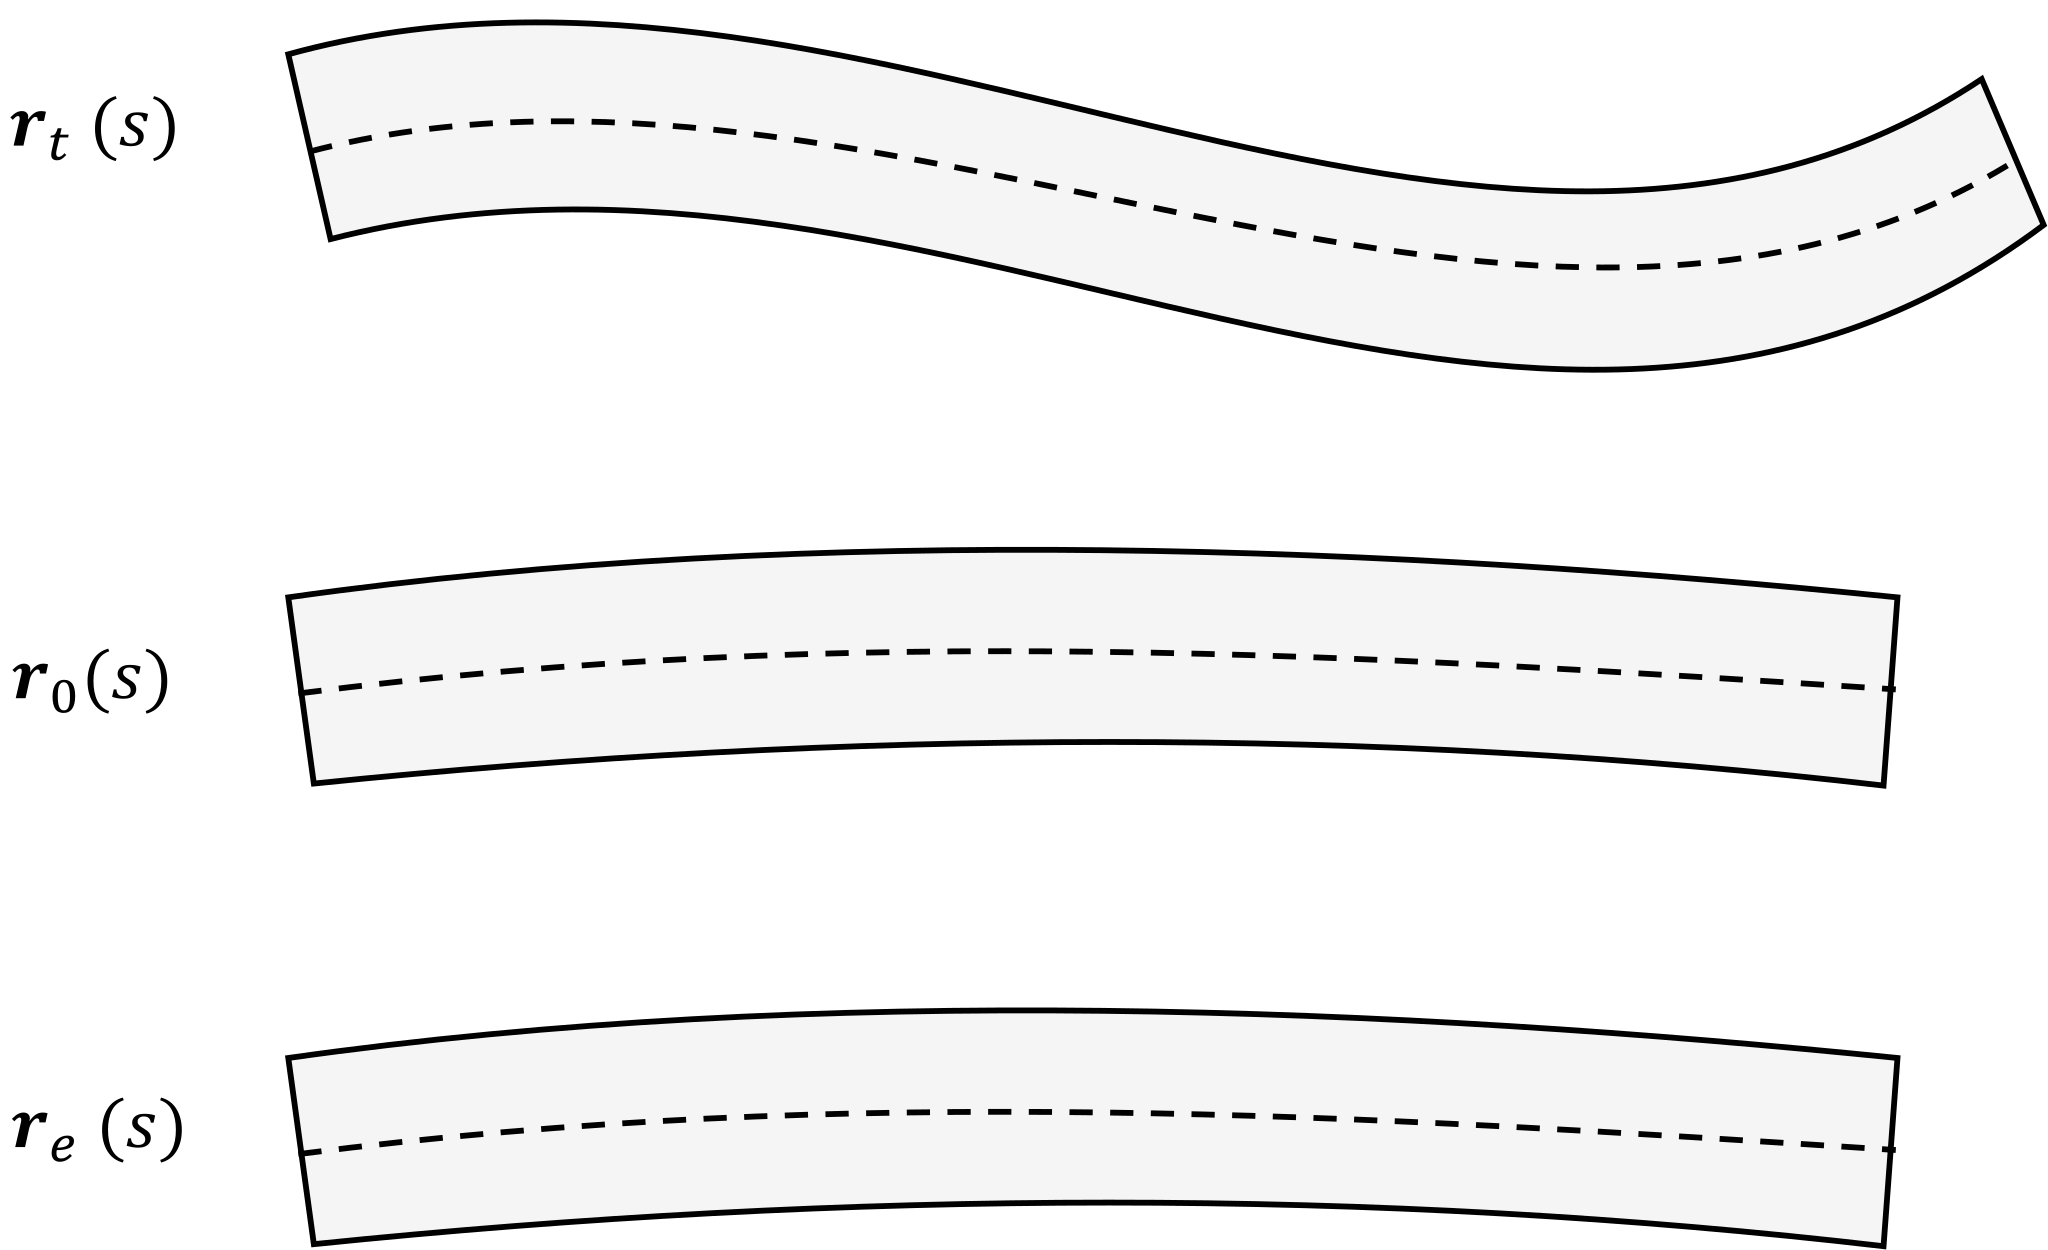
\includegraphics[width=0.5\textwidth]{figures/elements/beam-kinematics-configurations}
\caption{Beam configurations}
\label{fig:beam-kinematics-configurations}
\end{figure}

For this, we will consider three different configurations of the beam:

\begin{itemize}
\item \textbf{Exact geometry} $\boldsymbol{p}_{e}$: This is the exact initial geometry of the beam as defined by the bow model. If the user defined it to be a circular arc for example, it is exactly that.

\item \textbf{Undeformed geometry} $\boldsymbol{p}_{0}$: This is the initial geometry of the beam at time $t = 0$ as approximated by the finite element's shape functions. It might not match the exact geometry exactly, because polynomial shape functions for example can't represent a circular arc without a small error.

\item \textbf{Deformed geometry} $\boldsymbol{p}_{t}$: This is the deformed geometry of the beam at time $t \ge 0$ as approximated by the finite element's shape functions.
\end{itemize}

The deformation we want to measure is the one between the undeformed approximation $\boldsymbol{p}_{0}$ and the deformed approximation $\boldsymbol{p}_{t}$.
What we already derived earlier are the deformation gradients of each of those configurations with respect to an initially straight configuration,

\begin{equation}
\boldsymbol{F}_{e} = \frac{\partial \boldsymbol{p}_{e}}{\partial \boldsymbol{x}}, \quad \boldsymbol{F}_{0} = \frac{\partial \boldsymbol{p}_{0}}{\partial \boldsymbol{x}}, \quad \boldsymbol{F}_{t} = \frac{\partial \boldsymbol{p}_{t}}{\partial \boldsymbol{x}}
\end{equation}

From those, the deformation gradient between the two configurations in question can be obtained by using the chain rule,

\begin{equation}
\boldsymbol{F} = \frac{\partial \boldsymbol{p}_{t}}{\partial \boldsymbol{p}_{0}} = \frac{\partial \boldsymbol{p}_{t}}{\partial \boldsymbol{x}}\frac{\partial \boldsymbol{x}}{\partial \boldsymbol{p}_{0}} = \boldsymbol{F}_{t}\,\boldsymbol{F}_{0}^{-1}.
\end{equation}

The tensors on the right hand side already have the known polar decompositions $\boldsymbol{F}_{0} = \boldsymbol{R}_{0}\,\boldsymbol{U}_{0}$ and $\boldsymbol{F}_{t} = \boldsymbol{R}_{t}\,\boldsymbol{U}_{t}$.
For the left hand side, we can work out that the relative rotation between the configurations is $\boldsymbol{R} = \boldsymbol{R}_{0}^\intercal\,\boldsymbol{R}_{t}$.
Furthermore, all the rotation matrices describe rotations around the same axis ($z$) and are therefore commutative, i.e. their order of multiplication doesn't matter.
Using all this, the relative stretch tensor can be derived as

\begin{align}
\boldsymbol{F} &= \boldsymbol{F}_{t}\,\boldsymbol{F}_{0}^{-1} \notag \\
\boldsymbol{R}\,\boldsymbol{U} &= \boldsymbol{R}_{t}\,\boldsymbol{U}_{t}\left(\boldsymbol{R}_{0}\,\boldsymbol{U}_{0}\right)^{-1} \notag \\
\boldsymbol{R}_{0}^\intercal\,\boldsymbol{R}_{t}\,\boldsymbol{U} &= \boldsymbol{R}_{t}\,\boldsymbol{U}_{t}\,\boldsymbol{U}_{0}^{-1}\,\boldsymbol{R}_{0}^\intercal \notag \\
\boldsymbol{U} &= \boldsymbol{U}_{t}\,\boldsymbol{U}_{0}^{-1}
\end{align}

Luckily for us the involved stretch tensors are diagonaol, so that carrying out the matrix inversion and multiplication results in a simple division.
The result for the axial stretch is therefore

\begin{equation}
U_{xx} = \frac{U_{xx}^{t}}{U_{xx}^{0}} = \frac{|\boldsymbol{r}_{t}'| - y\kappa_{t}}{|\boldsymbol{r}_{0}'| - y\kappa_{0}}. \label{eq:strain-nonlinear}
\end{equation}

This is a rational function in $y$ as opposed to the linear function we got before and confirms the known result that the strain in a pre-curved Euler-Bernoulli beam is in general no longer linearly distributed over the cross section height.
This is a known result [source?] and there are ways to account for it when it matters, i.e. when the height of the cross sections is significant compared to the radius of curvature [source: winkler curved beam approximation].

For our purposes however we can assume the beam to be thin and only moderately curved compared to its cross section height.
This allows us to linearize the strain expression (\ref{eq:strain-nonlinear}) in order to arrive at something that more closely resembles classical Euler-Bernoulli beam theory.

Linearizing $U_{xx}(y)$ around $y = 0$ yields the simplified axial stretch

\begin{align}
U_{xx}(y) &\approx U_{xx}(0) + y\,U_{xx}'(0) \notag \\
\notag \\
&\approx \left[\frac{|\boldsymbol{r}_{t}'| - y\kappa_{t}}{|\boldsymbol{r}_{0}'| - y\kappa_{0}}\right]_{y=0} + y\left[\frac{-(|\boldsymbol{r}_{0}'| - y\kappa_{0})\kappa_{t} + (|\boldsymbol{r}_{t}'| - y\kappa_{t})\kappa_{0}}{(|\boldsymbol{r}_{0}'| - y\kappa_{0})^2}\right]_{y=0} \notag \\
\notag \\
&\approx \frac{|\boldsymbol{r}_{t}'|}{|\boldsymbol{r}_{0}'|} - y\,\frac{|\boldsymbol{r}_{0}'|\kappa_{t} - |\boldsymbol{r}_{t}'|\kappa_{0}}{|\boldsymbol{r}_{0}'|^2}
\end{align}

from which the corresponding Biot strain $\varepsilon_{xx} = U_{xx} - 1$ follows as

\begin{equation}
\varepsilon_{xx} = \frac{|\boldsymbol{r}_{t}'|}{|\boldsymbol{r}_{0}'|} - 1 - y\,\frac{|\boldsymbol{r}_{0}'|\kappa_{t} - |\boldsymbol{r}_{t}'|\kappa_{0}}{|\boldsymbol{r}_{0}'|^2}. \label{eq:axial-strain-predeformed}
\end{equation}

This now has the same structure~$\varepsilon_{xx} = \varepsilon - y\kappa$ as the strain expression we derived before in equation (\ref{eq:strain-over-section}), but with modified expressions for the axial strain~$\varepsilon$ and the curvature~$\kappa$,

\begin{equation}
\varepsilon = \frac{|\boldsymbol{r}_{t}'|}{|\boldsymbol{r}_{0}'|} - 1, \quad \kappa = \frac{|\boldsymbol{r}_{0}'|\kappa_{t} - |\boldsymbol{r}_{t}'|\kappa_{0}}{|\boldsymbol{r}_{0}'|^2}.
\end{equation}

Since I haven't been able to find any source that arrives at identical expressions for a predeformed planar beam so far (although [curvature-constrained-interpolation-method] comes close), some simple plausibility checks are in order.

\subsection{Plausibility checks}

\subsubsection{Bar with constant strain}

To verify the plausibility of the axial strain, consider a straight bar as shown in figure \ref{fig:beam-kinematics-verification-1}.
It has a length of $l$ in the exact reference configuration, a length of $l_{0}$ in the undeformed configuration and of $l_{t}$ in the deformed configuration.

\begin{figure}[h]
\centering
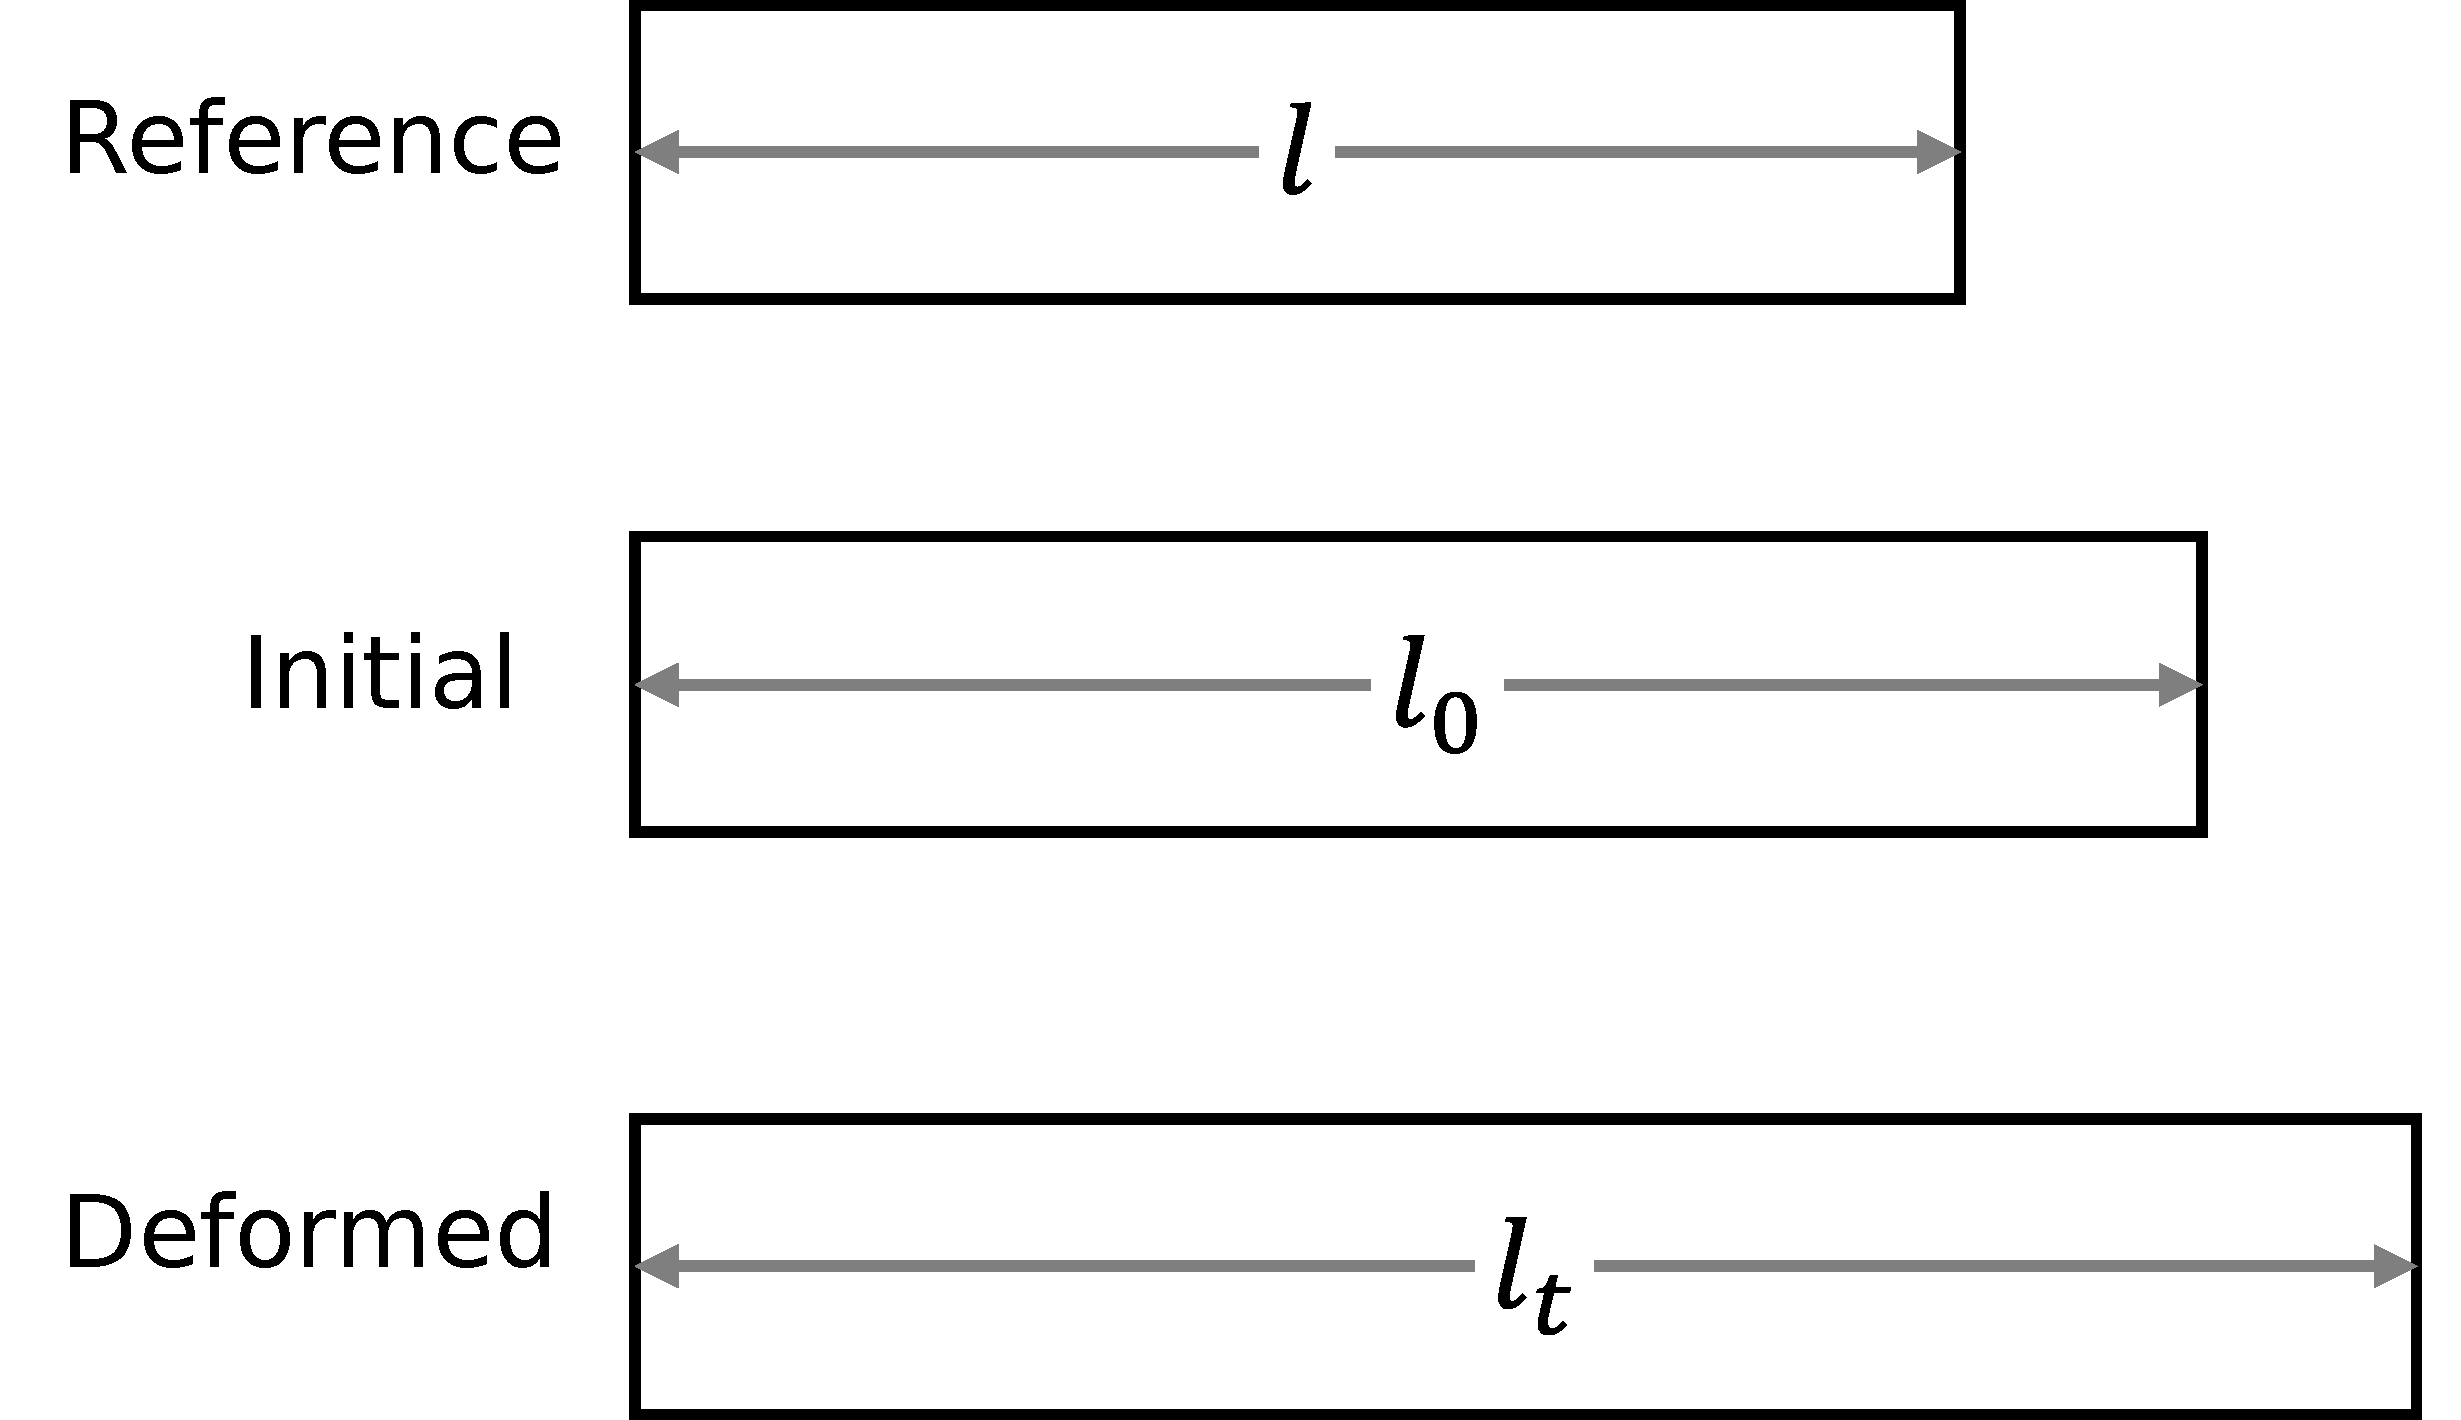
\includegraphics[width=0.5\textwidth]{figures/elements/beam-kinematics-verification-1}
\caption{Straight bar in three configurations}
\label{fig:beam-kinematics-verification-1}
\end{figure}

Assuming constant strain over the length of the bar, we can express the strain between the undeformed and deformed states by simple geometrical consideration as

\begin{equation}
\varepsilon_{xx} = \frac{l_{t} - l_{0}}{l_{0}} = \frac{l_{t}}{l_{0}} - 1.
\end{equation}

So this is what our strain expression should also evaluate to.
If we apply (\ref{eq:axial-strain-predeformed}) to this example we get

\begin{equation}
\varepsilon_{xx} = \frac{|\boldsymbol{r}_{t}'|}{|\boldsymbol{r}_{0}'|} - 1 = \frac{l_{t}/l}{l_{0}/l} - 1 = \frac{l_{t}}{l_{0}} - 1.
\end{equation}

Both results are indeed identical, so our expression passes this check.

\subsubsection{Beam with constant strain and curvature}

For the curvature expression, consider the circular arc shown in figure \ref{fig:beam-kinematics-verification-3}.
In undeformed state, the length of the beam axis is $l_{0}$ and its radius of curvature is $R_{0}$.
In deformed state, the length and radius are $l_{t}$ and $R_{t}$, respectively.

\begin{figure}[h]
\centering
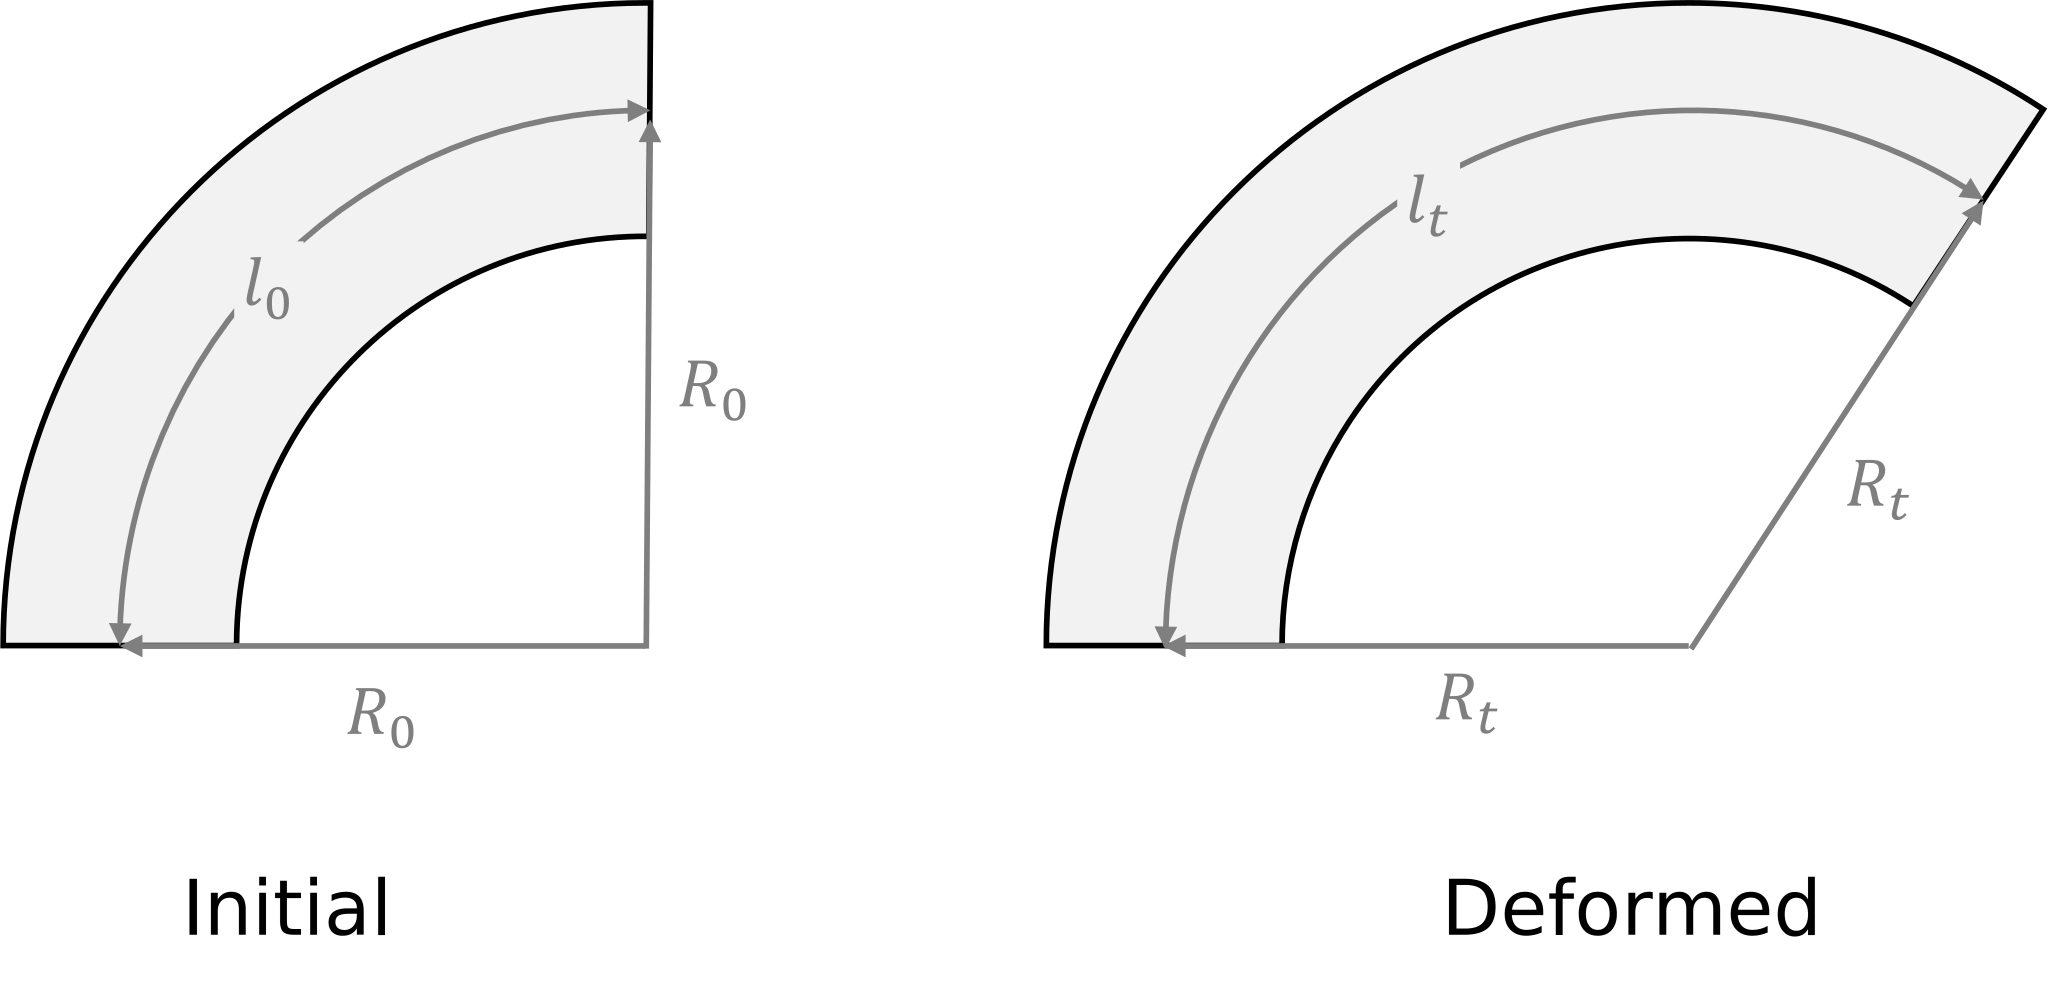
\includegraphics[width=0.5\textwidth]{figures/elements/beam-kinematics-verification-2}
\caption{Beam with constant strain and curvature}
\label{fig:beam-kinematics-verification-2}
\end{figure}

Like before, we first develop a result for the strain by geometrical considerations.
In both configurations we can develop a relationship between the distance $y$ from the centerline of the beam axis and the resulting length $l^y$ of a fiber in the beam.

\begin{figure}[h]
\centering
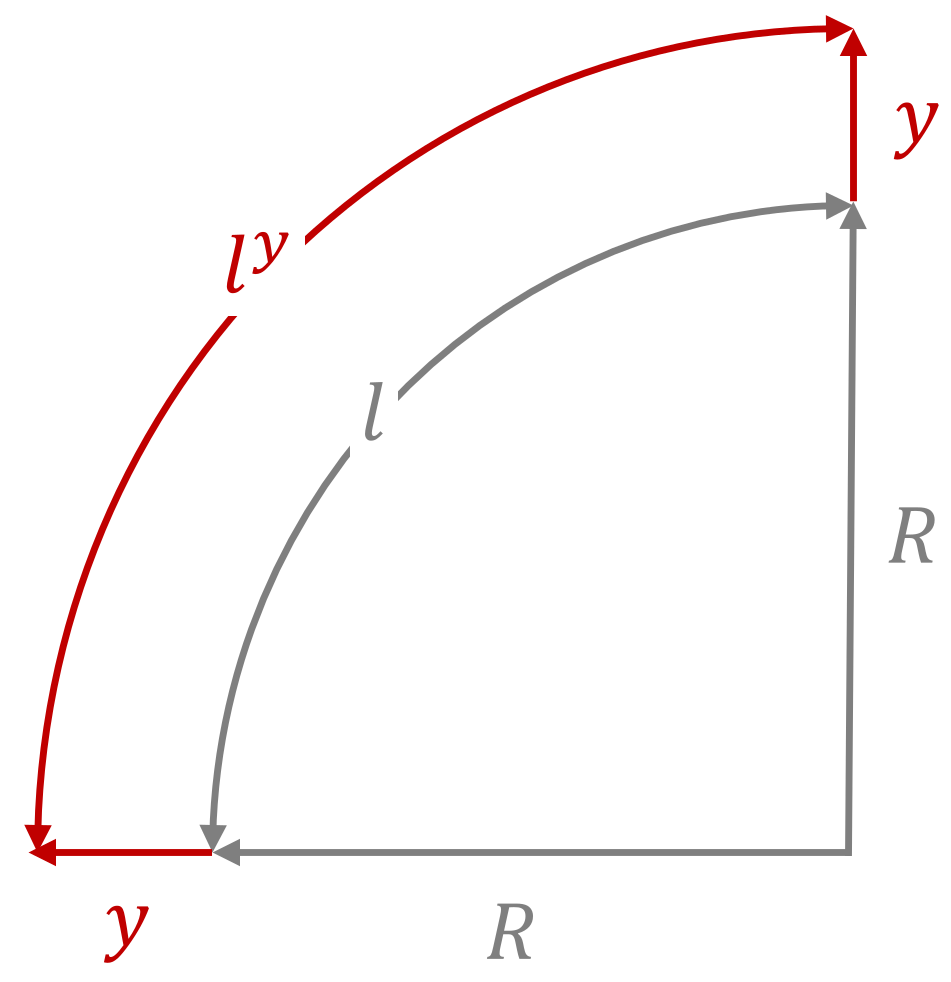
\includegraphics[width=0.25\textwidth]{figures/elements/beam-kinematics-verification-3}
\caption{Length of a fiber in the beam}
\label{fig:beam-kinematics-verification-3}
\end{figure}

With the help of figure \ref{fig:beam-kinematics-verification-3} we can formulate the following relationship,

\begin{equation}
\frac{l}{R} = \frac{l^y}{y + R} \ \Rightarrow\ l^y = \frac{l}{R}(y + R).
\end{equation}

This directly gives us the strain as a relation between lengths in undeformed and deformed states,

\begin{equation}
\varepsilon_{xx}(y) = \frac{l_t^y - l_0^y}{l_0^y} = \frac{l_t^y}{l_0^y} - 1 = \frac{\frac{l_t}{R_t}(y + R_t)}{\frac{l_0}{R_0}(y + R_0)} - 1
\end{equation}

This is nonlinear in $y$, just like the intermediate result (\ref{eq:strain-nonlinear}) was before and it can be verified that those two are already identical.
But to be completely sure we carry out the linearization, which results in

\begin{align}
\varepsilon_{xx}(y) &\approx \varepsilon_{xx}(0) + y\,\varepsilon_{xx}'(0) \notag \\
\notag \\
&\approx \left[\frac{\frac{l_t}{R_t}(y + R_t)}{\frac{l_0}{R_0}(y + R_0)} - 1\right]_{y=0} + y\,\left[\frac{\frac{l_0 l_t}{R_0 R_t}(y + R_0) - \frac{l_0 l_t}{R_0 R_t}(y + R_t)}{\frac{l_0^2}{R_0^2}(y + R_0)^2}\right]_{y=0} \notag \\
\notag \\
&\approx \frac{l_t}{l_0} - 1 + y\,\frac{l_t}{l_0}\left(\frac{1}{R_t} - \frac{1}{R_0}\right). \notag \\
\end{align}

For comparison we evaluate equation (\ref{eq:axial-strain-predeformed}) for the setup.
Some care must be taken with the sign of the curvature and the difference between the geometrical curvature, which would be $\frac{1}{R}$, and the material measure of curvature that is actually needed.

\begin{align}
|\boldsymbol{r}_{0}'| &= \frac{l_{0}}{l} \quad \kappa_{0} = -\frac{|\boldsymbol{r}_{0}'|}{R_{0}} = -\frac{l_{0}}{lR_{0}} \\
|\boldsymbol{r}_{t}'| &= \frac{l_{t}}{l} \quad \kappa_{t} = -\frac{|\boldsymbol{r}_{t}'|}{R_{t}} = -\frac{l_{t}}{lR_{t}} \\
\notag \\
\varepsilon_{xx} &= \frac{|\boldsymbol{r}_{t}'|}{|\boldsymbol{r}_{0}'|} - 1 - y\,\frac{|\boldsymbol{r}_{0}'|\kappa_{t} - |\boldsymbol{r}_{t}'|\kappa_{0}}{|\boldsymbol{r}_{0}'|^2} = \frac{l_{t}}{l_{0}} - 1 + y\,\frac{\frac{l_0 l_t}{l^2 R_t} - \frac{l_t l_0}{l^2 R_0}}{\frac{l_0^2}{l^2}} \notag \\
&= \frac{l_t}{l_0} - 1 + y\,\frac{l_t}{l_0}\left(\frac{1}{R_t} - \frac{1}{R_0}\right).
\end{align}

This is again the same result as that from the geometric derivation, so out strain expression passes this check too.

\newpage
\subsection{Absolute nodal coordinate formulation}

In order to construct a finite element for the discussed beam, we have to pick a finite set of coordinates in which we want to describe its motion and interpolate the continuous quantities within the beam in terms of those coordinates.
Usually the element is given a set of nodes and the coordinates consist of some kinematic quantities at those nodes that describe their position and/or orientation.

For a planar beam element with two nodes, for example, a natural choice of coordinates might be the positions of the nodes as well as the orientation angle of the beam at each node.
These approaches however lead to the problem of interpolating both positions and rotations in a consistent way and also result in a non-constant mass matrix that depends on the nodal coordinates in a nonlinear way.

This is where the absolute nodal coordinate formulation (ANCF), first proposed by Shabana [source], comes into play.
This method uses the slopes/gradient vectors $\boldsymbol{r}'$ of the beam axis to describe the orientation of the nodes, leading to some nice properties of the element, like a constant mass matrix, and avoiding some of the possible complications associated with rotation angles.

\begin{figure}[h]
\centering
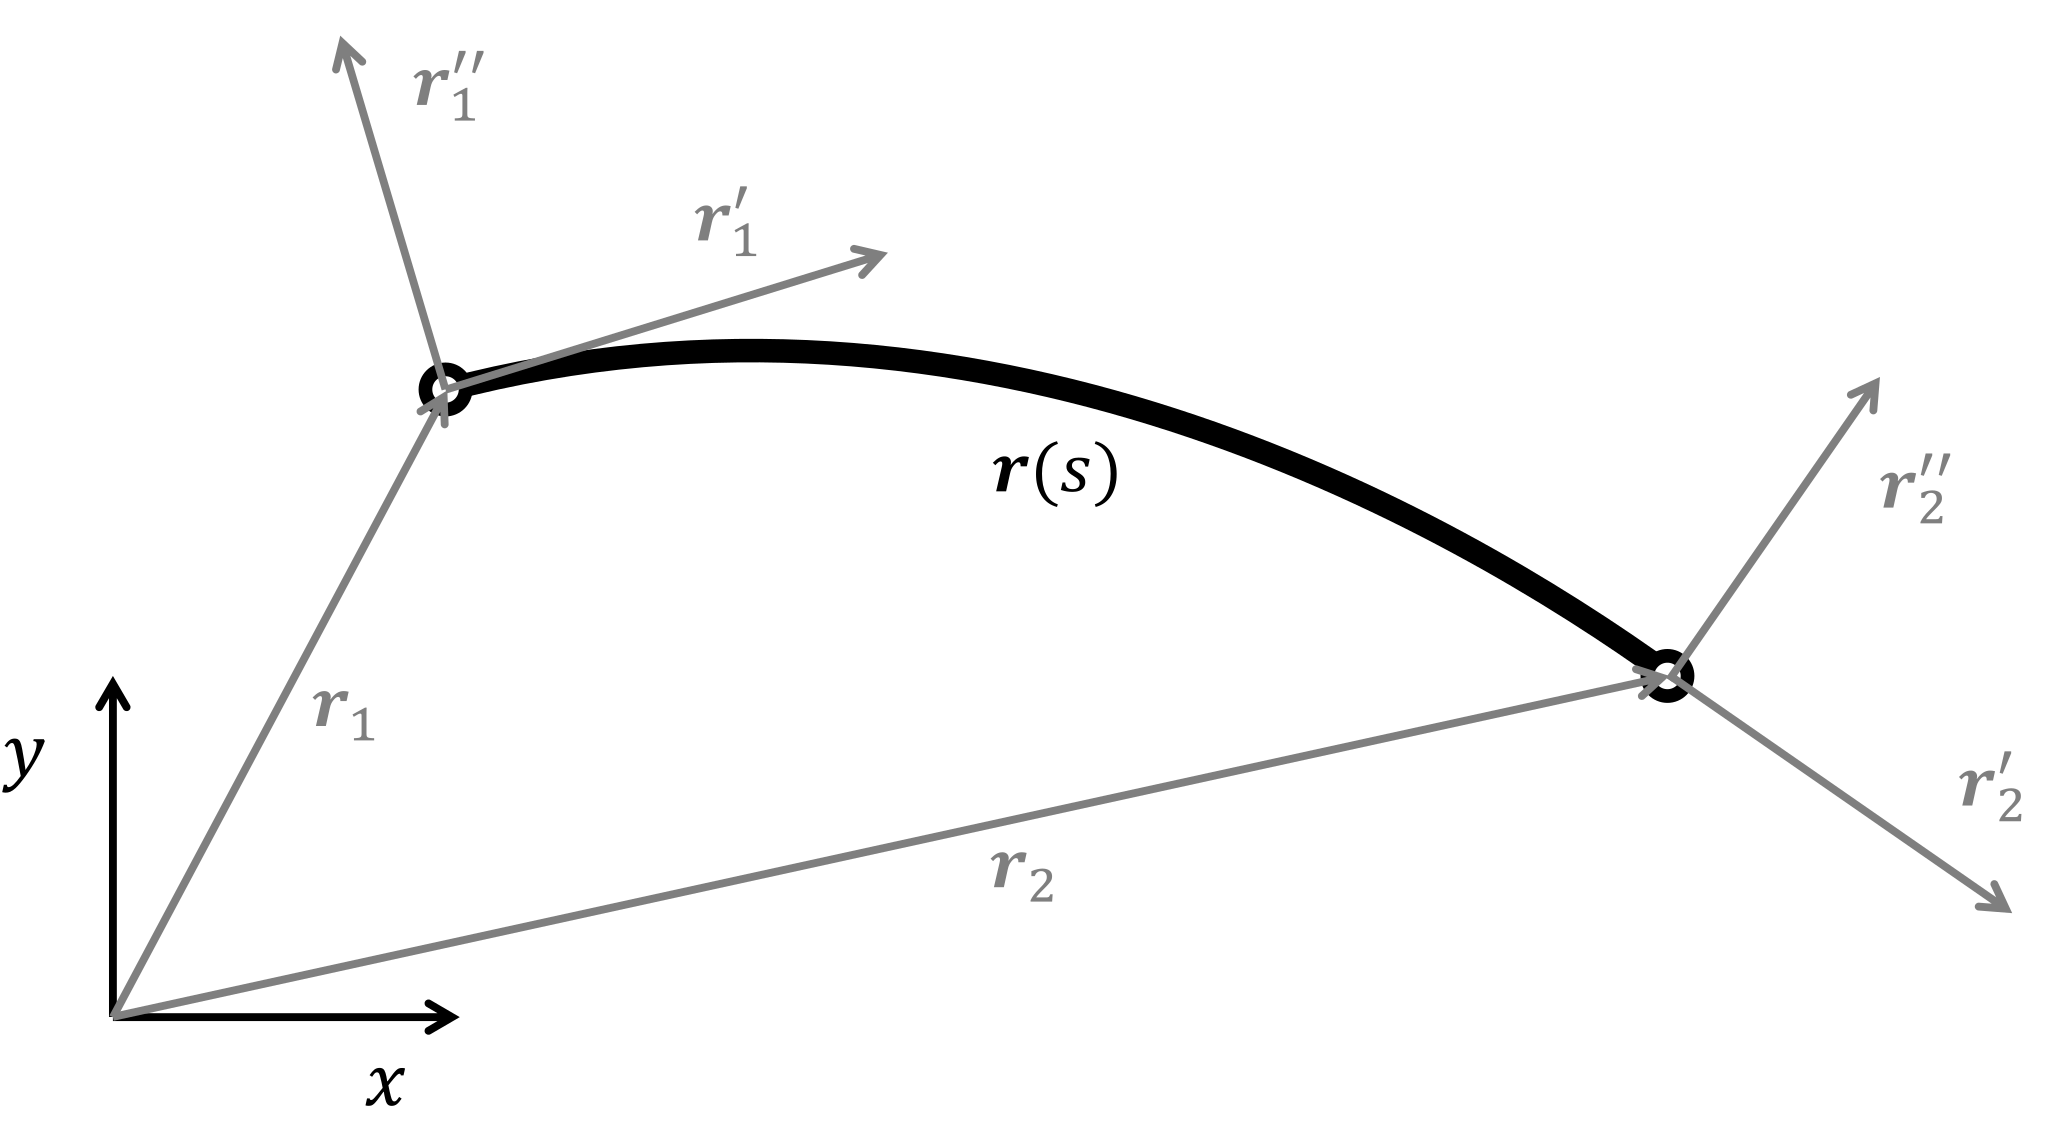
\includegraphics[width=0.7\textwidth]{figures/elements/beam-kinematics-shapefunctions}
\caption{Nodal coordinates of the beam element}
\label{fig:beam-kinematics-shapefunction}
\end{figure}

Figure \ref{fig:beam-kinematics-shapefunction} shows the nodal coordinates for our beam element, consisting of the position vectors $\boldsymbol{r}_{1,2}$ of the nodes as well as their gradients $\boldsymbol{r}'_{1,2}$ and $\boldsymbol{r}''_{1,2}$.
The continuous position $\boldsymbol{r}(s)$ of the beam axis is interpolated between the nodes by polynomial shape functions.

Most planar ANCF Euler-Bernoulli beam elements described in literature [source] use only the positions $\boldsymbol{r}$ and slopes $\boldsymbol{r}'$ of each node as the coordinates and interpolate the beam axis inbetween by cubic polynomials.
By choice of the nodal coordinates, these elements exhibit $C^1$ continuity, i.e. the slopes between adjacent elements are continuous.
However, since the curvature of the beam axis is proportional to $\boldsymbol{r}''$, the cubic interpolation does not enforce continuity of curvature and therefore strains and stresses can have jumps between elements.

That's why we also include the second derivatives of the beam axis as nodal coordinates and use higher order polynomials for interpolation.
This type of interpolation is also described in [source], where the authors call it the \textit{curvature constrained interpolation method}.
It results in an element with a total of 12 nodal coordinates, which makes it more expensive to compute than the standard ANCF beam element, but also more precise due to the higher order of interpolation, reducing the number of elements required to solve the same problem.

Before we continue, let's redefine the vector $\boldsymbol{r}$ as having only two dimensions in $x$ and $y$ direction for efficiency of implementation,

\begin{equation}
\boldsymbol{r}(s,\,t) = \begin{bmatrix}
r_x(s,\,t) \\
r_y(s,\,t)
\end{bmatrix} \in \mathbb{R}^2.\label{eq:beam-axis-2d}
\end{equation}

as opposed to the three-dimensional representation \ref{eq:beam-axis-3d} that we used for the general derivation.
According to figure \ref{fig:beam-kinematics-shapefunction}, the coordinate vector $\boldsymbol{u}(t) \in \mathbb{R}^{12}$ is defined as

\begin{equation}
\boldsymbol{u}(t) = \begin{bmatrix}
\boldsymbol{r}_{1}, & \boldsymbol{r}_{1}', & \boldsymbol{r}_{1}'', & \boldsymbol{r}_{2}, & \boldsymbol{r}_{2}', & \boldsymbol{r}_{2}''
\end{bmatrix}^\intercal.
\end{equation}

The position $\boldsymbol{r}$ of the beam axis depends on the parameter $s \in [s_{1},\,s_{2}]$ along the curve as well as the time $t$.
It is approximated by the product

\begin{equation}
\boldsymbol{r}(s, t) = \boldsymbol{S}(s)\,\boldsymbol{u}(t) \label{eq:ancf-position}
\end{equation}

of the coordinate vector with the matrix~$\boldsymbol{S}(s)$ of shape functions.
Similarly the first and second derivatives with respect to the parameter $s$ can be expressed in terms of the derivative of the shape functions as
%
\begin{align}
\boldsymbol{r}'(s, t) &= \boldsymbol{S}'(s)\,\boldsymbol{u}(t), \\
\boldsymbol{r}''(s, t) &= \boldsymbol{S}''(s)\,\boldsymbol{u}(t).
\end{align}

Using the length $l = s_{2} - s_{1}$ of the element in reference configuration, the natural coordinate $\zeta = (s - s_{1})/l$, and the quintic Hermite polynomials $S_1 \ldots S_6$, the shape functions are defined as [source]

% Last polynomial in the paper [ccim] seems to be wrong (3/2 -> 1/2)
% https://www.rose-hulman.edu/~finn/CCLI/Notes/day09.pdf
% https://github.com/tk-yoshimura/HermiteSpline

\begin{equation}
\boldsymbol{S}(s) =
\begin{bmatrix}
S_1\,\boldsymbol{I} & \vert & l\,S_2\,\boldsymbol{I} & \vert & l^2\,S_3\,\boldsymbol{I} & \vert & S_4\,\boldsymbol{I} & \vert & l\,S_5\,\boldsymbol{I} & \vert & l^2\,S_6\,\boldsymbol{I}
\end{bmatrix}
\end{equation}
%
\begin{align}
S_1 &= 1 - 10\,\zeta^3 + 15\,\zeta^4 - 6\,\zeta^5, & S_2 &= \zeta - 6\,\zeta^3 + 8\,\zeta^4 - 3\,\zeta^5, \notag \\
S_3 &= \frac{1}{2}\,\zeta^2 - \frac{3}{2}\,\zeta^3 + \frac{3}{2}\,\zeta^4 - \frac{1}{2}\zeta^5, & S_4 &= 10\,\zeta^3 - 15\,\zeta^4 + 6\,\zeta^5, \notag \\
S_5 &= -4\,\zeta^3 + 7\,\zeta^4 - 3\,\zeta^5 & S_6, &= \frac{1}{2}\,\zeta^3 - \zeta^4 + \frac{1}{2}\zeta^5.
\end{align}

With the first and second derivative being

\begin{equation}
\boldsymbol{S}'(s) =
\begin{bmatrix}
\frac{1}{l}\,S_1\,\boldsymbol{I} & \vert & S_2\,\boldsymbol{I} & \vert & l\,S_3\,\boldsymbol{I} & \vert & \frac{1}{l}\,S_4\,\boldsymbol{I} & \vert & S_5\,\boldsymbol{I} & \vert & l\,S_6\,\boldsymbol{I}
\end{bmatrix}
\end{equation}
%
\begin{align}
S_1' &= -30\,\zeta^2 + 60\,\zeta^3 - 30\,\zeta^4 & S_2' &= 1 - 18\,\zeta^2 + 32\,\zeta^3 - 15\,\zeta^4 \notag \\
S_3' &= \zeta - \frac{9}{2}\,\zeta^2 + 6\,\zeta^3 - \frac{5}{2}\zeta^4 & S_4' &= 30\,\zeta^2 - 60\,\zeta^3 + 30\,\zeta^4 \notag \\
S_5' &= -12\,\zeta^2 + 28\,\zeta^3 - 15\,\zeta^4 & S_6' &= \frac{3}{2}\,\zeta^2 - 4\,\zeta^3 + \frac{5}{2}\zeta^4
\end{align}

\begin{equation}
\boldsymbol{S}''(s) =
\begin{bmatrix}
\frac{1}{l^2}\,S_1\,\boldsymbol{I} & \vert & \frac{1}{l}\,S_2\,\boldsymbol{I} & \vert & S_3\,\boldsymbol{I} & \vert & \frac{1}{l^2}\,S_4\,\boldsymbol{I} & \vert & \frac{1}{l}\,S_5\,\boldsymbol{I} & \vert & S_6\,\boldsymbol{I}
\end{bmatrix}
\end{equation}
%
\begin{align}
S_1'' &= -60\,\zeta + 180\,\zeta^2 - 120\,\zeta^3 & S_2'' &= -36\,\zeta + 96\,\zeta^2 - 60\,\zeta^3 \notag \\
S_3'' &= 1 - 9\,\zeta + 18\,\zeta^2 - 10\,\zeta^3 & S_4'' &= 60\,\zeta - 180\,\zeta^2 + 120\,\zeta^3 \notag \\
S_5'' &= -24\,\zeta + 84\,\zeta^2 - 60\,\zeta^3 & S_6'' &= 3\,\zeta - 12\,\zeta^2 + 10\,\zeta^3
\end{align}

Those shape functions were stated here without any derivation, but it can be easily verified that they fulfill the nodal boundary conditions as illustrated in figure~\ref{fig:beam-kinematics-shapefunction}, which are
%
\begin{align}
\boldsymbol{r}(s_1, t) &= \boldsymbol{r}_{1}, & \boldsymbol{r}'(s_1, t) &= \boldsymbol{r}'_{1}, & \boldsymbol{r}''(s_1, t) &= \boldsymbol{r}''_{1}, \notag \\
\boldsymbol{r}(s_2, t) &= \boldsymbol{r}_{2}, & \boldsymbol{r}'(s_2, t) &= \boldsymbol{r}'_{2}, & \boldsymbol{r}''(s_2, t) &= \boldsymbol{r}''_{2}.
\end{align}

We use the interpolation (\ref{eq:ancf-position}) for the undeformed as well as the deformed states of the beam,
%
\begin{align}
\boldsymbol{r}_{t} &= \boldsymbol{r}(s,\,t) = \boldsymbol{S}(s)\,\boldsymbol{u}(t)\\
\boldsymbol{r}_{0} &= \boldsymbol{r}(s,\,0) = \boldsymbol{S}(s)\,\boldsymbol{u}(0)
\end{align}

which means that the undeformed state is described by the initial values $\boldsymbol{u}_0 = \boldsymbol{u}(0)$ of the nodal coordinates.
With this discretized kinematic description of the beam element in terms of nodal coordinates and shape functions we can now start developing the equation of motion of the element.

\subsection{Equation of motion}

According to the principal of virtual work [source], the virtual work $\delta W_{M}$ of the inertia forces and the virtual work of the internal forces $\delta W_{I}$ must be equal to the virtual work $\delta W_{E}$ of the external forces.

% http://shortcourse2018.it.cas.cz/im/data/my/2018_Lecture_08.pdf

\begin{equation}
\underbrace{\int_{V} \delta\boldsymbol{p}^\intercal\rho\,\ddot{\boldsymbol{p}}\,dV}_{\delta W_{M}} + \underbrace{\int_{V} \delta\boldsymbol{\varepsilon}^\intercal\boldsymbol{\sigma}\,dV}_{\delta W_{I}} = \underbrace{\delta\boldsymbol{u}^\intercal\boldsymbol{P}(t)}_{\delta W_{E}}
\end{equation}

%\begin{align}
%&\delta W_{M} + \delta W_{I} = \delta W_{E} \\
%\notag \\
%&\int_{V} \delta\boldsymbol{p}^\intercal\rho\,\ddot{\boldsymbol{p}}\,dV + \int_{V} \delta\boldsymbol{\varepsilon}^\intercal\boldsymbol{\sigma}\,dV = \delta\boldsymbol{u}^\intercal\boldsymbol{P}(t) \\
%\notag \\
%&\int_{V} \rho\left(\frac{\partial\boldsymbol{p}}{\partial\boldsymbol{u}}\delta\boldsymbol{u}\right)^\intercal\left(\frac{\partial\boldsymbol{p}}{\partial\boldsymbol{u}}\ddot{\boldsymbol{u}}\right)\,dV + \int_{V} \delta\varepsilon_{xx}\sigma_{xx}\,dV = \delta\boldsymbol{u}^\intercal\boldsymbol{P}(t) \\
%\notag \\
%&\delta\boldsymbol{u}^\intercal\underbrace{\left(\int_{V} \rho\,\frac{\partial\boldsymbol{p}}{\partial\boldsymbol{u}}^\intercal\frac{\partial\boldsymbol{p}}{\partial\boldsymbol{u}}\,dV\right)}_{\boldsymbol{M}}\ddot{\boldsymbol{u}} + \delta\boldsymbol{u}^\intercal \underbrace{\left(\int_{V} E\varepsilon_{xx}\,\frac{\partial \varepsilon_{xx}}{\partial \boldsymbol{u}}\,dV\right)}_{\boldsymbol{Q}(\boldsymbol{u})} = \delta\boldsymbol{u}^\intercal\boldsymbol{P}(t)
%\end{align}

\subsubsection{Mass matrix}

First we're going to look at the inertia forces and identify the element's mass matrix,
%
\begin{align}
\delta W_{M} &= \int_{V} \delta\boldsymbol{p}^\intercal\rho\,\ddot{\boldsymbol{p}}\,dV = \int_{V} \rho\left(\frac{\partial\boldsymbol{p}}{\partial\boldsymbol{u}}\delta\boldsymbol{u}\right)^\intercal\left(\frac{\partial\boldsymbol{p}}{\partial\boldsymbol{u}}\ddot{\boldsymbol{u}}\right)\,dV = \delta\boldsymbol{u}^\intercal\underbrace{\left(\int_{V} \rho\,\frac{\partial\boldsymbol{p}}{\partial\boldsymbol{u}}^\intercal\frac{\partial\boldsymbol{p}}{\partial\boldsymbol{u}}\,dV\right)}_{\boldsymbol{M}}\ddot{\boldsymbol{u}}.
\end{align}

Further expansion and simplification of the mass matrix leads to
%
\begin{align}
\boldsymbol{M} &= \int_{V} \rho\,\frac{\partial\boldsymbol{p}}{\partial\boldsymbol{u}}^\intercal\frac{\partial\boldsymbol{p}}{\partial\boldsymbol{u}}\,dV \notag \\
&= \int_{V} \rho\,\left(\frac{\partial\boldsymbol{r}}{\partial\boldsymbol{u}} + y\,\frac{\partial\boldsymbol{n}}{\partial\boldsymbol{u}}\right)^\intercal\left(\frac{\partial\boldsymbol{r}}{\partial\boldsymbol{u}} + y\,\frac{\partial\boldsymbol{n}}{\partial\boldsymbol{u}}\right)\,dV \notag \\
&= \int_{V} \left(\rho\,\frac{\partial\boldsymbol{r}}{\partial\boldsymbol{u}}^\intercal\frac{\partial\boldsymbol{r}}{\partial\boldsymbol{u}} + \rho y\,\frac{\partial\boldsymbol{n}}{\partial\boldsymbol{u}}^\intercal\frac{\partial\boldsymbol{r}}{\partial\boldsymbol{u}} + \rho y\,\frac{\partial\boldsymbol{r}}{\partial\boldsymbol{u}}^\intercal\frac{\partial\boldsymbol{n}}{\partial\boldsymbol{u}} + \rho y^2\,\frac{\partial\boldsymbol{n}}{\partial\boldsymbol{u}}^\intercal\frac{\partial\boldsymbol{n}}{\partial\boldsymbol{u}}\right)\,dV \notag \\
&= \int_{s_1}^{s_2} \left(\rho A\,\frac{\partial\boldsymbol{r}}{\partial\boldsymbol{u}}^\intercal\frac{\partial\boldsymbol{r}}{\partial\boldsymbol{u}} + \rho S\,\left(\frac{\partial\boldsymbol{n}}{\partial\boldsymbol{u}}^\intercal\frac{\partial\boldsymbol{r}}{\partial\boldsymbol{u}} + \frac{\partial\boldsymbol{r}}{\partial\boldsymbol{u}}^\intercal\frac{\partial\boldsymbol{n}}{\partial\boldsymbol{u}}\right) + \rho I\,\frac{\partial\boldsymbol{n}}{\partial\boldsymbol{u}}^\intercal\frac{\partial\boldsymbol{n}}{\partial\boldsymbol{u}}\right)\,ds
\end{align}

In the last step, the following three integrals over the beam's cross section have been factored out:
%
\begin{align}
\rho A(s) &= \int_A \rho\,dA \\
\rho S(s) &= \int_A \rho y\,dA \\
\rho I(s) &= \int_A \rho y^2\,dA
\end{align}

The first one, $\rho A$, is the linear density of the beam axis, i.e. the mass per unit length.
Mass matrix terms associated with this factor account for the overall motion of the beam axis.
The second term, $\rho S$, is the static moment of the cross section, weighted by its density, and is related to the excentricity of its center of gravity.
If the beam axis passed through the center of gravity of the cross sections, as is often assumed, this term would be zero.
Since we deliberately did not make this assumption, we will keep those terms.
The final term, $\rho I$ is the second moment of inertia of the section, weighted by its density, and accounts for the rotational inertia of the section itself.
It is usually neglected in Euler-Bernoulli theory because it is insignificantly small compared to the inertia of the beam axis.
However, since the absolute nodal coordinate formulation leads to a constant mass matrix that has to be computed only once, we will just keep this term because it barely adds any computational overhead.

The only thing left to do now is to express the derivatives $\nicefrac{\partial\boldsymbol{r}}{\partial\boldsymbol{u}}$ and $\nicefrac{\partial\boldsymbol{n}}{\partial\boldsymbol{u}}$ in terms of the shape function matrix $\boldsymbol{S}$.
This is straightforward for the first one and leads to

\begin{equation}
\frac{\partial\boldsymbol{r}}{\partial\boldsymbol{u}} = \frac{\partial}{\partial\boldsymbol{u}}\left(\boldsymbol{S}\boldsymbol{u}\right) = \boldsymbol{S}.
\end{equation}

For the second expression $\nicefrac{\partial\boldsymbol{n}}{\partial\boldsymbol{u}}$ however, we neglect the influence of longitudinal deformation and assume $|\boldsymbol{r}'| \approx |\boldsymbol{r}_{0}'|$ in order to preserve a constant mass matrix,

\begin{equation}
\frac{\partial\boldsymbol{n}}{\partial\boldsymbol{u}} = \frac{\partial}{\partial\boldsymbol{u}}\left(\boldsymbol{e}_{z} \times \frac{\boldsymbol{r}'}{|\boldsymbol{r}'|} \right) = \frac{\partial}{\partial\boldsymbol{u}}\left(\frac{\boldsymbol{T}\boldsymbol{S}'\boldsymbol{u}}{|\boldsymbol{r}'|} \right) \approx \frac{\boldsymbol{T}\boldsymbol{S}'}{|\boldsymbol{r}_{0}'|}.
\end{equation}

Putting everything together, the final mass matrix then becomes

\begin{equation}
\boldsymbol{M} = \int_{s_1}^{s_2} \left(\rho A\,\boldsymbol{S}^\intercal\boldsymbol{S} + \frac{\rho S}{|\boldsymbol{r}_{0}'|}\left(\boldsymbol{S}'^\intercal\boldsymbol{T}\boldsymbol{S} + \boldsymbol{S}\boldsymbol{T}\boldsymbol{S}'\right) + \frac{\rho I}{|\boldsymbol{r}_{0}'|^2}\boldsymbol{S}'^\intercal\boldsymbol{S}'\right)\,ds.
\end{equation}

It is indeed constant as promised, i.e. it doesn't depend on the nodal coordinates $\boldsymbol{u}$ and therefore has to be computed only once for each element.

\subsubsection{Internal forces}

The virtual work of the internal forces (ref) is expressed in terms of the strain vector $\boldsymbol{\varepsilon} \in \mathbb{R}^6$ that contains the strain components for all combinations of spatial directions and the vector $\boldsymbol{\sigma} \in \mathbb{R}^6$ that contains the corresponding stresses.
Our beam only has one non-zero strain component $\varepsilon_{xx}$ and for its associated stress we chose the linear-elastic material law $\sigma_{xx} = E\,\varepsilon_{xx}$ where $E$ is the elastic modulus or Young's modulus of the beam's material at the given position.

\begin{align}
\delta W_{I} &= \int_{V} \delta\boldsymbol{\varepsilon}^\intercal\boldsymbol{\sigma}\,dV = \int_{V} \delta\varepsilon_{xx}\sigma_{xx}\,dV = \int_{V} E\varepsilon_{xx}\delta\varepsilon_{xx}\,dV \notag \\
&= \delta\boldsymbol{u}^\intercal \underbrace{\int_{V} E\varepsilon_{xx}\frac{\partial\varepsilon_{xx}}{\partial\boldsymbol{u}}\,dV}_{\boldsymbol{Q}(\boldsymbol{u})}
\end{align}

With $\varepsilon_{xx} = \varepsilon - y\kappa$ according to equation (ref), the elastic forces expand to

\begin{align}
\boldsymbol{Q}(\boldsymbol{u}) &= \int_{V} E\left(\varepsilon - y\kappa\right)\left(\frac{\partial\varepsilon}{\partial\boldsymbol{u}} - y\frac{\partial\kappa}{\partial\boldsymbol{u}}\right)\,dV \notag \\
&= \int_{V}\left(E\,\varepsilon\frac{\partial\varepsilon}{\partial\boldsymbol{u}} - Ey\,\varepsilon\frac{\partial\kappa}{\partial\boldsymbol{u}} - Ey\,\kappa\frac{\partial\varepsilon}{\partial\boldsymbol{u}} + Ey^2\,\kappa\frac{\partial\kappa}{\partial\boldsymbol{u}}\right)\,dV \notag \\
&= \int_{s_1}^{s_2}\left(C_{\varepsilon\varepsilon}\,\varepsilon\frac{\partial\varepsilon}{\partial\boldsymbol{u}} + C_{\varepsilon\kappa}\,\varepsilon\frac{\partial\kappa}{\partial\boldsymbol{u}} + C_{\varepsilon\kappa}\,\kappa\frac{\partial\varepsilon}{\partial\boldsymbol{u}} + C_{\kappa\kappa}\,\kappa\frac{\partial\kappa}{\partial\boldsymbol{u}}\right)\,ds \notag \\
&= \int_{s_1}^{s_2}\left(\left(C_{\varepsilon\varepsilon}\,\varepsilon + C_{\varepsilon\kappa}\,\kappa\right)\frac{\partial\varepsilon}{\partial\boldsymbol{u}} + \left(C_{\kappa\kappa}\,\kappa + C_{\varepsilon\kappa}\,\varepsilon\right)\frac{\partial\kappa}{\partial\boldsymbol{u}}\right)\,ds
\end{align}

Again, the integral over the volumen of the element was reduced to one over its length by extracting integrals over the cross section area that can be assumed as known.
This time, they are
%
\begin{align}
C_{\varepsilon\varepsilon} &= \int_{A} E\,dA \\
C_{\varepsilon\kappa} &= \int_{A} Ey\,dA \\
C_{\kappa\kappa} &= \int_{A} Ey^2\,dA
\end{align}

They each represent a stiffness property of the cross section.
$C_{\varepsilon\varepsilon}$ is the stiffness against longitudinal deformation, $C_{\kappa\kappa}$ is the stiffness against bending deformation and $C_{\varepsilon\kappa}$ is the coupling stiffness between both deformation modes.
This coupling is present because the beam axis was not required to pass through the cross section's centroids.
We will later evaluate these integrals for the type of cross section that we're interested in.

The potential elastic energy of the element can be derived in a very similar way,
%
\begin{align}
\Pi &= \int_{V} \boldsymbol{\varepsilon}^\intercal\boldsymbol{\sigma}\,dV = \int_{V} E\,\varepsilon_{xx}^2\,dV = \int_{V} \left(E\,\varepsilon_{xx}^2 - 2Ey\,\varepsilon\kappa + Ey^2\,\kappa^2\right)\,dV \notag \\
&= \int_{s_1}^{s_2} \left(C_{\varepsilon\varepsilon}\,\varepsilon_{xx}^2 + 2C_{\varepsilon\kappa}\,\varepsilon\kappa + C_{\kappa\kappa}\,\kappa^2\right)\,ds
\end{align}

and uses the same cross section constants.
It can be verified that $\frac{\partial}{\partial\boldsymbol{u}}\Pi = \boldsymbol{Q}$, which shows that the elastic energy is a potential of the elastic forces.

The required derivatives of $\varepsilon$ and $\kappa$ with respect to the nodal coorsinates $\boldsymbol{u}$ are

\begin{align}
&\frac{\partial\varepsilon}{\partial\boldsymbol{u}} = \frac{\partial}{\partial\boldsymbol{r}'}\left(\frac{|\boldsymbol{r}'|}{|\boldsymbol{r}_{0}'|} - 1\right)\frac{\partial\boldsymbol{r}'}{\partial\boldsymbol{u}} = \frac{\boldsymbol{S}'^\intercal\boldsymbol{r}'}{|\boldsymbol{r}_{0}'||\boldsymbol{r}'|} \\
\notag \\
&\frac{\partial\kappa}{\partial\boldsymbol{u}} = \frac{\partial}{\partial\boldsymbol{u}}\left(\frac{|\boldsymbol{r}_{0}'|\kappa_{t} - |\boldsymbol{r}_{t}'|\kappa_{0}}{|\boldsymbol{r}_{0}'|^2}\right) = \frac{1}{|\boldsymbol{r}_{0}'|}\left(\frac{\partial\kappa_{t}}{\partial\boldsymbol{u}} - \kappa_0\,\frac{\partial\varepsilon}{\partial\boldsymbol{u}}\right) \\
\notag \\
&\frac{\partial}{\partial \boldsymbol{u}} \left(\boldsymbol{e}_{z}\left(\boldsymbol{r}' \times \boldsymbol{r}''\right)\right) = \frac{\partial}{\partial \boldsymbol{u}} \left(\boldsymbol{r}'^\intercal\boldsymbol{T}\boldsymbol{r}''\right) = \boldsymbol{S}'^\intercal\boldsymbol{T}\boldsymbol{r}'' - \boldsymbol{S}''^\intercal\boldsymbol{T}\boldsymbol{r}' \\
&\frac{\partial}{\partial \boldsymbol{u}} \left( |\boldsymbol{r}'|^2 \right) = 2\,|\boldsymbol{r}'| \frac{\partial |\boldsymbol{r}'|}{\partial \boldsymbol{u}} = 2\,|\boldsymbol{r}'| \frac{\boldsymbol{S}'^\intercal \boldsymbol{r}'}{|\boldsymbol{r}'|} = 2\,\boldsymbol{S}'^\intercal \boldsymbol{r}' \\
\notag \\
&\frac{\partial\kappa_{t}}{\partial \boldsymbol{u}} = \frac{|\boldsymbol{r}'|^2 \left( \boldsymbol{S}'^\intercal\boldsymbol{T}\boldsymbol{r}'' - \boldsymbol{S}''^\intercal\boldsymbol{T}\boldsymbol{r}' \right) - 2\left(\boldsymbol{e}_z\left( \boldsymbol{r}' \times \boldsymbol{r}'' \right)\right) \boldsymbol{S}'^\intercal\boldsymbol{r}' }{|\boldsymbol{r}'|^4} \notag \\
&\quad\quad = \frac{1}{|\boldsymbol{r}'|^2} \left( \boldsymbol{S}'^\intercal\boldsymbol{T}\boldsymbol{r}'' - \boldsymbol{S}''^\intercal\boldsymbol{T}\boldsymbol{r}' - 2\kappa_{T}\,\boldsymbol{S}'^\intercal\boldsymbol{r}' \right)
\end{align}




\subsubsection{Tangent stiffness matrix}

Obtaining the tangent stiffness matrix involves a whole lot of differentiation again, but is otherwise not particularly noteworthy.
The result is

\begin{multline}
\boldsymbol{K} = \frac{\partial \boldsymbol{Q}}{\partial \boldsymbol{u}} = \int_{s_1}^{s_2} \left( \left( C_{\varepsilon\varepsilon}\,\varepsilon + C_{\varepsilon\kappa}\,\kappa \right) \frac{\partial^2 \varepsilon}{\partial \boldsymbol{u}^2} + \left( C_{\kappa\kappa}\,\kappa + C_{\varepsilon\kappa}\,\varepsilon \right) \frac{\partial^2 \kappa}{\partial \boldsymbol{u}^2} + \ldots \right. \\ \left. C_{\varepsilon\varepsilon}\frac{\partial \varepsilon}{\partial \boldsymbol{u}}\frac{\partial \varepsilon}{\partial \boldsymbol{u}}^\intercal + C_{\varepsilon\kappa}\frac{\partial \varepsilon}{\partial \boldsymbol{u}}\frac{\partial \kappa}{\partial \boldsymbol{u}}^\intercal + C_{\varepsilon\kappa}\frac{\partial \kappa}{\partial \boldsymbol{u}}\frac{\partial \varepsilon}{\partial \boldsymbol{u}}^\intercal + C_{\kappa\kappa}\frac{\partial \kappa}{\partial \boldsymbol{u}}\frac{\partial \kappa}{\partial \boldsymbol{u}}^\intercal \right)\,ds
\end{multline}

with the intermediate derivatives

\begin{align}
&\frac{\partial^2\varepsilon}{\partial\boldsymbol{u}^2} = \frac{\boldsymbol{S}'^\intercal}{|\boldsymbol{r}_{0}'|}\frac{\partial}{\partial\boldsymbol{r}'}\left(\frac{\boldsymbol{r}'}{|\boldsymbol{r}'|}\right)\frac{\partial\boldsymbol{r}'}{\partial\boldsymbol{u}} = \frac{1}{|\boldsymbol{r}_{0}'||\boldsymbol{r}'|}\boldsymbol{S}'^\intercal\left(\boldsymbol{I} - \frac{\boldsymbol{r}'\boldsymbol{r}'^\intercal}{|\boldsymbol{r}'|^2}\right)\boldsymbol{S}' \\
\notag \\
&\frac{\partial^2\kappa}{\partial\boldsymbol{u}^2} = \frac{1}{|\boldsymbol{r}_{0}'|}\left(\frac{\partial^2\kappa_{t}}{\partial\boldsymbol{u}^2} - \kappa_0\,\frac{\partial^2\varepsilon}{\partial\boldsymbol{u}^2}\right) \\
\notag \\
&\frac{\partial^2 \kappa_{t}}{\partial \boldsymbol{u}^2} = \frac{\partial}{\partial \boldsymbol{u}}\left(\frac{\boldsymbol{f}}{g}\right) = \frac{g\frac{\partial \boldsymbol{f}}{\partial \boldsymbol{u}} - \boldsymbol{f}\frac{\partial g}{\partial \boldsymbol{u}}^\intercal}{g^2} = \frac{1}{|\boldsymbol{r}'|^2}\left(\frac{\partial\boldsymbol{f}}{\partial\boldsymbol{u}} - \frac{\partial\kappa_{t}}{\partial\boldsymbol{u}}\frac{\partial g}{\partial\boldsymbol{u}}^\intercal\right) \\
\notag \\
&\boldsymbol{f} = \boldsymbol{S}'^\intercal\boldsymbol{T}\boldsymbol{r}'' - \boldsymbol{S}''^\intercal\boldsymbol{T}\boldsymbol{r}' - 2\kappa_{T}\,\boldsymbol{S}'^\intercal\boldsymbol{r}' \\
&\frac{\partial \boldsymbol{f}}{\partial \boldsymbol{u}} = \boldsymbol{S}'^\intercal\boldsymbol{T}\boldsymbol{S}'' - \boldsymbol{S}''^\intercal\boldsymbol{T}\boldsymbol{S}' - 2\kappa_{T}\,\boldsymbol{S}'^\intercal\boldsymbol{S}' - 2\,\boldsymbol{S}'^\intercal\boldsymbol{r}'\frac{\partial \kappa_t}{\partial \boldsymbol{u}}^\intercal \\
\notag \\
&g = |\boldsymbol{r}'|^2 \\
&\frac{\partial g}{\partial \boldsymbol{u}} = 2\,\boldsymbol{S}'^\intercal\boldsymbol{r}'
\end{align}

\newpage

TODO: Explain where $V$ and $dV$ comes from

TODO: Explain energetic conjugate of the Biot stress, cite gerstmayr in that it is not necessary when only linear small strain material law is used

TODO: Explain where cross product matrix $\boldsymbol{T}$ comes from.

TODO: Replace $s$ with $x$.

TODO: Explain that integrals over the length of the element are done via Gauss(-Lobatto) integration.

\newpage
\subsection{Cross section properties}

Normal force:

\begin{align}
N(s) &= \int_A \sigma_{xx}\,dA = \int_A E\varepsilon_{xx}\,dA = \int_A E(\varepsilon - \kappa y) \notag \\
&= \left(\int_A E\,dA\right)\,\varepsilon + \left(-\int_A Ey\,dA\right)\,\kappa \notag \\
\notag \\
&= C_{\varepsilon\varepsilon}\varepsilon + C_{\varepsilon\kappa}\kappa
\end{align}

Bending moment:

\begin{align}
M(s) &= -\int_A \sigma_{xx}y\,dA = -\int_A E(\varepsilon y - \kappa y^2)\,dA \notag \\
&= \left(\int_A Ey^2\,dA\right)\,\kappa + \left(-\int_A Ey\,dA\right)\,\varepsilon \notag \\
\notag \\
&= C_{\kappa\kappa}\kappa + C_{\varepsilon\kappa}\varepsilon
\end{align}

Shear force, with $s^*$ being the actual arc length in the deformed state, probably...

\begin{equation}
Q(s) = \frac{dM}{ds^*} = \frac{dM}{ds}\frac{ds}{ds^*}
\end{equation}




\newpage
\subsection{Boundary conditions}

Properly constraining ANCF beam nodes requires some additional considerations because of the use of slopes and higher derivatives as the nodal coordinates.
Given is a start- or endpoint $i$ of a beam element as shown in figure \ref{fig:beam-element-boundary} with the position vector~$\boldsymbol{r}_{i}(t)$, the slope~$\boldsymbol{r}_{i}'(t)$ tangential to the beam and the second derivative~$\boldsymbol{r}_{i}''(t)$.

\begin{figure}[h]
\centering
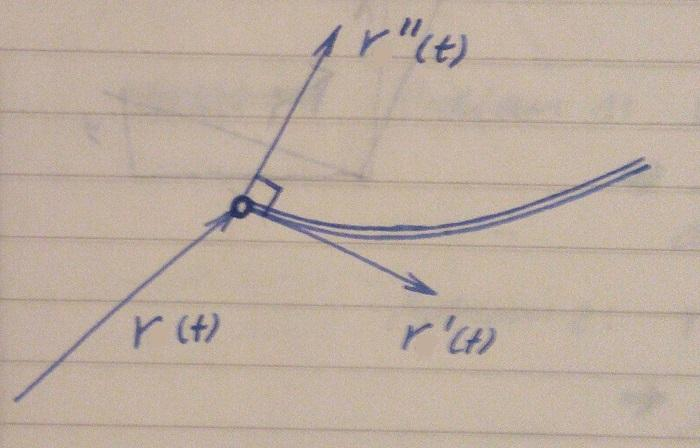
\includegraphics[width=0.5\textwidth]{figures/elements/beam-element-boundary}
\caption{Boundary conditions for an ANCF beam node (TODO: Add index $i$, also no right angle here!)}
\label{fig:beam-element-boundary}
\end{figure}

The initial values of those vectors at $t = 0$ are known as~$\boldsymbol{r}_{i}(0),\,\boldsymbol{r}_{i}'(0),\,\boldsymbol{r}_{i}''(0)$.

\textbf{Position}

Fixing the position of the node is straightforward, it just means that the position vector must always remain equal to its initial value,

\begin{equation}
\boldsymbol{r}_{i}(t) = \boldsymbol{r}_{i}(0).
\end{equation}

Those are effectively two constraints, one for each position coordinate.

\textbf{Rotation}

For fixing the rotation of the node, maybe because the beam is clamped at that point, it is tempting to constrain it by fixing its slope as
%
\begin{align}
\boldsymbol{r}'_{i}(t) &= \boldsymbol{r}'_{i}(0).
\end{align}

But this would actually overconstrain the node, since $\boldsymbol{r}_{i}'(t)$ not only encodes information about the direction of the beam axis but also about the elongation $\epsilon$, which we don't want to fix.
For similar reasons, the second derivative $\boldsymbol{r}''_{i}$ must remain unconstrained in order to not fix the curvature $\kappa$.

The correct way is to constrain the direction of $\boldsymbol{r}_{i}'(t)$, but not its magnitude $|\boldsymbol{r}_{i}'(t)|$.
Accordingly, the slope vector must be collinear with the initial slope, which can be expressed as the cross product

\begin{equation}
\boldsymbol{r}'(t) \times \boldsymbol{r}'(0) = 0, \label{eq:ancf-constraint-1}
\end{equation}

Equation (\ref{eq:ancf-constraint-1}) is only one scalar condition, so there remains one degree of freedom for the magnitude of the slope.
We know the initial tangent vector as

\begin{equation}
\boldsymbol{t}(0) = \frac{\boldsymbol{r}'(0)}{\lVert\boldsymbol{r}'(0)\rVert}
\end{equation}

and pick the magnitude of the slope as our degree of freedom,

\begin{equation}
u(t) = |\boldsymbol{r}_{i}'(t)|.
\end{equation}

Finally we write the slope vector as a product of $u(t)$ and the initial tangent vector,

\begin{equation}
\boldsymbol{r}_{i}'(t) = u_{1}(t)\cdot\boldsymbol{t}(0)
\end{equation}

Regarding the implementation, this amounts to a linear relationship between displacements as described in [TODO:cross-link].

\newpage
\subsection{Cross Sections (Old)}

The following derivations have been adapted from~\cite{bib:tm2} and~\cite{bib:wiki-sandwich}. Consider the laminated cross section shown in figure~\ref{fig:composite-sections-1}.
It is symmetric with respect to the~$y$-axis, bends/rotates around the~$z$-axis and consists of a number of rectangular layers. Each layer has its own density~$\rho_i$ and elastic modulus~$E_i$.
The geometry of the layers is given by their width~$w_i$, height~$h_i$ and center position~$y_i$.

\begin{figure}[h]
\centering
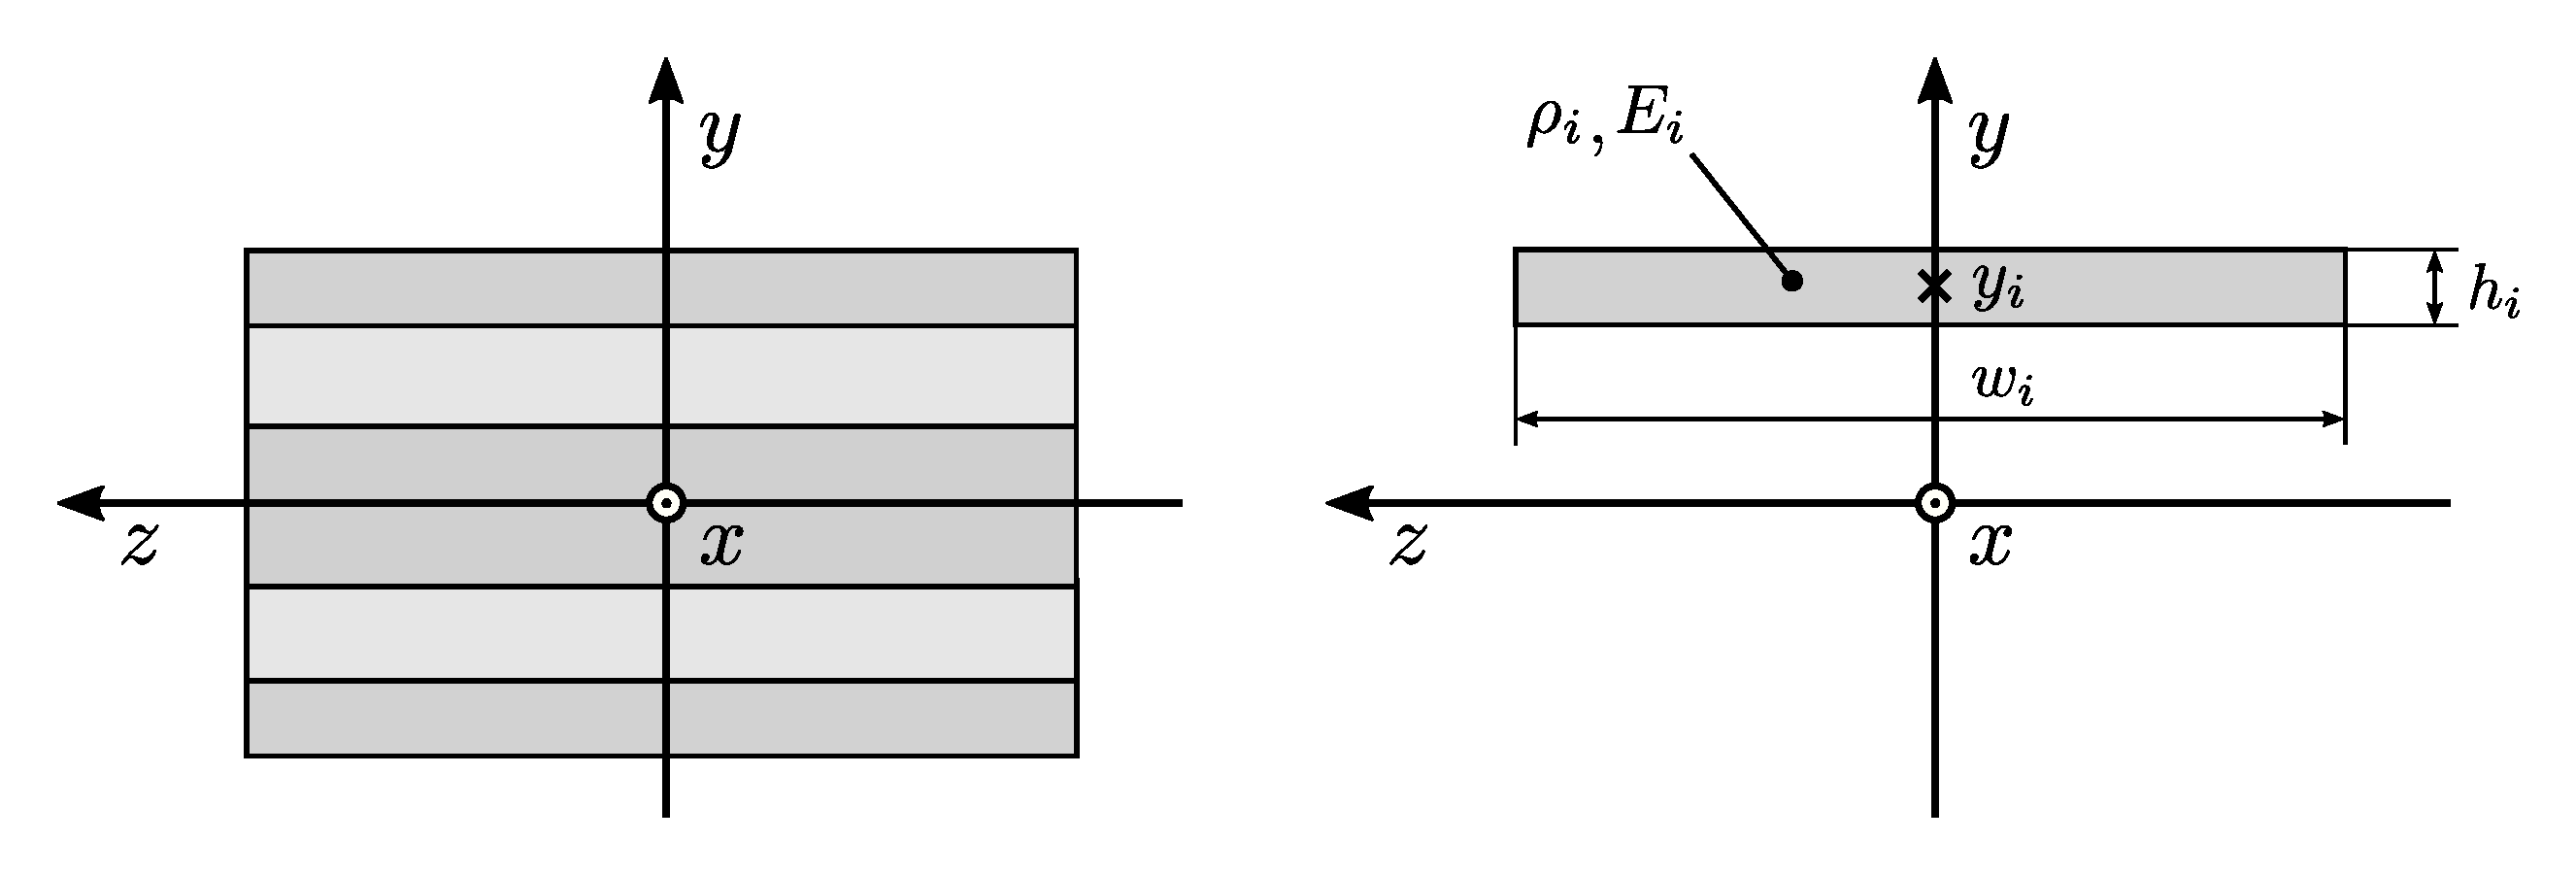
\includegraphics[width=0.9\textwidth]{figures/elements/composite-sections-1}
\caption{Composite cross section and single layer}
\label{fig:composite-sections-1}
\end{figure}

In Euler-Bernoulli beam theory the cross sections are assumed to stay flat and perpendicular to the beam axis during deformation.
We assume this to be true for our laminated cross section as well.
The distribution of longitudinal strain over the section is therefore given by the continuous function

\begin{equation}
\overline{\varepsilon}(y) = \varepsilon - \kappa\,y,
\end{equation}

where~$\varepsilon$ is the strain of the beam's centerline in $x$-direction and $\kappa$ its curvature around the $z$-axis.
The stress distribution however is not necessarily continuous, because each layer can have a different elastic modulus.
The stress within a layer is given by hooke's law as

\begin{equation}
\sigma_i(y) = E_i\cdot\overline{\varepsilon}(y),\quad y \in [y_i - \frac{h_i}{2},\,y_i + \frac{h_i}{2}].\label{eq:beam-stress-distribution}
\end{equation}

In order to determine the elastic constants in the constitutive equation~(\ref{eq:beam-constitutive}) we calculate the normal force~$N$ and bending moment~$M$ acting on the cross section by integrating the stresses~(\ref{eq:beam-stress-distribution}) over the section's area,

\begin{align}
N &= \int_A \sigma\,\mathrm{d}A = \sum_i\int_{A_i}\sigma_i\,\mathrm{d}A_i,\notag\\
&= \sum_i\int_{A_i}E_i\,\overline{\varepsilon}(y)\,\mathrm{d}A_i = \sum_i E_i \int_{A_i}(\varepsilon - \kappa\,y)\,\mathrm{d}A_i,\notag\\
&= \left(\sum_i E_i\int_{A_i}\mathrm{d}A_i\right)\varepsilon - \left(\sum_i E_i\int_{A_i}y\,\mathrm{d}A_i\right)\kappa,\notag\\
&=
\underbrace{
\left(\sum_i E_i\,A_i\right)
}_{C_{\varepsilon\varepsilon}}
\varepsilon
\underbrace{
- \left(\sum_i E_i\,A_i\,y_i\right)
}_{C_{\varepsilon\kappa}}
\kappa.\label{eq:elements:beam:constitutive_1}
\end{align}

The same can be done for the bending moment,

\begin{align}
M &= -\int_A y\,\sigma\,\mathrm{d}A = -\sum_i\int_{A_i}y\,\sigma_i\,\mathrm{d}A_i,\notag\\
&= -\sum_i\int_{A_i}y\,E_i\,(\varepsilon - \kappa\,y)\,\mathrm{d}A = -\sum_i\int_{A_i}(E_i\,\varepsilon\,y - E_i\,\kappa\,y^2)\,\mathrm{d}A,\notag\\
&= -\left(\sum_i E_i\int_{A_i}y\,dA_{i}\right)\varepsilon + \left(\sum_i E_i\int_{A_i}y^2\,dA_i\right)\kappa,\notag\\
&=
\underbrace{
-\left(\sum_i E_i\,A_i\,y_i\right)
}_{C_{\varepsilon\kappa}}
\varepsilon +
\underbrace{
\left(\sum_i E_i\,I_{i}\right)
}_{C_{\kappa\kappa}}
\kappa.\label{eq:elements:beam:constitutive_2}
\end{align}

The elastic constants describing the relationship between forces and deformation for the laminated cross section are therefore

\begin{align}
C_{\varepsilon\varepsilon} = \sum_i E_i\,A_i,\quad
C_{\kappa\kappa} = \sum_i E_i\,I_{i},\quad
C_{\varepsilon\kappa} = -\sum_i E_i\,A_i\,y_i.
\end{align}

In the case of the rectangular layers shown above, area~$A_i$ and second moment of inertia~$I_i$ evaluate to

\begin{align}
A_i &= w_i\,h_i,\\
I_i &= A_i\left(\frac{h_i^2}{12} + y_i^2\right).
\end{align}

Later we're also going to need the linear density (mass per unit length) of the laminated beam. It can be calculated by summing the the densities of the individual layers,

\begin{equation}
\overline{\rho A} = \sum_i \rho_i\,A_i.\label{eq:beam-linear-density}
\end{equation}

Pretty straightforward, compared to the other terms.
Overall, the stiffness relatio of the cross section is therefore

\begin{equation}
\begin{bmatrix}
N(s) \\ M(s)
\end{bmatrix}
=
\begin{bmatrix}
C_{ee}(s) & C_{ek}(s) \\
C_{ek}(s) & C_{kk}(s)
\end{bmatrix}
\cdot
\begin{bmatrix}
\varepsilon(s) \\ \kappa(s)
\end{bmatrix}
\end{equation}

Even though there is no shear deformation in Euler-Bernoulli beam theory, the total shear force~$Q(s)$ on the section can still be computed from static considerations as the first derivative~$M'(s)$ of the bending moment,

\begin{equation}
Q(s) = C_{kk}'(s)\,\kappa(s) + C_{ek}'(s)\,\varepsilon(s) + C_{kk}(s)\,\kappa'(s) + C_{ek}(s)\,\varepsilon'(s)
\end{equation}


\newpage
\section{String Element}

The string is modeled as an infinitely thin line with linear density $\rho A$, elasticity $EA$ and initial length $L$.

\begin{figure}[h]
\centering
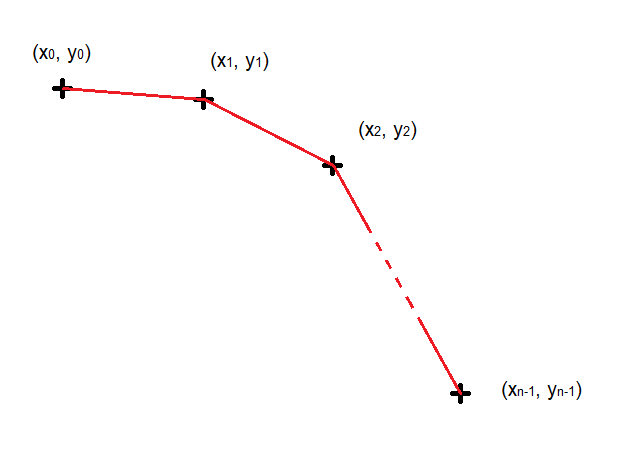
\includegraphics[width=0.6\linewidth]{figures/elements/string-element.png}
\caption{Model of the string}
\label{fig:elements:string-element}
\end{figure}

\subsection{Single string element}

Displacement vector $\boldsymbol{u} = (x_0,\,y_0,\,x_1,\,y_1)^\intercal$. The current length of the element is

$$
\overline{L}(\boldsymbol{u}) = \sqrt{(x_{1} - x{0})^2 + (y_{1} - y{0})^2}.
$$

Each point on the element can be described by the line

\begin{align*}
r(s,\,\boldsymbol{u}) &= \begin{bmatrix} x_0 \\ y_0 \end{bmatrix}(1 - \zeta) + \begin{bmatrix} x_1 \\ y_1 \end{bmatrix} \zeta, \quad \zeta = \frac{s}{L} \in [0,\,1] \\
&=
\begin{bmatrix}
1 - \zeta & 0 & \zeta & 0 \\
0 & 1 - \zeta & 0 & \zeta
\end{bmatrix}
\begin{bmatrix}
x_0 \\ y_0 \\ x_1 \\ y_1
\end{bmatrix}
\\
&= \boldsymbol{S}(s) \cdot \boldsymbol{u}
\end{align*}

Kinetic energy of the element

\begin{align*}
T &= \frac{1}{2}\,\rho A \, \int_{0}^{L} \dot{r}(s)^\intercal\,\dot{r}(s)\,ds \\
&= \frac{1}{2}\,\dot{\boldsymbol{u}}^\intercal \underbrace{\left( \rho A \int_0^L \boldsymbol{S}^\intercal(s) \boldsymbol{S}(s)\,ds \right)}_{\boldsymbol{M}}\,\dot{\boldsymbol{u}} \\
\boldsymbol{M} &= \rho AL
\begin{bmatrix}
\nicefrac{1}{3} & 0 & \nicefrac{1}{6} & 0 \\
0 & \nicefrac{1}{3} & 0 & \nicefrac{1}{6} \\
\nicefrac{1}{6} & 0 & \nicefrac{1}{3} & 0 \\
0 & \nicefrac{1}{6} & 0 & \nicefrac{1}{3}
\end{bmatrix}
\end{align*}

\subsection{String with one contact point}

Displacement vector $\boldsymbol{u} = (x_0,\,y_0,\,x_1,\,y_1,\,x_2,\,y_2)^\intercal$. The current length of the element is

$$
\overline{L}(\boldsymbol{u}) =
\underbrace{
\sqrt{(x_{1} - x{0})^2 + (y_{1} - y{0})^2}
}_{\overline{L}_{01}}
+
\underbrace{
\sqrt{(x_{2} - x{1})^2 + (y_{2} - y{1})^2}
}_{\overline{L}_{12}}
$$

Assuming constant strain over the length of the string, the initial arc length $s$ and elongated arc length $\overline{s}$ have a constant ratio,

\begin{align*}
\frac{s}{\overline{s}} = \frac{L}{\overline{L}}
\end{align*}

$$
r(s,\,\boldsymbol{u}) =
\begin{cases} 
 r_0(s,\,\boldsymbol{u}), & \text{if } s \in [ 0, \, \frac{\overline{L}_1}{\overline{L}}L [ \\
 r_1(s,\,\boldsymbol{u}), & \text{if } s \in [ \frac{\overline{L}_1}{\overline{L}}L, \, L ]
\end{cases}
$$

\begin{align*}
r_{01}(\zeta,\,\boldsymbol{u}) &= \begin{bmatrix} x_0 \\ y_0 \end{bmatrix}(1 - \zeta) + \begin{bmatrix} x_1 \\ y_1 \end{bmatrix} \zeta
=
\underbrace{
\begin{bmatrix}
1 - \zeta & 0 & \zeta & 0 & 0 & 0\\
0 & 1 - \zeta & 0 & \zeta & 0 & 0
\end{bmatrix}
}_{\boldsymbol{S}_{01}(\zeta)}
\boldsymbol{u} \\
r_{12}(\zeta,\,\boldsymbol{u}) &= \begin{bmatrix} x_1 \\ y_1 \end{bmatrix}(1 - \zeta) + \begin{bmatrix} x_2 \\ y_2 \end{bmatrix} \zeta
=
\underbrace{
\begin{bmatrix}
0 & 0 & 1 - \zeta & 0 & \zeta & 0 \\
0 & 0 & 0 & 1 - \zeta & 0 & \zeta
\end{bmatrix}
}_{\boldsymbol{S}_{12}(\zeta)}
\boldsymbol{u}
\end{align*}

\begin{align*}
T &= \frac{1}{2}\rho A  \left( \int_{0}^{L_{01}} \dot{r}_{01}^\intercal(\zeta(s), \boldsymbol{u})\,\dot{r}_{01}(\zeta(s), \boldsymbol{u})\,ds + \int_{0}^{L_{12}} \dot{r}^\intercal_{12}(\zeta(s), \boldsymbol{u})\,\dot{r}_{12}(\zeta(s), \boldsymbol{u})\,ds \right)
\end{align*}

Transformation with $\zeta(s) = \frac{s}{L_{ij}}$ and $\zeta'(s) = \frac{1}{L_{ij}}$:

\begin{align*}
T &= \frac{1}{2}\rho A  \left( L_{01} \int_{0}^{1} \dot{r}_{01}^\intercal(\zeta, \boldsymbol{u})\,\dot{r}_{01}(\zeta, \boldsymbol{u})\,d\zeta + L_{12} \int_{0}^{1} \dot{r}^\intercal_{12}(\zeta, \boldsymbol{u})\,\dot{r}_{12}(\zeta, \boldsymbol{u})\,d\zeta \right) \\
&= \frac{1}{2} \dot{\boldsymbol{u}}^\intercal \rho A \left( L_{01} \int_{0}^{1} \boldsymbol{S}_{01}^\intercal(\zeta)\,\boldsymbol{S}_{01}(\zeta)\,d\zeta +  L_{12} \int_{0}^{1} \boldsymbol{S}^\intercal_{12}(\zeta)\,\boldsymbol{S}_{12}(\zeta)\,d\zeta \right) \dot{\boldsymbol{u}} \\
&= \frac{1}{2} \dot{\boldsymbol{u}}^\intercal \rho A L \left( \frac{\overline{L}_{01}}{\overline{L}} \int_{0}^{1} \boldsymbol{S}_{01}^\intercal(\zeta)\,\boldsymbol{S}_{01}(\zeta)\,d\zeta + \frac{\overline{L}_{12}}{\overline{L}} \int_{0}^{1} \boldsymbol{S}^\intercal_{12}(\zeta)\,\boldsymbol{S}_{12}(\zeta)\,d\zeta \right) \dot{\boldsymbol{u}}
\end{align*}

\newpage

The elongated length $\overline{L}$ can be calculated as the sum of the distances between the points,

$$
\overline{L} = \sum_{i=0}^{n-2} L_{i}
$$

with the distances $\overline{L}_{i}$ between point $p_{i}$ and $p_{i+1}$ being

$$
\overline{L}_{i} = \sqrt{(x_{i+1} - x{i})^2 + (y_{i+1} - y{i})^2}.
$$

Each segment line can be described as the line

$$
r_{i}(t) = p_{i} + (p_{i+1} - p_{i}) \cdot t, \quad t \in [0,\,1].
$$

In order to parametrize this by arc length, we distinguish between the arc length $s$ along the undeformed string and the arc length $\overline{s}$ along the elongated string.
If we assume that the string is internally in static equilibrium at all times, the strain in the string is evenly distributed, i.e. constant and we can write

\begin{align*}
\frac{s}{\overline{s}} = \frac{L}{\overline{L}}
\end{align*}

Furthermore, within a single line segment, we have $\overline{s} = t \cdot \overline{L}_{i}$, so we can express $t$ as

\begin{align*}
t = \frac{s}{\overline{L}_{i}}\frac{\overline{L}}{L}
\end{align*}

The kinetic energy of the string is

\begin{align*}
T &= \frac{1}{2}\,\rho A \, \int_{0}^{L} \dot{r}(s)^\intercal\,\dot{r}(s)\,ds \\
&= \frac{1}{2}\,\rho A \, \sum_{i=0}^{n-2} \int_{t=0}^{t=1} \dot{r}_{i}(s)^\intercal\,\dot{r}_{i}(s)\,ds \\
&= \frac{1}{2}\,\rho A \, \sum_{i=0}^{n-2} \int_{0}^{\frac{\overline{L}_{i}\overline{L}}{L}} \dot{r}_{i}(s)^\intercal\,\dot{r}_{i}(s)\,ds \\
\end{align*}
